\documentclass[a4paper,11pt,twoside]{memoir}
\chapterstyle{veelo}

\renewcommand*{\printchaptertitle}[1]{%
    \hrule\vskip\onelineskip \raggedleft \chaptitlefont #1}


% TODO before completion: improve graphics by running dia-export.sh

% TODO check: always , before and

% TODO all \cite, \ref: always ~ instead of standard space to avoid line breaking

% TODO all captions: end sentence with a dot (.)

\usepackage{TUINFDA}

\definecolor{linkcolor}{HTML}{000088}

\usepackage{url}
\usepackage[colorlinks=true,linkcolor=linkcolor,urlcolor=linkcolor,citecolor=linkcolor]{hyperref}	% links in pdf
\usepackage{bookmark}
\usepackage{graphicx}            			% Figures
\usepackage{verbatim}            			% Code-Environment
\usepackage[lined,linesnumbered,algochapter]{algorithm2e} % Algorithm-Environment

\usepackage{pgf}					
\usepackage{tikz}					% tikz graphics

\usepackage{comment}
\usepackage{siunitx}
\sisetup{per-mode=symbol}

% TODO remove glossary number lists (with option nonumberlist)?
\usepackage[toc,xindy,numberedsection=autolabel]{glossaries}
\renewcommand{\glsnamefont}[1]{\makefirstuc{#1}} % for making the first word of each glossary term upper case
\renewcommand{\glsseeitemformat}[1]{\Glsentrytext{#1}}
\newcommand{\Egls}[1]{\emph{\Gls{#1}}}
\newcommand{\egls}[1]{\emph{\gls{#1}}}
\renewcommand{\glsseelastsep}{\space\emph{and}\space}

\makeglossary

\newglossaryentry{temperature}{
  name={temperature},
  description={Sub-concept of \emph{Weather phenomenon} representing temperature. Sub-concepts are \emph{Frost}, \emph{Cold}, \emph{Below room temperature}, \emph{Room temperature}, \emph{Above room temperature}, and \emph{Heat}},
  see={weather phenomenon,frost,cold,below room temperature,room temperature,above room temperature,heat}
}
\newglossaryentry{room temperature}{
  name={room temperature},
  description={Sub-concept of \emph{Temperature} representing a temperature of least 20 and at most 25 degrees Celsius},
  see={temperature}
}
\newglossaryentry{above room temperature}{
  name={abobe room temperature},
  description={Sub-concept of \emph{Temperature} representing a temperature of more than 25 and less than or equal to 30 degrees Celsius},
  see={temperature}
}
\newglossaryentry{below room temperature}{
  name={below room temperature},
  description={Sub-concept of \emph{Temperature} representing a temperature of more than or equal to 10 and less than 20 degrees Celsius},
  see={temperature}
}
\newglossaryentry{cold}{
  name={cold},
  description={Sub-concept of \emph{Temperature} representing a temperature  of more than or equal to 0 and less than 10 degrees Celsius},
  see={temperature}
}
\newglossaryentry{frost}{
  name={frost},
  description={Sub-concept of \emph{Temperature} representing a temperature  below 0 degrees Celsius},
  see={temperature}
}
\newglossaryentry{heat}{
  name={heat},
  description={Sub-concept of \emph{Temperature} representing a temperature  above 30 degrees Celsius},
  see={temperature}
}


% TODO sub-concepts of sun position: "sub-concept of..."
\newglossaryentry{sun position}{
  name={sun position},
  description={Sub-concept of \emph{Weather phenomenon} describing the position of the sun, given by its elevation above horizon and its direction. Sub-concepts are \emph{Day}, \emph{Solar twilight}, \emph{Twilight}, \emph{Civil twilight}, \emph{Nautical twilight}, \emph{Astronomical twilight}, and \emph{Night} for the elevation above horizon, and \emph{Sun from north}, \emph{Sun from east}, \emph{Sun from South}, and \emph{Sun from West} for the direction.},
  see={weather phenomenon,day,solar twilight,twilight,civil twilight,nautical twilight,astronomical twilight,night,sun from north,sun from east,sun from south,sun from west}
}
\newglossaryentry{day}{
  name={day},
  description={During the day, the sun is exactly at or above the horizon},
  see={sun position}
}
\newglossaryentry{night}{
  name={night},
  description={The sun is more than 18 degrees below horizon},
  see={sun position}
}
\newglossaryentry{solar twilight}{
  name={solar twilight},
  description={During solar twilight, the sun is above horizon, but less than 6 degrees above},
  see={sun position,day}
}
\newglossaryentry{sun below horizon}{
  name={sun below horizon},
  description={The sun is below the horizon},
  see={sun position,night,twilight}
}
\newglossaryentry{twilight}{
  name={twilight},
  description={During twilight, the sun is not at or above horizon and at most 18 degrees below horizon},
  see={sun position,civil twilight,nautical twilight,astronomical twilight}
}
\newglossaryentry{civil twilight}{
  name={civil twilight},
  description={During civil twilight, the sun is not at or above horizon and at most 6 degrees below horizon},
  see={sun position,twilight}
}
\newglossaryentry{nautical twilight}{
  name={nautical twilight},
  description={During nautical twilight, the sun is more than 6 degrees and no more than 12 degrees below horizon},
  see={sun position,twilight}
}
\newglossaryentry{astronomical twilight}{
  name={astronomical twilight},
  description={During astronomical twilight, the sun is more than 12 degrees and no more than 18 degrees below horizon},
  see={sun position,twilight}
}
\newglossaryentry{sun from north}{
  name={sun from north},
  description={The direction of the sun's position of more than 315 or at most 45 degrees},
  see={sun position}
}
\newglossaryentry{sun from east}{
  name={sun from east},
  description={The direction of the sun's position of more than 45 and at most 135 degrees},
  see={sun position}
}
\newglossaryentry{sun from south}{
  name={sun from south},
  description={The direction of the sun's position of more than 135 and at most 225 degrees},
  see={sun position}
}
\newglossaryentry{sun from west}{
  name={sun from west},
  description={The direction of the sun's position of more than 225 and at most 315 degrees},
  see={sun position}
}


\newglossaryentry{atmospheric pressure}{
  name={atmospheric pressure},
  description={Sub-concept of \emph{Weather phenomenon} representing atmospheric pressure. Sub-concepts are \emph{Very low pressure}, \emph{Low pressure}, \emph{Average pressure}, \emph{High pressure}, and \emph{Very high pressure}},
  see={weather phenomenon,very low pressure,low pressure,average pressure,high pressure,very high pressure}
}
\newglossaryentry{very low pressure}{
  name={very low pressure},
  description={Sub-concept of \emph{Atmospheric pressure} representing a pressure of less than \unit{998}\hecto\pascal},
  see={atmospheric pressure}
}
\newglossaryentry{low pressure}{
  name={low pressure},
  description={Sub-concept of \emph{Atmospheric pressure} representing a pressure of at least 998 and less than \unit{1008}\hecto\pascal},
  see={atmospheric pressure}
}
\newglossaryentry{average pressure}{
  name={average pressure},
  description={Sub-concept of \emph{Atmospheric pressure} representing a pressure of at least 1008 and less than \unit{1018}\hecto\pascal},
  see={atmospheric pressure}
}
\newglossaryentry{high pressure}{
  name={high pressure},
  description={Sub-concept of \emph{Atmospheric pressure} representing a pressure of at least 1018 and less than \unit{1028}\hecto\pascal},
  see={atmospheric pressure}
}
\newglossaryentry{very high pressure}{
  name={very high pressure},
  description={Sub-concept of \emph{Atmospheric pressure} representing a pressure of at least \unit{1028}\hecto\pascal},
  see={atmospheric pressure}
}


\newglossaryentry{wind}{
  name={wind},
  description={Sub-concept of \emph{Weather phenomenon} representing wind (speed and direction, the latter is optional). Sub-concepts are \emph{Directional wind}, \emph{North wind}, \emph{East wind}, \emph{South wind}, and \emph{West wind} for the wind direction, and \emph{Calm}, \emph{Light wind}, \emph{Strong wind}, \emph{Storm}, and \emph{Hurricane} for the wind speed},
  see={weather phenomenon,directional wind,north wind,east wind,south wind,west wind,calm,light wind,strong wind,storm,hurricane}
}
\newglossaryentry{directional wind}{
  name={directional wind},
  description={Sub-concept of \emph{Wind} including a direction},
  see={wind,north wind,east wind,south wind,west wind}
}
\newglossaryentry{north wind}{
  name={north wind},
  description={Sub-concept of \emph{Wind} representing wind approximately coming from the north, e.g. originating from a direction of at least 315 or less than 45 degrees},
  see={wind,directional wind}
}
\newglossaryentry{east wind}{
  name={east wind},
  description={Sub-concept of \emph{Wind} representing wind approximately coming from the east, e.g. originating from a direction of at least 45 and less than 135 degrees},
  see={wind,directional wind}
}
\newglossaryentry{south wind}{
  name={south wind},
  description={Sub-concept of \emph{Wind} representing wind approximately coming from the south, e.g. originating from a direction of at least 135 and less than 225 degrees},
  see={wind,directional wind}
}
\newglossaryentry{west wind}{
  name={wind wind},
  description={Sub-concept of \emph{Wind} representing wind  approximately coming from the wind, e.g. originating from a direction of at least 225 and less than 315 degrees},
  see={wind,directional wind}
}
\newglossaryentry{calm}{
  name={calm},
  description={Sub-concept of \emph{Wind} representing wind with a speed below \unit{1}\metre\per\second},
  see={wind}
}
\newglossaryentry{light wind}{
  name={light wind},
  description={Sub-concept of \emph{Wind} representing wind with a speed of at least 1 and less than \unit{10}\metre\per\second},
  see={wind}
}
\newglossaryentry{strong wind}{
  name={strong wind},
  description={Sub-concept of \emph{Wind} representing wind with a speed of at least 10 and less than \unit{20}\metre\per\second},
  see={wind}
}
\newglossaryentry{storm}{
  name={storm},
  description={Sub-concept of \emph{Wind} representing wind  with a speed of at least \unit{20}\metre\per\second},
  see={wind}
}
\newglossaryentry{hurricane}{
  name={hurricane},
  description={Sub-concept of \emph{Wind} representing wind with a speed of at least \unit{32}\metre\per\second},
  see={wind}
}


\newglossaryentry{cloud cover}{
  name={cloud cover},
  description={Sub-concept of \emph{Weather phenomenon} describing the current cloud coverage in \emph{okta} (integer numbers from 0 to 9). Sub-concepts are \emph{Clear sky}, \emph{Partly cloudy}, \emph{Mostly cloudy}, \emph{Overcast}, and \emph{Unknown cloud cover}},
  see={weather phenomenon,okta,clear sky,partly cloudy,mostly cloudy,overcast,unknown cloud cover}
}
\newglossaryentry{okta}{
  name={okta},
  description={Unit of measurement that specifies the amount of \emph{cloud cover} on a range from 0 (\emph{Clear sky}) to 8 (\emph{Overcast}); a value of 9 represents an \emph{Unknown cloud cover}},
  see={cloud cover,clear sky,partly cloudy,mostly cloudy,overcast,unknown cloud cover}
}
\newglossaryentry{clear sky}{
  name={clear sky},
  description={Sub-concept of \emph{Cloud cover} representing cloud coverage that is reported to be 0$\:$\emph{okta}},
  see={okta,cloud cover}
}
\newglossaryentry{partly cloudy}{
  name={partly cloudy},
  description={Sub-concept of \emph{Cloud cover} representing cloud coverage that is reported to be 1, 2, 3 or 4$\:$\emph{okta}},
  see={okta,cloud cover}
}
\newglossaryentry{mostly cloudy}{
  name={mostly cloudy},
  description={Sub-concept of \emph{Cloud cover} representing cloud coverage that is reported to be 5, 6, or 7$\:$\emph{okta}},
  see={okta,cloud cover}
}
\newglossaryentry{overcast}{
  name={overcast},
  description={Sub-concept of \emph{Cloud cover} representing cloud coverage that is reported to be 8$\:$\emph{okta}},
  see={okta,cloud cover}
}
\newglossaryentry{unknown cloud cover}{
  name={unknown cloud cover},
  description={Sub-concept of \emph{Cloud cover} representing cloud coverage that is reported to be 9$\:$\emph{okta}},
  see={okta,cloud cover}
}

\newglossaryentry{weather report}{
  name={weather report},
  description={Concept that summarizes all data aquired at a certain \emph{observation time} for a certain \emph{location} from a \emph{weather source}, about the current weather or the weather some time in the future. Exactly one \emph{weather state} is linked to each \emph{weather report}},
  see={weather state,current weather report,forecast weather report,weather source,observation time,start time,end time,location}
}
\newglossaryentry{current weather report}{
  name={current weather report},
  description={Sub-concept of \emph{Weather report} describing the current weather},
  see={weather report}
}
\newglossaryentry{weather report from sensor}{
  name={current weather report from sensor},
  description={Sub-concept of \emph{weather report}; contains data obtained from one or more \emph{sensor sources}},
  see={weather report,sensor source}
}
\newglossaryentry{weather report from service}{
  name={current weather report from service},
  description={Sub-concept of \emph{weather report}; contains data obtained from an Internet \emph{service source}},
  see={weather report,service source}
}
\newglossaryentry{current weather report from sensor}{
  name={current weather report from sensor},
  description={Sub-concept of \emph{Current weather report}; compiled from data from a \emph{sensor source}},
  see={weather report,current weather report,sensor source}
}
\newglossaryentry{current weather report from service}{
  name={current weather report from service},
  description={Sub-concept of \emph{Current weather report}; compiled from data from a \emph{service source}},
  see={weather report,current weather report,service source}
}
\newglossaryentry{forecast weather report}{
  name={forecast weather report},
  description={Sub-concept of \emph{Weather report} for some time after its \emph{observation time}},
  see={weather report,observation time,short range weather report,medium range weather report,long range weather report}
}
\newglossaryentry{short range weather report}{
  name={short range weather report},
  description={Sub-concept of \emph{Weather report} describing a forecast for a point of time at most 3 hours in the future relative to the \emph{observation time}},
  see={weather report,forecast weather report,observation time}
}
\newglossaryentry{medium range weather report}{
  name={medium range weather report},
  description={Sub-concept of \emph{Weather report} describing a forecast for a point of time more than 3 hours and less than 12 hours in the future relative to the \emph{observation time}},
  see={weather report,forecast weather report,observation time}
}
\newglossaryentry{long range weather report}{
  name={long range weather report},
  description={Sub-concept of \emph{Weather report} describing a forecast for a point of time at least 12 hours in the future relative to the \emph{observation time}},
  see={weather report,forecast weather report,observation time}
}
\newglossaryentry{observation time}{
  name={observation time},
  description={The time when the weather data was collected from the weather sensor or the Internet weather service, given by an instance of the concept \emph{Instant} from \emph{OWL-Time}\cite{owl-time}},
  see={weather report,has observation time}
}
\newglossaryentry{has observation time}{
  name={observation time},
  description={An object property of \emph{Weather report} that specifies the report's \emph{observation time}},
  see={weather report,observation time}
}
\newglossaryentry{start time}{
  name={start time},
  description={The time a \emph{Weather report} is valid from, given by an instance of the concept \emph{Interval} from \emph{OWL-Time}\cite{owl-time} that specifies the interval between the report's \emph{observation time} and its \emph{start time}},
  see={weather report,has start time,end time,observation time}
}
\newglossaryentry{end time}{
  name={end time},
  description={The time a \emph{Weather report} is valid until, given by an instance of the concept \emph{Interval} from \emph{OWL-Time}\cite{owl-time} that specifies the interval between the report's \emph{observation time} and its \emph{end time}},
  see={weather report,has end time,start time,observation time}
}
\newglossaryentry{has start time}{
  name={has start time},
  description={An object property of \emph{weather report} that specifies the report's \emph{start time}},
  see={weather report,start time, has end time,observation time}
}
\newglossaryentry{has end time}{
  name={has end time},
  description={An object property of \emph{weather report} that specifies the report's \emph{end time}},
  see={weather report,end time,has start time,observation time}
}
\newglossaryentry{priority}{
  name={priority},
  description={An integer value indicating which \emph{weather report} for a certain period of time is to be preferred over another \emph{weather report} for the same period of time},
  see={weather report,has priority}
}
\newglossaryentry{has priority}{
  name={has priority},
  description={A data property of \emph{weather report} that specifies the report's \emph{priority}},
  see={weather report,priority}
}


\newglossaryentry{dew point}{
  name={dew point},
  description={Sub-concept of \emph{Weather phenomenon} that describes the dew point},
  see={weather phenomenon}
}


\newglossaryentry{humidity}{
  name={humidity},
  description={Sub-concept of \emph{Weather phenomenon} representing the relative humidity of the air. Sub-concepts are \emph{Very dry}, \emph{Dry}, \emph{Normal humidity}, \emph{Moist}, and \emph{Very moist}},
  see={weather phenomenon,very dry,dry,normal humidity,moist,very moist}
}
\newglossaryentry{very dry}{
  name={very dry},
  description={Sub-concept of \emph{Humidity} describing relative humidity of less than 30 percent},
  see={humidity}
}
\newglossaryentry{dry}{
  name={dry},
  description={Sub-concept of \emph{Humidity} describing relative humidity of at least 30 and less than 40 percent},
  see={humidity}
}
\newglossaryentry{normal humidity}{
  name={normal humidity},
  description={Sub-concept of \emph{Humidity} describing relative humidity of at least 40 and at most 70 percent},
  see={humidity}
}
\newglossaryentry{moist}{
  name={moist},
  description={Sub-concept of \emph{Humidity} describing relative humidity of more than 70 and at most 80 percent},
  see={humidity}
}
\newglossaryentry{very moist}{
  name={very moist},
  description={Sub-concept of \emph{Humidity} describing relative humidity of more than 80 percent},
  see={humidity}
}



\newglossaryentry{precipitation}{
  name={precipitation},
  description={Sub-concept of \emph{Weather phenomenon} that describes precipitation (intensity and probability). Sub-concepts are \emph{No rain}, \emph{Light rain}, \emph{Medium rain}, \emph{Heavy rain}, \emph{Extremely heavy rain}, and \emph{Tropical storm rain}},
  see={weather phenomenon,no rain,light rain,medium rain,heavy rain,extremely heavy rain,tropical storm rain}
}
\newglossaryentry{no rain}{
  name={no rain},
  description={Sub-concept of \emph{Precipitation} representing absence precipitation (because either the intensity of precipitation is 0)},
  see={precipitation}
}
\newglossaryentry{light rain}{
  name={light rain},
  description={Sub-concept of \emph{Precipitation} representing a precipitation probability greater than 0 and an intensity of more than 0 and at most \unit{5}\milli\metre\per\hour},
  see={precipitation}
}
\newglossaryentry{medium rain}{
  name={medium rain},
  description={Sub-concept of \emph{Precipitation} representing a precipitation probability greater than 0 and an intensity of more than 5 and at most \unit{20}\milli\metre\per\hour},
  see={precipitation}
}
\newglossaryentry{heavy rain}{
  name={heavy rain},
  description={Sub-concept of \emph{Precipitation} representing a precipitation probability greater than 0 and an intensity of more than 20 and at most \unit{50}\milli\metre\per\hour},
  see={precipitation}
}
\newglossaryentry{extremely heavy rain}{
  name={extremely heavy rain},
  description={Sub-concept of \emph{Precipitation} representing a precipitation probability greater than 0 and an intensity of more than 50 and at most \unit{100}\milli\metre\per\hour},
  see={precipitation}
}
\newglossaryentry{tropical storm rain}{
  name={tropical storm rain},
  description={Sub-concept of \emph{Precipitation} representing a precipitation probability greater than 0 and an intensity of more than \unit{100}\milli\metre\per\hour},
  see={precipitation}
}


\newglossaryentry{solar radiation}{
  name={solar radiation},
  description={Sub-concept of \emph{Weather phenomenon} representing solar radiation. Sub-concepts are \emph{No radiation}, \emph{Low radiation}, \emph{Mediumr radiation}, \emph{High radiation}, and \emph{Very high radiation}},
  see={weather phenomenon,no radiation,low radiation,medium radiation,high radiation,very high radiation}
}
\newglossaryentry{no radiation}{
  name={no radiation},
  description={Sub-concept of \emph{Solar radiation} describing the absence of any solar radiation (\unit{0}\watt\per\squaren\metre)},
  see={solar radiation}
}
\newglossaryentry{low radiation}{
  name={low radiation},
  description={Sub-concept of \emph{Solar radiation} describing solar radiation of more than \unit{0}\watt\per\squaren\metre and less than \unit{250}\watt\per\squaren\metre},
  see={solar radiation}
}
\newglossaryentry{medium radiation}{
  name={medium radiation},
  description={Sub-concept of \emph{Solar radiation} describing solar radiation of at least \unit{250}\watt\per\squaren\metre and less than \unit{500}\watt\per\squaren\metre},
  see={solar radiation}
}
\newglossaryentry{high radiation}{
  name={high radiation},
  description={Sub-concept of \emph{Solar radiation} describing solar radiation of at least \unit{500}\watt\per\squaren\metre and less than \unit{750}\watt\per\squaren\metre},
  see={solar radiation}
}
\newglossaryentry{very high radiation}{
  name={very high radiation},
  description={Sub-concept of \emph{Solar radiation} describing solar radiation of at least \unit{750}\watt\per\squaren\metre},
  see={solar radiation}
}


\newglossaryentry{location}{
  name={location},
  description={An object property of \emph{weather report} that specifies the geographical position the \emph{weather report} is valid for, given by \emph{altitude}, \emph{longitude} and \emph{latitude}, using the \emph{WGS84} reference model\cite{WGS84}; links to an instance of the concept \emph{point} of the \emph{Basic Geo (WGS84 lat/long) Vocabulary}\cite{wgs84_vocabulary}},
  see={weather report,lat,long,alt}
}
\newglossaryentry{lat}{
  name={lat},
  description={Latitude of the \emph{location} a \emph{weather report} is valid for, given as a decimal number. Positive values refer to positions north of the equator, negative values refer to positions south of the equator}, % TODO mention: property from WGS84; reference WGS84
  see={weather report,location}
}
\newglossaryentry{long}{
  name={long},
  description={Longitude of the \emph{location} a \emph{weather report} is valid for, given as a decimal number. Positive values refer to positions east of the prime meridian at Greenwich, negative values refer to positions west of the prime meridian}, % TODO mention: property from WGS84; reference WGS84
  see={weather report,location}
}
\newglossaryentry{alt}{
  name={alt},
   description={Height above \emph{MSL} (\emph{mean sea level}) of the \emph{location} the \emph{weather report} is valid for, in metres}, % TODO mention: property from WGS84; reference WGS84
  see={weather report,location}
}


\newglossaryentry{weather source}{
  name={weather source},
  description={A concept representing a source for weather data, either a set of \emph{weather sensors} or an Internet \emph{weather service}. Sub-concepts are \emph{Sensor source}, and \emph{Service source}},
  see={sensor source,service source}
}
\newglossaryentry{sensor source}{
  name={sensor source},
  description={A sub-concept of \emph{Weather Source} representing a sensor or a set of sensors offering some kind of weather data},
  see={weather source}
}
\newglossaryentry{service source}{
  name={service source},
  description={A sub-concept of \emph{Weather Source} representing an Internet weather service offering some kind of weather data},
  see={weather source}
}

\newglossaryentry{weather condition}{
  name={weather condition},
  description={A concept describing the overall state of the weather, represented by (a combination of) these individuals: \emph{Sun}, \emph{Light clouds}, \emph{Partly cloudy}, \emph{Cloudy}, \emph{Fog}, \emph{Rain}, \emph{Snow}, \emph{Sleet}, and \emph{Thunder}},
  see={weather state}
}
\newglossaryentry{weather phenomenon}{
  name={weather phenomenon},
  description={A concept that represents a certain weather element. Relevant weather elements are \emph{Atmospheric pressure}, \emph{Cloud cover}, \emph{Dew point}, \emph{Humidity}, \emph{Precipitation}, \emph{Solar radiation}, \emph{Sun position}, \emph{Temperature}, and \emph{Wind}},
  see={atmospheric pressure,cloud cover,dew point,humidity,precipitation,solar radiation,sun position,temperature,wind}
}

\newglossaryentry{weather state}{
  name={weather state},
  description={A concept that represents all data available about weather phenomena for a certain \emph{Weather report}. A set of instances of the concept \emph{Weather phenomenon} are linked to every instance of \emph{Weather state}},
  see={weather report,weather phenomenon}
}


\newglossaryentry{has source}{
  name={has source},
  description={Object property that links instances of \emph{Weather report} and \emph{Weather source}; inverse property of \emph{is source of}},
  see={weather report,weather source,is source of}
}
\newglossaryentry{is source of}{
  name={is source of},
  description={Object property that links instances of \emph{Weather report} and \emph{Weather source}; inverse property of \emph{has source}},
  see={weather report,weather source,has source}
}
\newglossaryentry{has weather state}{
  name={has weather state},
  description={Object property that links instances of \emph{Weather report} and \emph{Weather state}; inverse property of \emph{belongs to weather report}},
  see={weather report,weather state,belongs to weather report}
}
\newglossaryentry{belongs to weather report}{
  name={belongs to weather report},
  description={Object property that links instances of \emph{Weather report} and \emph{Weather state}; inverse property of \emph{has weather state}},
  see={weather report,weather state,has weather state}
}
\newglossaryentry{has condition}{
  name={has condition},
  description={Object property that links instances of \emph{Weather state} and \emph{Weather condition}; does not have an inverse property},
  see={weather state,weather condition}
}
\newglossaryentry{has weather phenomenon}{
  name={has weather phenomenon},
  description={Object property that links instances of \emph{Weather state} and \emph{Weather phenomenon}; inverse property of \emph{belongs to state}},
  see={weather state,weather phenomenon,belongs to state}
}
\newglossaryentry{belongs to state}{
  name={belongs to state},
  description={Object property that links instances of \emph{Weather state} and \emph{Weather phenomenon}; inverse property of \emph{has weather phenomenon}},
  see={weather state,weather phenomenon,has weather phenomenon}
}

% TODO
\newglossaryentry{has cloud altitude}{
  name={has cloud altitude},
  description={TODO},
  see={}
}
\newglossaryentry{has cloud cover}{
  name={has cloud cover},
  description={TODO},
  see={}
}
\newglossaryentry{has dew point value}{
  name={has dew point value},
  description={TODO},
  see={}
}
\newglossaryentry{has humidity value}{
  name={has humidity value},
  description={TODO},
  see={}
}
\newglossaryentry{has precipitation probability}{
  name={has precipitation probability},
  description={TODO},
  see={}
}
\newglossaryentry{has precipitation intensity}{
  name={has precipitation intensity},
  description={TODO},
  see={}
}
\newglossaryentry{has pressure value}{
  name={has pressure value},
  description={TODO},
  see={}
}
\newglossaryentry{has solar radiation value}{
  name={has solar radiation value},
  description={TODO},
  see={}
}
\newglossaryentry{has sun direction}{
  name={has sun direction},
  description={TODO},
  see={}
}
\newglossaryentry{has sun elevation angle}{
  name={has sun elevation angle},
  description={TODO},
  see={}
}
\newglossaryentry{has temperature value}{
  name={has temperature value},
  description={TODO},
  see={}
}
\newglossaryentry{has wind direction}{
  name={has wind direction},
  description={TODO},
  see={}
}
\newglossaryentry{has wind speed}{
  name={has wind speed},
  description={TODO},
  see={}
}

\newglossaryentry{has previous weather state}{
  name={has previous weather state},
  description={TODO},
  see={}
}
\newglossaryentry{has next weather state}{
  name={has next weather state},
  description={TODO},
  see={}
}


\usepackage[english]{babel,varioref}	% Querverweise
\usepackage{bibgerm,cite}       % Deutsche Bezeichnungen, Automatisches Zusammenfassen von Literaturstellen
% to use the german charset include cp850 for MS-DOS, ansinew for Windows and latin1 for Linux.
% \usepackage[latin1]{inputenc}

\usepackage{mdframed}
\usepackage{longtable}
\usepackage{listings}
\usepackage{xspace}

\thesistitle{A Weather Ontology for Predictive Control in Smart Homes}
%\thesissubtitle{Optional Subtitle} % optional

% TODO
\thesisdate{TT.MM.2013}

% all titles and designations have to be gender-related!
\thesisdegree{Diplom-Ingenieur}{Diplom-Ingenieur}
\thesiscurriculum{Software Engineering \& Internet Computing}{Software Engineering \& Internet Computing} % your study
\thesisverfassung{Verfasser} % Verfasser
\thesisauthor{Paul Staroch} % your name
\thesisauthoraddress{Graf Starhemberg-Gasse 5, 1040 Wien} % your address
\thesismatrikelno{0425426} % your registration number

\thesisbetreins{Ao.Univ.Prof. Dipl.-Ing. Dr.techn. Wolfgang Kastner}
\thesisbetrzwei{Dipl.-Ing. Mario Kofler}

% define page numbering styles
\makepagestyle{numberCorner}
\makeevenhead{numberCorner}{\thepage}{}{\leftmark}
\makeoddhead{numberCorner}{\rightmark}{}{\thepage}
\makeevenfoot{numberCorner}{}{}{}
\makeoddfoot{numberCorner}{}{}{}

% define custom macros for specific formats or names
\newcommand{\uml}[1]{\texttt{#1}}
\newcommand{\cd}{\textsf{Class Diagram}}

\newcommand{\thinkhome}{\emph{ThinkHome}\xspace}
\newcommand{\smarthome}{\emph{Smart Home}\xspace}
\newcommand{\smarthomes}{\emph{Smart Homes}\xspace}
\newcommand{\thinkhomeweather}{\emph{ThinkHomeWeather}\xspace}
\newcommand{\methontology}{\emph{METHONTOLOGY}\xspace}
\newcommand{\protege}{\emph{Prot\'{e}g\'{e}}\xspace}
\newcommand{\yrno}{\emph{yr.no}\xspace}
\newcommand{\chapterquotation}[2]{\hfill\parbox{0.5\textwidth}{\raggedleft\noindent\textit{#1}\\--\enskip #2}}

\makeatletter
\newenvironment{btHighlight}[1][]
{\begingroup\tikzset{bt@Highlight@par/.style={#1}}\begin{lrbox}{\@tempboxa}}
{\end{lrbox}\bt@HL@box[bt@Highlight@par]{\@tempboxa}\endgroup}

\newcommand\btHL[1][]{%
  \begin{btHighlight}[#1]\bgroup\aftergroup\bt@HL@endenv%
}
\def\bt@HL@endenv{%
  \end{btHighlight}%   
  \egroup
}
\newcommand{\bt@HL@box}[2][]{%
  \tikz[#1]{%
    \pgfpathrectangle{\pgfpoint{1pt}{0pt}}{\pgfpoint{\wd #2}{\ht #2}}%
    \pgfusepath{use as bounding box}%
    \node[anchor=base west, fill=orange!30,outer sep=0pt,inner xsep=1pt, inner ysep=0pt, rounded corners=0pt, minimum height=\ht\strutbox+1pt,#1]{\raisebox{1pt}{\strut}\strut\usebox{#2}};
  }%
}
\makeatother

\setcounter{maxsecnumdepth}{2}

\begin{document}

\captionnamefont{\bfseries}

%%%%%%%%%%%%%%%%%%%%%%%%%%%%%%%%%%%%%%%%%
%%%   FRONTMATTER    %%%%%%%%%%%%%%%%%%%%
%%%%%%%%%%%%%%%%%%%%%%%%%%%%%%%%%%%%%%%%%
\frontmatter
\pagenumbering{roman}

%%%%%%%%%%%%%%%%%%%%%%%%%%%%%%%%%%%%%%%%%
%%%   TITLEPAGES    %%%%%%%%%%%%%%%%%%%%%
%%%%%%%%%%%%%%%%%%%%%%%%%%%%%%%%%%%%%%%%%

% the german title page is required as first page
% $Id: titlepage.tex 1752 2010-03-20 11:07:02Z tkren $
%
% TU Wien - Faculty of Informatics
% thesis titlepage
%
% This titlepage is using the geometry package, see
% <http://www.ctan.org/macros/latex/contrib/geometry/geometry.pdf>
%
% For questions and comments send an email to
% Thomas Krennwallner <tkren@kr.tuwien.ac.at>
% or to Petra Brosch <brosch@big.tuwien.ac.at>
%

\selectlanguage{ngerman}

% setup page dimensions for titlepage
\newgeometry{left=2.4cm,right=2.4cm,bottom=2.5cm,top=2cm}

% force baselineskip and parindent
\newlength{\tmpbaselineskip}
\setlength{\tmpbaselineskip}{\baselineskip}
\setlength{\baselineskip}{13.6pt}
\newlength{\tmpparindent}
\setlength{\tmpparindent}{\parindent}
\setlength{\parindent}{17pt}

% first titlepage
\thispagestyle{tuinftitlepage}

%
% Kludge: for each titlepage set \pagenumbering to a different
% style. This is used to fix a problem with hyperref, because there
% are multiple "page 1" and hyperref hates that
%
\pagenumbering{Alph}

\begin{center}
{\ \vspace{3.4cm}}

\begin{minipage}[t][2.8cm][s]{\textwidth}%
\centering
\thesistitlefontHUGE\sffamily\bfseries\tuinfthesistitle\\
\bigskip
{\thesistitlefonthuge\sffamily\bfseries\tuinfthesissubtitle}
\end{minipage}

\vspace{1.3cm}

{\thesistitlefontLARGE\sffamily \tuinfthesistype}

\vspace{6mm}

{\thesistitlefontlarge\sffamily zur Erlangung des akademischen Grades}

\vspace{6mm}

{\thesistitlefontLARGE\sffamily\bfseries \tuinfthesisdegree}

\vspace{6mm}

{\thesistitlefontlarge\sffamily im Rahmen des Studiums}

\vspace{6mm}

{\thesistitlefontLarge\sffamily\bfseries \tuinfthesiscurriculum}

\vspace{6.5mm}

{\thesistitlefontlarge\sffamily eingereicht von}

\vspace{6mm}

{\thesistitlefontLarge\sffamily\bfseries \tuinfthesisauthor}

\vspace{1.5mm}

{\thesistitlefontlarge\sffamily Matrikelnummer \tuinfthesismatrikelno} 

\vspace{1.4cm}

\vspace{0pt}\raggedright\thesistitlefontnormalsize\sffamily
\begin{minipage}[t][1.6cm][t]{\textwidth}%
  %
  an der

  Fakult\"{a}t f\"{u}r Informatik der Technischen Universit\"{a}t Wien
\end{minipage}

\begin{minipage}[t][4cm][t]{\textwidth}%
  \vspace{0pt}\raggedright\thesistitlefontnormalsize\sffamily
  %
  \begin{tabbing}%
	    \hspace{19mm} \= \hspace{66mm} \kill
	    \tuinfthesisbetreuung: \> \tuinfthesisbetreins\\
	    Mitwirkung: \> \tuinfthesisbetrzwei\\
	                \> \tuinfthesisbetrdrei
  \end{tabbing}
\end{minipage}

\begin{minipage}[t][1.5cm][t]{\textwidth}%
  \vspace{0pt}\sffamily\thesistitlefontnormalsize
  \begin{tabbing}%
    \hspace{45mm} \= \hspace{63mm} \= \hspace{51mm} \kill
    Wien, \tuinfthesisdate \> {\raggedright\rule{51mm}{0.5pt}} \> {\raggedright\rule{51mm}{0.5pt}} \\
    \> \begin{minipage}[t][0.5cm][t]{51mm}\centering (Unterschrift \tuinfthesisverfassung)\end{minipage}
    \> \begin{minipage}[t][0.5cm][t]{51mm}\centering (Unterschrift \tuinfthesisbetreuung)\end{minipage}
    \end{tabbing}
\end{minipage}

\end{center}

% we want an empty page right after first titlepage
\pagestyle{empty}
\cleardoublepage

% we're done with the titlepages, proceed with default pagenumbering
\pagenumbering{roman}

% restore baselineskip
\setlength{\baselineskip}{\tmpbaselineskip}
\setlength{\parindent}{\tmpparindent}

% back to normal geometry
\restoregeometry

\selectlanguage{english}

%%% Local Variables:
%%% TeX-PDF-mode: t
%%% TeX-debug-bad-boxes: t
%%% TeX-parse-self: t
%%% TeX-auto-save: t
%%% reftex-plug-into-AUCTeX: t
%%% End:


% an english translation may follow
% $Id: titlepage.tex 1752 2010-03-20 11:07:02Z tkren $
%
% TU Wien - Faculty of Informatics
% thesis titlepage
%
% This titlepage is using the geometry package, see
% <http://www.ctan.org/macros/latex/contrib/geometry/geometry.pdf>
%
% For questions and comments send an email to
% Thomas Krennwallner <tkren@kr.tuwien.ac.at>
% or to Petra Brosch <brosch@big.tuwien.ac.at>
%

% setup page dimensions for titlepage
\newgeometry{left=2.4cm,right=2.4cm,bottom=2.5cm,top=2cm}

% force baselineskip and parindent
%\newlength{\tmpbaselineskip}
%\setlength{\tmpbaselineskip}{\baselineskip}
%\setlength{\baselineskip}{13.6pt}
%\newlength{\tmpparindent}
%\setlength{\tmpparindent}{\parindent}
%\setlength{\parindent}{17pt}

% first titlepage
\thispagestyle{tuinftitlepage}

%
% Kludge: for each titlepage set \pagenumbering to a different
% style. This is used to fix a problem with hyperref, because there
% are multiple "page 1" and hyperref hates that
%
\pagenumbering{Roman}

\begin{center}
{\ \vspace{3.4cm}}

\begin{minipage}[t][2.8cm][s]{\textwidth}%
\centering
\thesistitlefontHUGE\sffamily\bfseries\tuinfthesistitle\\
\bigskip
{\thesistitlefonthuge\sffamily\bfseries\tuinfthesissubtitle}
\end{minipage}

\vspace{1.3cm}

{\thesistitlefontLARGE\sffamily \tuinfthesistypeen}

\vspace{6mm}

{\thesistitlefontlarge\sffamily submitted in partial fulfillment of the requirements for the degree of}

\vspace{6mm}

{\thesistitlefontLARGE\sffamily\bfseries \tuinfthesisdegreeen}

\vspace{6mm}

{\thesistitlefontlarge\sffamily in}

\vspace{6mm}

{\thesistitlefontLarge\sffamily\bfseries \tuinfthesiscurriculumen}

\vspace{6.5mm}

{\thesistitlefontlarge\sffamily by}

\vspace{6mm}

{\thesistitlefontLarge\sffamily\bfseries \tuinfthesisauthor}

\vspace{1.5mm}

{\thesistitlefontlarge\sffamily Registration Number \tuinfthesismatrikelno} 

\vspace{1.4cm}

\begin{minipage}[t][1.6cm][t]{\textwidth}%
  \vspace{0pt}\raggedright\thesistitlefontnormalsize\sffamily
  %
  to the Faculty of Informatics 

  at the Vienna University of Technology
\end{minipage}

\vspace{0pt}\raggedright\thesistitlefontnormalsize\sffamily
\begin{minipage}[t][4cm][t]{\textwidth}%
  \begin{tabbing}%
	    \hspace{19mm} \= \hspace{66mm} \kill
	    Advisor: \> \tuinfthesisbetreins\\
	    Assistance: \> \tuinfthesisbetrzwei\\
	                \> \tuinfthesisbetrdrei
     \end{tabbing}
\end{minipage}

\begin{minipage}[t][1.5cm][t]{\textwidth}%
  \vspace{0pt}\sffamily\thesistitlefontnormalsize
  \begin{tabbing}%
    \hspace{45mm} \= \hspace{63mm} \= \hspace{51mm} \kill
    Vienna, \tuinfthesisdate \> {\raggedright\rule{51mm}{0.5pt}} \> {\raggedright\rule{51mm}{0.5pt}} \\
    \> \begin{minipage}[t][0.5cm][t]{51mm}\centering (Signature of Author)\end{minipage}
    \> \begin{minipage}[t][0.5cm][t]{51mm}\centering (Signature of Advisor)\end{minipage}
    \end{tabbing}
\end{minipage}

\end{center}

% we want an empty page right after first titlepage
\pagestyle{empty}
\cleardoublepage

% we're done with the titlepages, proceed with default pagenumbering
\pagenumbering{roman}

% restore baselineskip
\setlength{\baselineskip}{\tmpbaselineskip}
\setlength{\parindent}{\tmpparindent}

% back to normal geometry
\restoregeometry


%%% Local Variables:
%%% TeX-PDF-mode: t
%%% TeX-debug-bad-boxes: t
%%% TeX-parse-self: t
%%% TeX-auto-save: t
%%% reftex-plug-into-AUCTeX: t
%%% End:
 % optional

%%%%%%%%%%%%%%%%%%%%%%%%%%%%%%%%%%%%%%%%%
%%%   ERKLAERUNG DER SELBSTAENDIGKEIT   %
%%%%%%%%%%%%%%%%%%%%%%%%%%%%%%%%%%%%%%%%%
\cleardoublepage
\selectlanguage{ngerman}
\chapter*{Erklärung zur Verfassung der Arbeit}

\tuinfthesisauthor\\
\tuinfthesisauthoraddress

\vspace*{1.2cm}

Hiermit erkläre ich, dass ich diese Arbeit selbständig verfasst habe, 
dass ich die verwendeten Quellen und Hilfsmittel vollständig angegeben 
habe und dass ich die Stellen der Arbeit - einschließlich Tabellen, 
Karten und Abbildungen -, die anderen Werken oder dem Internet im 
Wortlaut oder dem Sinn nach entnommen sind, auf jeden Fall unter Angabe 
der Quelle als Entlehnung kenntlich gemacht habe.\\

\vspace*{2cm}
\begin{tabbing}%
    \hspace{58mm} \= \hspace{28mm} \= \hspace{58mm} \kill
    {\raggedright\rule{58mm}{0.5pt}} \> \> {\raggedright\rule{58mm}{0.5pt}} \\
    \begin{minipage}[t][0.5cm][t]{58mm}
	\vspace{0pt}\sffamily\thesistitlefontnormalsize
	\centering (Ort, Datum)
    \end{minipage}
    \> \>
    \begin{minipage}[t][0.5cm][t]{58mm}
	\vspace{0pt}\sffamily\thesistitlefontnormalsize
	\centering (Unterschrift \tuinfthesisverfassung)
    \end{minipage}
\end{tabbing}


\selectlanguage{english}

%%%%%%%%%%%%%%%%%%%%%%%%%%%%%%%%%%%%%%%%%
%%%   ACKNOWLEDGEMENTS    %%%%%%%%%%%%%%%
%%%%%%%%%%%%%%%%%%%%%%%%%%%%%%%%%%%%%%%%%

% optional acknowledgements may be included in german or in english
%\chapter*{Danksagung}

Hier fügen Sie optional eine Danksagung ein.
 		% optional
\chapter*{Acknowledgements}

Optional acknowledgements may be inserted here.	% optional

%%%%%%%%%%%%%%%%%%%%%%%%%%%%%%%%%%%%%%%%%
%%%   ABSTARCT    %%%%%%%%%%%%%%%%%%%%%%%
%%%%%%%%%%%%%%%%%%%%%%%%%%%%%%%%%%%%%%%%%

\chapter*{Abstract}

In the past few years, the idea of creating \smarthomes has gained popularity. A \smarthome possesses some kind of intelligence that allows it to take work from the its inhabitants. The overall goal is to increase the inhabitants' comfort, but energy use and costs will be reduced as well.

The aim of the \thinkhome project is to design \smarthomes that are able to decrease energy consumption. For making control decisions, \thinkhome is capable of processing input data from various sources.

In the context of the \thinkhome project, this thesis aims at constructing an \emph{OWL} ontology for weather information, containing data about both current conditions and weather forecasts. The data described by this ontology will enable the \thinkhome system to make decisions based on current and future weather conditions.

At first, the thesis will determine in which particular ways weather data can be used within \thinkhome. Furthermore, possible sources for weather data will be analysed. Primary sources will be weather services that are that are accessible via Internet. Optionally, local weather stations will be able to provide further data about current weather conditions. A set of Internet-based sources for weather data will be reviewed for their suitability for use within the \thinkhome project.

Afterwards, existing ontologies will be reviewed for their structure, advantages and disadvantages in order to acquire ideas being suitable to be re-used. Several well-known approaches for building new ontologies from scratch will be discussed in detail.

The thesis will follow \methontology, the best-fitting of these approaches, to build \smarthomeweather, an \textit{OWL} ontology that covers both the weather data being available and the concepts required to perform weather-related tasks within \thinkhome while always keeping the possibility of simple and efficient \textit{OWL reasoning} in mind.

Eventually, \emph{Weather Importer}, a Java application, will be developed that gathers data from weather services and local weather stations and transforms it to comply with the \smarthomeweather ontology.

\cleardoublepage
\selectlanguage{ngerman}
\chapter*{Kurzfassung}
\addcontentsline{toc}{chapter}{Kurzfassung}

In den vergangenen Jahren hat die Idee des intelligenten Wohnens zunehmend an Bedeutung gewonnen. Ein intelligenter Wohnraum (ein \emph{Smart Home}) verfügt über eine Art Intelligenz, die es ihm ermöglicht, seinen BewohnerInnen Tätigkeiten abzunehmen. Das Ziel ist, den BewohnerInnen mehr Komfort zu bieten und gleichzeitig Energieverbrauch und Kosten zu senken.

Im Kontext eines Projekts, welches die Entwicklung von Smart Homes zum Ziel hat, wird in dieser Masterarbeit eine \emph{OWL}-Ontologie für Wetterinformation entworfen, die Daten sowohl über die aktuelle Wetterlage als auch über Vorhersagen enthält. Die von dieser Ontologie beschriebenen Daten werden es Smart Home-Systemen ermöglichen, Entscheidungen auf Basis der aktuellen und der zukünftigen Wetterverhältnisse zu treffen.

Zunächst wird die Masterarbeit untersuchen, auf welche Art und Weise Wetterdaten in Smart Homes verwendet werden können. Weiters werden mögliche Quellen für Wetterdaten analysiert. Die wichtigsten Quellen werden über das Internet abrufbare Wetterdienste sein; optional können lokale Wetterstationen weitere Daten über die aktuelle Wetterlage zur Verfügung stellen. Eine Auswahl an über das Internet verfügbaren Quellen für Wetterdaten wird hinsichtlich ihrer Eignung zur Verwendung in Smart Homes untersucht.

Anschließend werden bereits existierende Ontologien bezüglich ihrer Struktur, ihren Vorteilen und ihren Nachteilen untersucht, um Ideen zu sammeln, die wiederverwendet werden können. Einige bekannte Verfahren, um neue Ontologien von Grund auf zu erstellen, werden im Detail erläutert.

Die Arbeit wird \methontology, das von diesen Verfahren am besten geeignete, verwenden, um \smarthomeweather zu entwerfen, eine \eacs{OWL}-Ontologie, die sowohl die zur Verfügung stehenden Wetterdaten als auch die Konzepte abdeckt, die notwendig sind, um in Smart Homes wetterbezogene Aufgaben zu erledigen; gleichzeitig wird darauf geachtet, einfaches und effizientes \emph{\eacs{OWL}-Reasoning} zu ermöglichen.

Schließlich wird \emph{Weather Importer} entwickelt, eine Java-Applikation, die Daten von Wetterdiensten und lokalen Wetterstationen abruft und sie so transformiert, dass sie mit der \emph{Smart\-Home\-Weather}-Ontologie verwendet werden können.
\selectlanguage{english}

%%%%%%%%%%%%%%%%%%%%%%%%%%%%%%%%%%%%%%%%%
%%%   CONTENTS    %%%%%%%%%%%%%%%%%%%%%%%
%%%%%%%%%%%%%%%%%%%%%%%%%%%%%%%%%%%%%%%%%
% uncomment to set document language to german (results in "Inhaltsverzeichnis", "Kapitel", "Abbildung", etc. instead of "Contents", "Chapter", and "Figure"), otherwise the document's language is english
%\selectlanguage{ngerman}

\setcounter{tocdepth}{3}

\cleardoublepage
\pagestyle{numberCorner}
\tableofcontents*

%%%%%%%%%%%%%%%%%%%%%%%%%%%%%%%%%%%%%%%%%
%%%   MAINMATTER    %%%%%%%%%%%%%%%%%%%%%
%%%%%%%%%%%%%%%%%%%%%%%%%%%%%%%%%%%%%%%%%

\mainmatter
\pagenumbering{arabic}
\pagestyle{numberCorner}

\chapter{Introduction}
\label{ch:intro}

\section{Motivation}
\label{sec:motivation}

Over the last years, the idea of designing and building smart homes gained increasing popularity. A smart home can be seen as a building being equipped with some kind of intelligence which enables the building to take work from its inhabitants. For instance, a smart home can take control of the \eacs{HVAC} (heating, ventilation and air conditioning) system of a building. Instead of the inhabitants having to care about maintaining an appropriate room temperature and the supply of a sufficient amount of fresh air, the smart home itself manages these tasks automatically on its own. Moreover, a smart home may regulate indoor and outdoor illumination, control home entertainment systems or monitor the building's state for unusual activity. The list of possible applications of smart homes is endless.

According to the \emph{Intertek Research \& Testing Centre}~\cite{intertek} which carried out a smart home project named \emph{DTI Smart Home Project}, a smart home is ``a dwelling incorporating a communications network that connects the key electrical appliances and services, and allows them to be remotely controlled, monitored or accessed. Remotely in this context can mean both within the dwelling and from outside the dwelling''~\cite{SmartHomeDefinition,SmartHomeResearch}. The overall objectives that can be targeted using that approach are diverse: For instance, smart homes may be aimed at increase their inhabitants' comfort or at reducing the overall energy consumption without any loss of comfort.

The areas served by smart home systems can be categorized into six categories: Environment (\eacs{HVAC}, water management, lighting, energy management, metering), security (alarms, motions detectors, environmental detectors), home entertainment (audio visual equipment, Internet), domestic appliances (cooking, cleaning, maintenance alerts), information and communication (phone, Internet) and health (telecare, home assistance).

In order to fulfil its purpose, a smart home requires three elements: Intelligent control, home automation products, and an internal network. Intelligent control represents a gateway for managing the systems. Home automation products are components distributed in the building that either monitors or measures physical states (i.e. \emph{sensors}), performs certain actions (i.e. \emph{actors}) or both. Examples for sensors are thermometers, microphones, cameras or motion detectors; actors may be switches, dimmers, room temperature controllers or window blind actuators. All components are connected using an internal network that is used by sensors to report their measurements and by actors to receive their command inputs.

As smart homes comprise a large field of research and development, there exist several projects that are aimed at developing infrastructures for smart homes. Some of these projects are:
\begin{itemize}
  \item \textbf{Mozer's adaptive house}: The \emph{Adaptive House} is an approach that is based on continuous monitoring the building's inhabitants regarding what actions they take and when. Based on observations collected over a certain period of time, the \emph{Adaptive House} tries to predict the inhabitants' behaviour in order to perform the previously monitored actions (e.g. controlling the building's illumination) automatically.~\cite{adaptivehouse}
  \item \textbf{Georgia Tech Aware Home}: The \emph{Georgia Tech Aware Home} is centered around a pre-defined set of use cases that are part of various scenarios such as busy families, ageing in place, or children with special needs. Throughout the building, monitors, input interfaces etc. are placed which provide assistance to the inhabitants. The \emph{Tech Aware Home} is a rather static approach that does not include the idea of learning from the inhabitants.~\cite{techawarehome}
  \item \textbf{Gator Tech Smart Home}: The \emph{Gator Tech Smart Home} is an approach geared towards simplified evolvement of the home regarding the addition of new technologies and modifications to existing application domains. The goal is the creation of \emph{assisted environments} that utilises available sensors and actors to improve the building's inhabitant's comfort and to take routine work away from them~\cite{gator_tech}.
  \item \textbf{eHome}: \emph{eHome} is a project implemented for research purposes in a two-room apartment that is equipped with actors for tasks like turning light on and off, moving curtains etc. Three user interfaces (laptop, TV set and mobile phone) are available for performing the available tasks. \emph{eHome} is not a ``smart home'' in the strict sense, instead ``home automation'' is a better suitable term.~\cite{ehome}
  \item \textbf{House\_n}: \eacs{MIT}'s \emph{House\_n} is an approach based on what its designers call ``subtle reminders''. By the inhabitants' current behaviour, the system tries to predict what they are about to do. Based on these predictions and measurement data from various sensors, \emph{House\_n} provides support in terms of textual hints and images which are presented on simple displays mounted on windows, doors, cupboards, etc. \emph{House\_n} intentionally abstains from the use of any actors to not patronise the its inhabitants.~\cite{housen}
\end{itemize}

One of the downsides that is common among many current smart home systems is the failure to exploit their full potential~\cite{HomeAutomationChallengesOpportunities,HomeMaestro,StateOfHomeNetworking}. The number of parameters such a system must take into account and the variety of processes being controlled often lead to systems with a high degree of complexity. The actions taken by the system become inexplicable while optimisations or customisations imply a huge effort and are therefore avoided. The system proves to be not as powerful or flexible as desired. Users are disappointed by bad experiences with smart home systems and decide to refrain from their use.

The idea that lead to this thesis emerged from a smart home project named \thinkhome~\cite{ThinkHomeWeb} which is developed at the \emph{Institute of Computer Aided Automation} at the \emph{Vienna University of Technology}~\cite{CR2011-TH_Journal,CR2010-DEST_ThinkHome}. \thinkhome proposes an approach towards a smart home system that overcomes the aforementioned problems in order to provide sustainable buildings with minimized energy consumption. A building which incorporates \thinkhome is ought to make understandable control decisions which maintain energy efficiency and comfort without patronising its inhabitants.

The \thinkhome ecosystem consists of two main components: a comprehensive knowledge base and a multi-agent system. The knowledge base contains both static data (data that is seldom changed, e.g. the structure of the building, user preferences, control rules) as well as dynamic data (data that changes frequently, e.g. the current state of the building, the current state of external influences, recent measurements from sensors, current states of actors). It is implemented using a set of ontologies which define a common data model and provide a shared vocabulary. By exploiting the reasoning capabilities provided by these ontologies, the multi-agent system is enabled to make control decisions based on either predefined rules or self-learned experience.

The use of well-established semantic web technologies for its knowledge base and field-tested methods from AI, \thinkhome is able to provide a both flexible and powerful infrastructure which is suitable for dealing with the complexity of smart homes in an efficient and manageable way.

Like other smart home ecosystems, \thinkhome is designed to process input data from various sources. One of possible sources is weather data which enables \thinkhome's multi-agent system to make control decisions based on current weather conditions such as temperature, humidity, precipitation, or sunshine. Furthermore, \thinkhome has knowledge about future weather conditions such as upcoming sudden changes of weather which may require specific control decisions in advance.

This \emph{Predictive Control} has been the subject of numerous articles in the recent years~\cite{predictive_control1,predictive_control2,predictive_control3}; however, none of these approaches builds upon a knowledge base that is built using an ontological model.

\section{Problem statement and goal}

The aim of this thesis is the development of a data model for weather data which will be utilized by smart home systems. Apart from current weather data, this model will cover future weather data over a time range suitable for the use within a smart home. This enables smart homes to use current and future states of the weather as a source of knowledge for making control decisions. While data about the current weather state can be obtained from various sensors that are installed at the building, data about future weather states must be obtained from weather services that provide forecasts for the desired period. There is a wide range of weather services available over the Internet which can be utilized for this purpose.

Besides the data model itself, an application is to be developed which imports weather data from local weather sensors, Internet weather services, or both. To provide a reference implementation, a certain weather service is selected and utilised. The application is designed in a modular way to simplify the use of different weather services.

The data model and the weather data enable smart homes to make control decisions based on current and future weather conditions.

\section{Methodological approach}

There are several existing approaches for providing weather data to smart homes as well as several approaches for covering weather data using (\emph{OWL}) ontologies. These approaches are analysed in order to determine whether they are suitable for being reused in the context of smart homes. However, as chapter~\ref{ch:existing_work} discusses, none of them meets the appropriate requirements. Thus, the approaches previously analysed are reviewed for their structure, their advantages and their disadvantages.

Furthermore, a set of weather services that are available via Internet is reviewed, regarding the type of data they provide and whether they suit the requirements of a smart home, e.g. the services must provide both current data and forecasts, the data retrieved must be machine-readable and the services' terms and conditions must allow the use for smart homes. Based on these findings and the data provided by weather sensors and Internet weather services, the data which can be provided to smart homes is identified, i.e. a set of weather properties (e.g. temperature or humidity) and the time range that will be covered. One of the services is selected that will later be used to develop a reference implementation for the import of weather data.

As none of the existing ontologies qualifies to be used for smart homes, a new \eacs{OWL} ontology is designed, always keeping its intended use and simple and efficient reasoning in mind. The development process of this ontology -- which is named \smarthomeweather -- follows one of a set of well-known approaches for ontology development. Therefore, a set of approaches is selected and evaluated. The best suitable approach is identified.

This approach is then applied to the problem domain of weather data. The result is an ontology that satisfies requirements found at smart homes as far as possible. Furthermore, a reference implementation for the import of weather data from local services services that are available via Internet is developed. This implementation uses an object-oriented model that stores the weather data and is responsible for converting input data into an appropriate format for \smarthomeweather. A modular design is preferred in order to simplify the adoption of a different weather service when necessary.

Finally, all results are critically evaluated and possible future modifications, improvements and extensions are discussed.

\section{Outline}

Apart from the introduction, this thesis is structured in the following manner:

Chapter~\ref{ch:existing_work} discusses existing work regarding integration of weather data into \smarthome systems, ontologies for weather data and ontologies that may be imported by \smarthomeweather. Furthermore, \thinkhome is presented as an example of a smart home infrastructure that comprises an knowledge base built using ontologies. \eacs{RDF}, \eacs{RDFS} and \eacs{OWL} are the technical foundations of this thesis and are covered by this chapter as well.

Chapter~\ref{ch:weather_data} examines various sources for weather data and determines the scope of weather data that is relevant to smart homes. Based on these findings, the range of weather data that will be used in the ontology is settled.

In chapter~\ref{ch:development_approaches} various well-known approaches for developing ontologies are presented. Their suitability for designing the \smarthomeweather ontology is evaluated and the best-suited approach is identified. The latter is described in all details relevant in the context of this thesis.

Chapter~\ref{ch:smarthomeweather_ontology} describes the process of actually designing the \smarthomeweather ontology.

In chapter~\ref{ch:weather_importer} a Java application is presented that obtains weather data from appropriate services and sensors and provides them to the \smarthomeweather ontology.

Finally, chapter~\ref{ch:conclusion} concludes about the insights from the previous chapters, summarizes all findings and gives an outlook about possible future work.

Appendix~\ref{ch:listings} contains all tables and listings that are omitted from the previous chapters as they are only included for reference and completeness, but not for understanding the topics covered by the previous chapters.

Appendix~\ref{main} contains the glossary of terms.


\chapter{Existing work}
\label{ch:existing_work}

The first part of this chapter covers the foundations the work of this thesis builds upon. It gives introductions into all relevant topics, e.g. ontologies and associated modelling languages such as \eacs{RDF}, \eacs{RDFS}, and \eacs{OWL}. Furthermore, it discusses the basic principles of \thinkhome which serves as an example of a smart home that uses a knowledge base built upon a set of ontologies.

The second part sheds light on a selection of existing work regarding weather data in smart homes and ontologies for weather data. Additionally, some ontologies which may be reused in an ontology for weather data are discussed. The final section of this chapter reviews all ontologies that are presented and identifies elements can be used in the \smarthomeweather ontology.

\section{Foundations}

This chapter presents the foundations the work in this thesis builds upon: The concept of an ontology, the \emph{Web Ontology Language} (\eacs{OWL}) and smart homes utilising ontologies using the example of \thinkhome.

\subsection{Ontologies}
\label{subsec:ontologies}

In computer science, an ontology represents knowledge as a set of concepts in a certain domain and relationships between pairs of concepts~\cite{OntologiesSilverBullet}. The basic elements of ontologies -- concepts, properties, and relations -- comprise a shared vocabulary which can be used to model a certain domain.

Each object that is mapped into an ontology is represented by an \emph{individual} (also known as \emph{object}). Individuals of the same type can be defined to be \emph{instances} of \emph{concepts} (also called \emph{classes}). Both classes and individuals can have \emph{attributes} that specify their characteristics and properties. Two arbitrary classes or individuals can be related to each other via a \emph{relation}.

Furthermore, ontologies may contain \emph{function terms} (structures formed from relations that can be used in place of terms in statements), \emph{restrictions} (descriptions of what must be true for additional knowledge to be accepted), \emph{rules} (statements in if-then notation that describe logical inferences that can be drawn), \emph{axioms} (core knowledge of the ontology that is known to be true), and \emph{events} (changes to attributes or relations).

\vspace{1em}

\begin{figure}
\centering
\includegraphics[width=\textwidth]{figures/diagrams/ontology_example.pdf}
\caption{Example of a simple ontological model}
\label{fig:ontology_example}
\end{figure}

Figure~\ref{fig:ontology_example} illustrates the aforementioned elements in a simple ontology: \emph{Person}, \emph{Man}, and \emph{Woman} are concepts. \emph{is subclass of} is a property that defines one concept to be a \emph{sub-concept} of another concept (i.e. \emph{B is subclass of A} states that every instance of \emph{B} is also an instance of \emph{A}). \emph{Brian}, \emph{Maria}, and \emph{Sarah} are individuals; each of them is a instance of a concept which is related to it via the \emph{is a} relation. \emph{age} is a property of the individuals \emph{Brian}, \emph{Maria}, and \emph{Sarah} and \emph{has parent} is a relation which associates two individuals to each other.

This model states the following facts: Men and women are persons. Brian (age 37) is a man while Maria (age 12) and Sarah (age 32) are women. Maria has two parents, Brian and Sarah.

\vspace{1em}

An important feature of an ontology is the support of automatic reasoning to deduce facts that are not explicitly stated in the data model from the given information. In order to make reasoning possible, the semantics of data models in ontologies (including \eacs{OWL}) are often based on \emph{Description Logics}~\cite{OWL,SROIQ}. These are a family of logics consisting of decidable parts of first-order predicate logic~\cite{FirstOrderLogic}.

In the above example, because \emph{Man} and \emph{Woman} are sub-concepts of \emph{Person}, \emph{Brian}, \emph{Maria}, and \emph{Sarah} are instances of \emph{Person}. One could define a relation \emph{has child} that is an inverse property of \emph{has parent}, i.e. \emph{A has child B} if and only if \emph{B has parent A}; then the statements \emph{Brian has child Maria} and \emph{Sarah has child Maria} can be deduced.

If a concept \emph{Mother} is defined as a \emph{Woman} who has at least one child, \emph{Sarah} can be inferred to be an instance of this concept; the same works for an analogously defined concept \emph{Father} with \emph{Brian} being an instance of. Furthermore, concepts \emph{Daughter} and \emph{Son} can be defined (someone who has at least one parent and is a \emph{Woman} or a \emph{Man}, respectively). Then \emph{Maria} can be inferred to be a \emph{Daughter}. Additionally, properties like \emph{has mother}, \emph{has father}, \emph{has son}, \emph{has daughter} etc. can be defined.

\vspace{1em}

Another core principle of an ontology is reusability~\cite{reuse1,reuse2}. In order to share knowledge across various systems and to ensure interoperability of these systems, ontologies are often reused within other ontologies. Besides the simplification of knowledge exchange, ontology reuse tries to avoid duplicate work and reduces the work that is necessary to create a new ontology for a domain.

\vspace{1em}

Ontologies are expressed using formal languages. There are many of these \emph{ontology languages} such as \eacs{KIF} (\emph{Knowledge Interchange Format})~\cite{KIFReference}, \emph{DAML+OIL}~\cite{DAML+OIL} -- a successor to \eacs{DAML}~\cite{DAML} (\emph{\eacs{DARPA} Agent Markup Language}) and \eacs{OIL} (\emph{Ontology Inference Layer})~\cite{OIL} that combines features of both --, \eacs{RDFS} (\emph{RDF Schema})~\cite{RDFS}, and \eacs{OWL}~\cite{OWL}. The latter, the \emph{Web Ontology Language}, is used in the \smarthomeweather project; thus, Section~\ref{subsec:owl} gives a brief introduction into \eacs{OWL}.

Over the years, many ontologies have been developed. Some of them define concepts and relations that can be found across many knowledge domains. These ontologies are often imported into other ontologies in order to minimise the effort of creating new ontologies and to simplify interoperability of ontologies. Examples for such ontologies that are implemented in \eacs{OWL} or \emph{\eacs{RDF} Schema} are:
\begin{itemize}
  \item \textbf{\eacs{DOAP}}: \eacs{DOAP} (\emph{Description of a Project})~\cite{DOAP} is an vocabulary for describing software projects.
  \item \textbf{Dublin Core}: \emph{Dublin Core}~\cite{DublinCoreWeb,rfc5013} is a vocabulary for describing metadata of web documents, physical resources (documents, books etc.) and other objects such as works of art.
  \item \textbf{\eacs{FOAF}}: \eacs{FOAF} (\emph{Friend of a Friend})~\cite{FOAFWeb,FOAF} is an ontology for describing social networks. It models persons, the relations between them, their activities and their relations to other objects.
  \item \textbf{\eacs{SIOC}}: The \eacs{SIOC} (\emph{Semantically-Interlinked Online Communities})~\cite{SIOC} is a technology built around an ontology for encoding information from Internet discussion methods (message boards, blogs, mailing lists etc.).
  \item \textbf{\eacs{SKOS}}: \eacs{SKOS} (\emph{Simple Knowledge Organization System})~\cite{SKOSWeb,SKOS} is a data model for sharing and linking knowledge organisation systems (thesauri, taxonomies, classification schemes and subject heading systems).
  \item \textbf{\eacs{UMBEL}}: \eacs{UMBEL} (\emph{Upper Mapping and Binding Exchange Layer})~\cite{UMBEL} is an approach towards interoperability of content on the Web. It is a vocabulary for the construction of ontologies being designed for interoperation and provides a reference structure of $25,000$ concepts that provide a scaffolding to link and interoperate datasets and domain vocabularies. Ontologies that define very general concepts which are shared between many knowledge domains are termed \emph{upper-level ontologies}.~\cite{upper_ontology}
\end{itemize}

Many standards such as \eacs{RDF}, \eacs{RDFS}, or \eacs{OWL} and some of the above ontologies have been published in the context of the \emph{\eacs{W3C} Semantic Web Activity}~\cite{w3c_semantic_web} by the \emph{World Wide Web Consortium} (\eacs{W3C})~\cite{W3C}. The \emph{Semantic Web} is an approach to enrich the World Wide Web with machine-interpretable metadata using the technologies described in this section in order to allow better interoperability between Web pages and to ease knowledge sharing~\cite{semantic_web}.

\subsection{OWL}
\label{subsec:owl}

The \emph{Resource Description Framework} (\eacs{RDF}) is a standard model for knowledge representation~\cite{RDF}. It is specified in a set of recommendations by the \eacs{W3C}.

In \eacs{RDF}, the term \emph{resources} is used for instances. Each resource can have an arbitrary number of \emph{properties}, i.e. \emph{attributes} that associate \emph{literate} values (e.g. numerical values, strings) to the resource or \emph{relations} that link this resource to other resources. Resources and properties are expressed using \emph{statements} (\emph{triples}) which consist of three parts called \emph{subject}, \emph{predicate} and \emph{object}. To identify resources and properties, \eacs{RDF} uses \eacss{URI} (\emph{Unified Resource Locators})\footnote{\eacss{URI} are strings defined by \emph{\eacs{RFC} 3986}~\cite{rfc3986} that uniquely identify things.}. In case a resource does not have an identifier, it is a \emph{blank node}.

\begin{figure}
\centering
\includegraphics[width=.9\textwidth]{figures/diagrams/rdf_example.pdf}
\caption{Example of a simple \eacs{RDF} model}
\label{fig:rdf_example}
\end{figure}

Figure~\ref{fig:rdf_example} depicts a simple example for a piece of knowledge from the domain of weather data expressed using \eacs{RDF}: The resource \texttt{weather:\hspace{0pt}Current\hspace{0pt}Weather} represents the current state of the weather. The property \texttt{geo:\hspace{0pt}has\hspace{0pt}Location} links the \texttt{weather:\hspace{0pt}Current\hspace{0pt}Weather} to the resource \texttt{geo:\hspace{0pt}Vienna} which represents the city of Vienna, Austria; i.e. \texttt{weather:\hspace{0pt}Current\hspace{0pt}Weather} describes the weather for Vienna. \texttt{weather:\hspace{0pt}weather\hspace{0pt}State} has two more properties, \texttt{weather:\hspace{0pt}has\hspace{0pt}Temperature\hspace{0pt}Value} and \texttt{weather:\hspace{0pt}has\hspace{0pt}Humidity\hspace{0pt}Value}, which link two literal values to the resource: a temperature value of \SI{18.2}{\celsius} and a relative humidity value of $72 \%$.
The type \texttt{xsd:\hspace{0pt}float} of both literals is defined in \emph{XML Schema}~\cite{xml-schema,xml-schema-datatypes}, one of the several \eacs{XML} schema languages available that define the structure of \eacs{XML} documents (\emph{Extensible Markup Langauge})~\cite{XML}.

The complete \eacs{URI} of \texttt{weather:\hspace{0pt}Current\hspace{0pt}Weather} is \texttt{http://example.org/\hspace{0pt}weather\#\hspace{0pt}CurrentWeather} and the \eacs{URI} of \texttt{geo:\hspace{0pt}Vienna} is \texttt{http://example.org/geo\#Vienna}. As in \eacs{XML}, substrings at the beginning of \eacss{URI} may be replaced by \emph{prefixes} to avoid frequent recurrences of the same strings. The part of the \eacss{URI} replaced by the prefix is called a \emph{namespace} which is used to group \eacss{URI} for elements from the same source together; e.g. all concepts, properties, and individuals defined by \smarthomeweather have identifiers in the same namespace.

For the above example, the prefix \texttt{weather} has been defined to replace the string \texttt{http://\hspace{0pt}example.org/weather\#} and \texttt{geo} replaces \texttt{http://example.org/geo\#}. This results in the identifiers \texttt{weather:CurrentWeather} and \texttt{geo:Vienna} that can be found in Figure~\ref{fig:rdf_example}.

For expressing the data that is represented by an \eacs{RDF} model, several serialization formats are available. The \eacs{RDF} recommendation is based on \emph{RDF/XML} which maps the \eacs{RDF} model to an \eacs{XML} document~\cite{RDF_XML}. The representation of the above example in \emph{RDF/XML} can be seen in Listing~\ref{listing:rdfxml_example}. As \emph{RDF/XML} is a rather verbose format which may be difficult to read for humans, the \eacs{N3} (\emph{Notation3}) representation for \eacs{RDF} is available which was developed with human-readability in mind~\cite{Notation3}. \emph{Notation3} incorporates some syntax features that go beyond the expressive power of \eacs{RDF}. A subset of \emph{Notation3} named \eacs{Turtle} (\emph{Terse RDF Triple Language}) is available that is limited to the features required to map \eacs{RDF} models~\cite{Turtle}. Listing~\ref{listing:turtle_example} shows the above example in \eacs{Turtle} syntax.


\begin{mintlisting}
\begin{tikzpicture}\node[draw,rounded corners=0pt,inner sep=0pt,shade,top color=white,bottom color=listingBottom]{\begin{minipage}{\textwidth}\hspace{2mm}\begin{minipage}{.95\textwidth}\vspace{3mm}
\begin{minted}{xml}
<?xml version="1.0"?>
<rdf:RDF xmlns:xsd="http://www.w3.org/2001/XMLSchema#"
      xmlns:geo="http://example.org/geo#"
      xmlns:rdf="http://www.w3.org/1999/02/22-rdf-syntax-ns#"
      xmlns:weather="http://example.org/weather#">
  <rdf:Description rdf:about="http://example.org/weather#CurrentWeather">
    <weather:hasTemperatureValue
	  rdf:datatype="http://www.w3.org/2001/XMLSchema#float">
      18.2
    </weather:hasTemperatureValue>
    <weather:hasHumidityValue
	  rdf:datatype="http://www.w3.org/2001/XMLSchema#float">
      .72
    </weather:hasHumidityValue>
    <geo:hasLocation rdf:resource="http://example.org/geo#Vienna" />
  </rdf:Description>
</rdf:RDF>
\end{minted}
\vspace{3mm}\end{minipage}\end{minipage}};\end{tikzpicture}

\caption{\eacs{RDF} example from Figure~\ref{fig:rdf_example} encoded in \emph{RDF/XML} syntax}
\label{listing:rdfxml_example}
\end{mintlisting}


\begin{mintlisting}
\begin{tikzpicture}\node[draw,rounded corners=0pt,inner sep=0pt,shade,top color=white,bottom color=listingBottom]{\begin{minipage}{\textwidth}\hspace{2mm}\begin{minipage}{.95\textwidth}\vspace{3mm}
\begin{minted}{turtle}
@prefix rdf: <http://www.w3.org/1999/02/22-rdf-syntax-ns#> .
@prefix weather: <http://example.org/weather#> .
@prefix geo: <http://example.org/geo#> .
@prefix xsd: <http://www.w3.org/2001/XMLSchema#> .

weather:CurrentWeather weather:hasTemperatureValue "18.2"^^xsd:float ;
    weather:hasHumidityValue ".72"^^xsd:float .

weather:CurrentWeather geo:hasLocation geo:Vienna .
\end{minted}
\vspace{3mm}\end{minipage}\end{minipage}};\end{tikzpicture}

\caption{\eacs{RDF} example from Figure~\ref{fig:rdf_example} encoded in \eacs{Turtle} syntax}
\label{listing:turtle_example}
\end{mintlisting}

\resetlisting

\vspace{1em}

\eacs{RDF} \emph{schema} (\eacs{RDFS}) is a recommendation by the \eacs{W3C} that builds upon \eacs{RDF}~\cite{RDFS}. It introduces a set of concepts and properties adding features that go beyond the expressive power of \eacs{RDF}.

All things described by \eacs{RDF} are instances of \texttt{rdfs:Resource}. Concepts -- which are introduced by \eacs{RDFS} -- are instances of \texttt{rdfs:Class}, and properties are instances of \texttt{rdfs:\hspace{0pt}Property}. Other concepts introduced by \eacs{RDFS} are \texttt{rdfs:\hspace{0pt}Literal}, \texttt{rdfs:\hspace{0pt}Datatype} and \texttt{rdfs:\hspace{0pt}XMLLiteral}.

The property \texttt{rdfs:domain} states that any resource that has a given property is an instance of one or more classes; the property \texttt{rdfs:range} states that the value of a property is an instance of one or more classes. \texttt{rdf:type} (often abbreviated with \texttt{a}) is used to state that a resource is an instance of a class. Hierarchies of classes can be constructed using the property \texttt{rdfs:subClassOf}: \texttt{C1 rdfs:subClassOf C2} states that any instance of \texttt{C2} is also an instance of \texttt{C1}. \texttt{rdfs:subPropertyOf} is an equivalent that is used for declaring hierachies of properties. Other properties defined by \eacs{RDFS} are \texttt{rdfs:label} and \texttt{rdfs:comment}.

\begin{figure}
\centering
\includegraphics[width=.9\textwidth]{figures/diagrams/rdfs_example.pdf}
\caption{Example of a simple \eacs{RDFS} model}
\label{fig:rdfs_example}
\end{figure}

Figure~\ref{fig:rdfs_example} shows the example from Figure~\ref{fig:rdf_example}, enriched by some elements that are introduced by \eacs{RDFS}. The data model introduces two classes, \texttt{weather:\hspace{0pt}Weather\hspace{0pt}State} and \texttt{geo:\hspace{0pt}Location}. \texttt{weather:\hspace{0pt}CurrentWeather} and \texttt{geo:\hspace{0pt}Vienna} are instances of \texttt{weather:\hspace{0pt}Weather\hspace{0pt}State} and \texttt{geo:\hspace{0pt}Location}, respectively. \texttt{geo:\hspace{0pt}has\hspace{0pt}Location} is a property with domain \texttt{weather:\hspace{0pt}Weather\hspace{0pt}State} and range \texttt{geo:\hspace{0pt}Location}.

\eacs{RDFS} comes with reasoning support~\cite{RDF_semantics}; e.g. in the above example, the statements

\noindent\begin{tikzpicture}\node[draw,rounded corners=0pt,inner sep=0pt,shade,top color=white,bottom color=listingBottom]{\begin{minipage}{\textwidth}\hspace{2mm}\begin{minipage}{.95\textwidth}\vspace{3mm}
\begin{minted}{turtle}
weather:CurrentWeather rdf:type weather:WeatherState .
geo:Vienna rdf:type geo:Location .
\end{minted}
\vspace{3mm}\end{minipage}\end{minipage}};\end{tikzpicture}

can be removed without loss of knowledge. A reasoner can deduce them from these statements:

\noindent\begin{tikzpicture}\node[draw,rounded corners=0pt,inner sep=0pt,shade,top color=white,bottom color=listingBottom]{\begin{minipage}{\textwidth}\hspace{2mm}\begin{minipage}{.95\textwidth}\vspace{3mm}
\begin{minted}{turtle}
weather:CurrentWeather geo:hasLocation geo:Vienna .
geo:location rdfs:domain weather:WeatherState .
geo:location rdfs:range geo:Location .
\end{minted}
\vspace{3mm}\end{minipage}\end{minipage}};\end{tikzpicture}

Many of the concepts and properties defined by \eacs{RDFS} are included in the \emph{Web Ontology Language} (\eacs{OWL}), a more expressive ontology language than \eacs{RDFS} which is based on \eacs{RDF} and \eacs{RDFS}. \eacs{OWL} is developed by the \emph{OWL Working Group}~\cite{OWL-working-group} of the \eacs{W3C}. \eacs{OWL} 1 was first published in July 2002 as a \emph{working draft} and became a \eacs{W3C} \emph{recommendation} in February 2004\footnote{Both \emph{working draft} and \emph{recommendation} are \emph{maturity levels} proposed by the \eacs{W3C} that indicate the state of their technical reports~\cite{w3c-process}.}~\cite{OWL1}; the first \emph{working draft} of \eacs{OWL} 2 in March 2009 and the \eacs{W3C} \emph{recommendation} of \eacs{OWL} 2 in October 2009 with a second edition being finally released in December 2012~\cite{OWL}.
\eacs{OWL} 2 remains fully compatible to \eacs{OWL} 1, i.e. all \eacs{OWL} 1 ontologies are \eacs{OWL} 2 ontologies as well, with unchanged semantics.

Compared to \eacs{RDFS}, \eacs{OWL} introduces the following elements (among others which are omitted here):

\begin{itemize}
  \item Properties are instances of \texttt{owl:ObjectProperty} or \texttt{owl:DatatypeProperty} (or both); the property is termed \emph{object property} or \emph{datatype property}, respectively. An \emph{object property} links an individual to another individual while a \emph{datatype property} links an individual to a literal value.
  \item The property \texttt{owl:equivalentClass} is used to state that two classes are equivalent while \texttt{owl:allDisjointClasses} states that there is no individual that is an instance of more than one class from the defined set of classes.
  \item Some ontology languages include a \emph{Unique Name Assumption} which states that two different names always refer to different entities in the world~\cite{unique_name_assumption}. \eacs{OWL} does not make this assumption, but provides the properties \texttt{owl:sameAs} and \texttt{owl:differentFrom} that are used to explicitely state that two individuals are the same individual or two individuals can never be the same individual.
  \item Using the properties \texttt{owl:intersectionOf}, \texttt{owl:unionOf}, and \texttt{owl:\hspace{0pt}complement\hspace{0pt}Of} can be used to describe complex classes in a notation borrowed from set theory (e.g. if there are two classes, \texttt{Man} and \texttt{Woman}, the class \texttt{Person} can be defined as the class union of them). % TODO wtf; annotation: "...if no other classes exist"?!
  \item Using the properties \texttt{owl:allValuesFrom}, \texttt{owl:someValuesFrom}, and \texttt{owl:\hspace{0pt}has\hspace{0pt}Value} classes can be defined based on the values or classes of their properties.
  \item Using the properties \texttt{owl:minCardinality}, \texttt{owl:maxCardinality}, and \texttt{owl:\hspace{0pt}cardinality}, the cardinality of properties per class can be limited.
  \item Properties can have various characteristics: A property can be inverse property of another property (\texttt{owl:inverseOf}) and two properties can be disjoint (\texttt{owl:property\hspace{0pt}Disjoint\hspace{0pt}With}). A property can be reflexive (it relates everything to itself, \texttt{owl:\hspace{0pt}Reflexive\hspace{0pt}Property}), irreflexive (no individual can be related to itself, \texttt{owl:\hspace{0pt}Irreflexive\hspace{0pt}Property}), functional (every individual can be linked to at most one other individual, \texttt{owl:\hspace{0pt}Functional\hspace{0pt}Property}) or inverse functional (the inverse property is functional, \texttt{owl:\hspace{0pt}Inverse\hspace{0pt}Functional\hspace{0pt}Property}).
\end{itemize}

Reasoning in \eacs{OWL} respects the \emph{open world assumption}~\cite{open_world_assumption1,open_world_assumption2}. If some statement cannot be inferred, it is not allowed to assume that this statement is false. Hence, reasoning in \eacs{OWL} is \emph{monotonic}: Adding more information to a model cannot cause anything become false that has previously known to be true, and vice versa~\cite{MonotonicReasoning}.

Queries on \eacs{RDF}, \eacs{RDFS}, and \eacs{OWL} models are often performed using \eacs{SPARQL}, a query language for \eacs{RDF}~\cite{SPARQL}. Listing~\ref{listing:sparql_example} shows an example for the use of \eacs{SPARQL} to query all temperature values known for Vienna, Austria in the \eacs{RDFS} model depicted in Figure~\ref{fig:rdfs_example}.

\begin{mintlisting}
\begin{tikzpicture}\node[draw,rounded corners=0pt,inner sep=0pt,shade,top color=white,bottom color=listingBottom]{\begin{minipage}{\textwidth}\hspace{2mm}\begin{minipage}{.95\textwidth}\vspace{3mm}
\begin{minted}{sparql}
@prefix weather: <http://example.org/weather#>
@prefix geo: <http://example.org/geo#>

SELECT ?temperature
WHERE {
    ?state a weather:WeatherState.
    ?state geo:Location geo:Vienna.
    ?state weather:hasTemperatureValue ?temperature.
}
\end{minted}
\vspace{3mm}\end{minipage}\end{minipage}};\end{tikzpicture}

\caption{\eacs{SPARQL} code to query all known temperature values in the model from Figure~\ref{fig:rdf_example}}
\label{listing:sparql_example}
\end{mintlisting}

\eacs{SWRL} is a language for \eacs{OWL} which is used to express rules~\cite{SWRL}. \eacs{SWRL} can be used to define relations that may be difficult or impossible to define using \eacs{OWL} alone, e.g. due to the \emph{open world assumption}. Given a model that contains a concept \texttt{WeatherState} for a certain time and a intransitive property \texttt{hasNextWeatherState} which relates two consecutive instances of \texttt{WeatherState} to each other, Listing~\ref{listing:swrl_example} gives an example demonstrating how the semantics transitive property \texttt{hasLaterWeatherState} can be defined based on \texttt{hasNextWeatherState}.

% TODO fix this by downloading a new version of minted (v2.0alpha)
\begin{mintlisting}
\begin{tikzpicture}\node[draw,rounded corners=0pt,inner sep=0pt,shade,top color=white,bottom color=listingBottom]{\begin{minipage}{\textwidth}\hspace{2mm}\begin{minipage}{.95\textwidth}\vspace{3mm}
\begin{minted}{text}
hasNextWeatherState(?s1, ?s2) ⇒ hasLaterWeatherState(?s1, ?s2)
hasLaterWeatherState(?s1, ?s2) ∧ hasLaterWeatherState(?s2, ?s3) ⇒ hasLaterWeatherState(?s1, ?s3)
\end{minted}
\vspace{3mm}\end{minipage}\end{minipage}};\end{tikzpicture}

\caption{\eacs{SWRL} example defining a transitive property based on a intransitive one.}
\label{listing:swrl_example}
\end{mintlisting}

\eacs{OWL} ontologies are often designed using semantic editors like \protege~\cite{protege}. Common reasoners for \eacs{OWL} include \emph{Pellet}~\cite{pellet}, \emph{RacerPro}~\cite{RacerPro}, \emph{FaCT++}~\cite{factplusplus} and \emph{HermiT}~\cite{hermit}. \protege and \emph{Pellet} are used to develop the \smarthomeweather ontology in Chapter~\ref{ch:smarthomeweather_ontology}.

\section{ThinkHome}

Section~\ref{sec:motivation} gives a short introduction into the basic ideas of \thinkhome which serves as an example for an ontology-based smart home infrastructure. This section goes further into detail into the two main components that form the \thinkhome system: a comprehensive knowledge base and a multi-agent system.

The knowledge base is organised into six sub-categories~\cite{CR2011-TH_Journal,CR2010-DEST_ThinkHome}: \emph{Building} (structure of the building), \emph{Actor} (human system users and software agents), \emph{Comfort} (parameters that affect the users' well-being), \emph{Energy} (energy providers), \emph{Process} (activities), and \emph{Resource} (available equipment). Some parts of the knowledge base are static data (data that is seldom changed, e.g. the structure of the building, user preferences, control rules) while others are dynamic data (data that changes frequently, e.g. the current state of the building, the current state of external influences, recent measurements from sensors, current states of actuators). The knowledge base is implemented in \eacs{OWL}. This enables the use of the reasoning capabilities offered by semantic reasoners. With \eacs{SPARQL}, a powerful query language for \eacs{OWL} models is available that is suitable for accessing \thinkhome's knowledge base.

A multi-agent system is both a software paradigm and a method supporting distributed intelligence, interaction and cooperation to work towards predefined goals~\cite{MultiAgentSystems}. \thinkhome incorporates a multi-agent system to implement advanced control strategies. \thinkhome's \emph{agent society} consists of various different agents, each serving a specific purpose: As the core of the agent system, the \emph{Control Agent} is responsible for executing control strategies; it obtains data from various sources to get a global view of the system state, then calculates appropriate control strategies and initiates its execution. Other agents are the \emph{User Agent} which acts on behalf of a user to provide her with a comfortable environment; the \emph{Global Goals Agent} which enforces global policies towards energy efficiency; the \emph{Context Inference Agent} which sets actions in context with users, location, and time; the \emph{Auxiliary Data Agent} which obtains data from various sources;
the \emph{KB Interface Agent} which provides the link between the knowledge base and the multi-agent system and is responsible for data exchange in all parts of the system; and the \emph{BAS Interface Agent} which acts as an interface between the agent society and the building automation systems (\eacs{BAS}) available in the smart home.

\section{Ontologies for weather data}
\label{sec:weather_ontologies}

To investigate the possibility that an already existing ontology qualifies to be used as a basis for \smarthomeweather, this section presents a selection of ontologies that have been designed to cover the domain of weather data. In case no suitable ontology can be identified, the advantages and disadvantages of the ontologies discussed are analysed in order to avoid their shortcomings in \smarthomeweather and to benefit from their advantages.

This section covers \emph{Semantic Sensor Web} (Section~\ref{subsec:onto1}), the \emph{\eacs{SSN} ontology} (Section~\ref{subsec:onto2}), \emph{\eacs{SWEET}} (Section~\ref{subsec:onto5}), and \emph{NextGen} (Section~\ref{subsec:onto4}). There are several other approaches such as the \emph{SENSEI project}~\cite{sensei} which are not covered here.

Apart from ontology-based weather data models, there exist several approaches which incorporate both current and predicted weather data without embodying an ontology. A commonly used approach is the use of a mathematical model that allows the transformation of the problem of predictive control based on weather data to an optimization problem~\cite{NonOntologicalApproach1,NonOntologicalApproach2}. As the structure of these approaches differs greatly from the ontological approach that is found at smart home systems like \thinkhome, these approaches are not covered here.

\subsection{Semantic Sensor Web}
\label{subsec:onto1}

\emph{Sensor Web Enablement} (\eacs{SWE})~\cite{SensorWeb} is an initiative by the \emph{Open Geospatial Consortium} (\eacs{OGC})~\cite{OGC} for building networks of sensors based on Web technologies. Both sensors and archived sensors are intended to be discovered, accessed and optionally controlled using open standard protocols and interfaces. \eacs{SWE} is a suite of standards, each specifying encodings for describing sensors, sensor observations, and/or sensor interface definitions.

There exists a huge number of sensor networks around the globe comprising sensors for a large set of different phenomena. Therefore a vast amount of data is available, the need arises to structure that data and allow interoperability between different sensor networks. \emph{Semantic Sensor Web} (\eacs{SSW}) is an approach that builds upon \eacs{SWE} and Semantic Web activities by the \eacs{W3C} which aims at annotating sensor data with semantic metadata to increase interoperability and to provide contextual information essential for situational knowledge~\cite{SemanticSensorWeb}. Semantic metadata includes spatial, temporal, and thematic data.

The ontology of \eacs{SSW} -- which is referred to as the \emph{\eacs{SSW} ontology} from now on -- is built upon seven top-level concepts, excluding the concepts \emph{Location} and \emph{Time} which are imported from other sources. These top-level concepts are \emph{Feature} (an abstraction of a phenomenon from the real word, e.g. a weather event such as a blizzard), \emph{Observation} (the act of observing a property or phenomenon with the goal of a value of a property), \emph{ObservationCollection} (a set of \emph{Observation}s), \emph{Process} (a method, algorithm, or instrument, or a system of these), \emph{PropertyType} (a characteristic of one or more types of \emph{Feature}s), \emph{ResultData} (an estimate of the value of some property generated by a known procedure), and \emph{UnitOfMeasurement} (as the name suggests, a unit of measurement).

The \eacs{SSW} ontology includes temporal data using \emph{OWL-Time} (see Section~\ref{subsec:date_ontologies}), units of measurements and geographical data based on the \emph{Basic (WGS84 lat/long) Vocabulary} (see Section~\ref{subsec:location_ontologies}). The concept \emph{WeatherObservation} comes with five predefined sub-concepts designed to map observations of atmospheric pressure, precipitation, radiation, temperature, or wind, respectively. Additional concepts may be added for observations of other phenomena.

The \eacs{SSW} ontology does not support forecast values, but extending the \eacs{SSW} ontology to implement those would be possible.

Applications of \eacs{SSW} include work on situation awareness based on the metadata specified by \eacs{SSW}~\cite{ssw_example1} and an architecture for a distributed semantic sensor web~\cite{ssw_example2}.

The only part from the \eacs{SSW} ontology that could be reused for \smarthomeweather is the concept \emph{Observations} together with its sub-concepts; however, a number of additional sub-concepts would have to be added. The \emph{Basic (WGS84 lat/long) Vocabulary} and \emph{OWL-Time} can be used by the \smarthomeweather ontology without the use of the \eacs{SSW} ontology. For units of measurements there are other approaches than the \eacs{SSW} approaches available that qualify for being used by \smarthomeweather. Therefore, it was decided not to use the \eacs{SSW} ontology for \smarthomeweather.

\vspace{1em}

\subsection{\eacs{SSN} Ontology}
\label{subsec:onto2}

Another approach towards semantically enriched sensor network based on \eacs{SWE} is an \emph{\eacs{OWL} 2} ontology created by the \emph{\eacs{W3C} Semantic Sensor Network Incubator group} (\eacs{SSN-XG})~\cite{SSN-XG} which is referred to as the \emph{\eacs{SSN} Ontology}~\cite{ssn_ontology}. The goal of this ontology is to simplify managing, querying, and combining sensors and observation data from different sensor networks. 

The \eacs{SSN} ontology uses \emph{DOLCE-UltraLite}~\cite{dul} as \emph{upper-level ontology}. It defines $41$ concepts and $39$ object properties which are organised into ten modules: \emph{ConstraintBlock} (for defining conditions on a system's or a sensor's operation), \emph{Data} (for encoding any input from sensors), \emph{Device} (for defining devices in the sensor network, mostly sensors), \emph{Deployment} (for specifying the deployment of \emph{Device}s), \emph{MeasuringCapability} (properties of sensors, e.g. accuracy or response time), \emph{OperatingRestriction} (for defining conditions under which the system is expected to operate, e.g. the life time of batteries or maintenance schedules), \emph{PlatformSite} (entities to which other entities -- sensors and other platforms -- can be attached), \emph{Process} (a procedure that changes the system's state in some way, takes some input and yields to some output), \emph{Skeleton} (for mapping real-world phenomena, their properties, and their relations to sensors) and \emph{System} (for describing pieces of infrastructure, e.g. the whole network, a component, its subsystems etc.).

The ontology can be used to view at the knowledge base from a number of perspectives: The \emph{sensor perspective} (which sensors are available; what and how do they sense), the \emph{observation perspective} (focusing on observations and related metadata), the \emph{system perspective} (systems of sensors), and the \emph{property perspective} (properties of physical phenomena and how they are sensed).

Work based on the \eacs{SSN} ontology includes its use for the representation of humans and personal devices as sensors~\cite{ssn_example1}, its application in sensing for manufacturing~\cite{ssn_example2}, and as part of a linked data infrastructure for \eacs{SWE}~\cite{ssn_example3}.

The primary reason for not using the \eacs{SSN} ontology for \smarthomeweather is the fact that it was published later than the development of \smarthomeweather started. Furthermore, for the purpose of \smarthomeweather, the \eacs{SSN} ontology uses a level of abstraction that makes its use in smart homes too complicated. \eacs{SSN} is well engineered towards mapping sensor networks and its observations, but it does not qualify for only representing sensor data without mapping the details of a sensor network. Additionally, forecast data is currently not supported, but an appropriate extension would be possible.

\subsection{SWEET}
\label{subsec:onto5}

\eacs{SWEET} is a set of more than 200 ontologies comprising about 6000 concepts~\cite{SWEET2,SWEETWeb}. It is developed by \eacs{NASA}'s \emph{Jet Propulsion Laboratory} at the \emph{California Institute of Technology}~\cite{nasa-jpl}. The initial version which dates back to 2003 is based on \emph{DAML+OIL}~\cite{DAML+OIL,SWEET1}. It structured its ontologies into the following categories:
\begin{itemize}
  \item \emph{Earth Realm}: The ``spheres'' (e.g. atmosphere or ocean) of Earth belong to this category.
  \item \emph{Non-Living Element}: This category includes non-living building blocks on nature (e.g. particles or electromagnetic radiation).
  \item \emph{Living Element}: All plants and animal species belong to this category.
  \item \emph{Physical Properties}: This category contains physical properties (e.g. temperature or height).
  \item \emph{Units}: This category comprises units of measurement for all literal values used in the ontologies.
  \item \emph{Numerical Entity}: This category includes numerical extents (e.g. interval or point) and numerical relations (e.g. greatherThan or max).
  \item \emph{Temporal Entity}: This category includes ontologies that cover the temporal domain: temporal extents (e.g. duration or season) and temporal relations (e.g. after or before).
  \item \emph{Spatial Entity}: Ontologies that cover the spatial domain fall into this category: spatial extents (e.g. country or equator) and spatial relations (e.g. above or northOf).
  \item \emph{Phenomena}: This category contains ontologies that define transient events; a phenomenon that is described by such an ontology crosses bounds of other ontology domains (e.g. hurricane or terrorist event).
\end{itemize}

\eacs{SWEET} is now implemented in \eacs{OWL}. The current version, \eacs{SWEET} 2.3 was last updated in 2012.

Works based on \eacs{SWEET} include work on integrating volcanic and atmospheric data in the context of volcanic eruptions~\cite{sweet_example1}, an ontology of fractures of the Earth's crust~\cite{sweet_example2}, and an extension of \eacs{SWEET} by climate and forecasting terms~\cite{sweet_example3}.

In the context of smart homes, the \eacs{SWEET} ontologies are the best-qualified approach for reusing them in an weather ontology. Units of measurements, temporal definitions, and specifications of geographical positions are supported. However, \eacs{SWEET} comes with a few downside that finally led to the decision not to use them in \smarthomeweather:
\begin{itemize}
  \item Although \eacs{SWEET} is separated into a large number of ontologies, there are many dependencies between ontologies. Importing a single ontology into an \eacs{OWL} ontology causes the import of all of its dependencies. It is impossible to import one ontology from \eacs{SWEET} without importing dozens of other ontologies.
  
  \item \eacs{SWEET} does not currently cover future events.
  
  \item \eacs{SWEET} does not cover all weather elements that are relevant.
\end{itemize}

Extensions to the \eacs{SWEET} ontologies in order address the second and the third issue would be possible; an extension of \eacs{SWEET} to include forecast data already exists~\cite{sweet_example3}. However, as a large number of extensions would be necessary, it was decided not to use any parts of \eacs{SWEET} for \smarthomeweather and to build a new ontology from scratch instead.

\subsection{NextGen}
\label{subsec:onto4}

\eacs{NextGen} (\emph{Next Generation Air Transport System})~\cite{NextGen} is a large-scale project carried out by the \emph{Federal Aviation Administration} (\eacs{FAA}), an organisation being responsible for all aspects of civil air traffic in the United States~\cite{faa}. The goal of \eacs{NextGen} is to completely reorganise the US airspace to shorten flight paths, save time and fuel, minimise delays, increase capacity, and improve safety. One of the elements that \eacs{NextGen} consists of is \emph{Next Generation Network Enabled Weather} (\eacs{NNEW}) which is designed to provide a comprehensive view on the weather across the country, built from thousands of single weather observations. Once completed, \eacs{NNEW} is expected to reduce weather-related delays in US airspace to the half of its current magnitude; currently, approximately 70 percent of all air traffic delays are attributable to weather~\cite{nnew}.

In order to efficiently process huge amounts of input weather data, \eacs{NNEW} incorporates a knowledge base implemented using a set of ontologies. The \eacs{NNEW} ontology is centered around concepts and relations describing past, current, and future weather phenomena.

The \eacs{NNEW} ontology is built on top of the \eacs{SWEET} ontologies (see Section~\ref{subsec:onto5}) to map weather phenomena. Extensions to \eacs{SWEET} include additional weather phenomena and concepts and relations that lead to the \emph{4-D Wx Data Cube} (\emph{Four Dimensional Weather Data Cube}) which uses time as the fourth dimension for the ``location'' of weather observations.

It was decided not to use the \eacs{NNEW} ontology for \smarthomeweather for the same reasons as already explained in the case of \eacs{SWEET}. In the context of smart homes, the \eacs{NNEW} ontology appears just as an extension to \eacs{SWEET} and therefore it is not qualified in equal measure. Furthermore, \eacs{NNEW} is still work in progress and no final version is available that could be seen as a standard.

\section{Related ontologies}
\label{sec:related_ontologies}

This section discusses some ontologies that cover domains that are related to weather data, e.g. location data, temporal data, or units of measurements. These are candidates for being reused as part of \smarthomeweather.

\subsection{Location data}
\label{subsec:location_ontologies}

\begin{figure}
\centering
\includegraphics[width=.9\textwidth]{figures/diagrams/wgs84_example.pdf}
\caption{Example of the use of the \emph{Basic Geo (WGS84 lat/long) Vocabulary} to specify the location of Vienna, Austria (N~\SI{48.21}{\degree}, E~\SI{16.37}{\degree}, \SI{171}{\metre} above \eacs{MSL}); all concepts and properties in the \texttt{geo} namespace are part of this vocabulary.}
\label{fig:wgs84_example}
\end{figure}

To handle geographical location data, the \emph{\eacs{W3C} Semantic Web Interest Group} (\eacs{SWIG}) developed the \emph{Basic Geo (WGS84 lat/long) Vocabulary}~\cite{wgs84_vocabulary}. It introduces a concept called \emph{Spatial thing} and its attributes \egls{lat}, \egls{long} and \egls{alt} according to the \emph{WGS-84 geodetic reference system}~\cite{WGS84}. Figure~\ref{fig:wgs84_example} shows an example of how the vocabulary is used.

As a downside, the vocabulary contains some data properties that are incorrectly defined to be annotation properties. Thus, they must be redefined to be data properties whenever used in an \eacs{OWL} ontology.

Furthermore, the \emph{Basic Geo (WGS84 lat/long) Vocabulary} is not a standard; is has not even been submitted to the \emph{\eacs{W3C} recommendation track} for standardisation. No work on the vocabulary has been done since 2006. The \emph{\eacs{W3C} Geospatial Incubator Group} proposed the introduction of \emph{GeoRSS XML} and \emph{Geo OWL} in 2007~\cite{w3c_geo_report1} which are designed to enrich \eacs{RSS}/Atom feeds and \eacs{OWL} ontologies with geographical information. Although \emph{GeoRSS} seems to have gained popularity over the last few years, \emph{Geo OWL} continues to lead a miserable existance. The last reports by the \emph{\eacs{W3C} Geospatial Incubator Group} were published in 2007~\cite{w3c_geo_report1,w3c_geo_report2}. No standard which may be qualified to supersede the \emph{Basic Geo (\eacs{WGS84} lat/long) Vocabulary} has yet been released.

\subsection{Date and time}
\label{subsec:date_ontologies}

\begin{figure}
\centering
\includegraphics[width=.9\textwidth]{figures/diagrams/owl_time_example1.pdf}
\caption{Example of the use of the \emph{OWL-Time} for describing an instant (June 16, 2012 at 14:30).}
\label{fig:owl_time_example1}
\end{figure}

\begin{figure}
\centering
\includegraphics[width=.5\textwidth]{figures/diagrams/owl_time_example2.pdf}
\caption{Example of the use of the \emph{OWL-Time} for the description of the interval of 90 minutes (one hour and 30 minutes).}
\label{fig:owl_time_example2}
\end{figure}

For specifying temporal properties, the \eacs{W3C} offers a \emph{working draft} of \emph{OWL-Time}~\cite{owl-time}, a \emph{Time Ontology in \eacs{OWL}}. It defines the concept called \Egls{temporal entity} that can either be an \Egls{instant} or an \Egls{interval}. Using appropriate attributes, the properties of a \Egls{temporal entity} are specified. Although \emph{OWL-Time} is in the state of a \emph{working draft} since September 2006, the main concepts and attributes that will be reused by other ontologies are likely to remain unchanged in future releases of that ontology.

Figure~\ref{fig:owl_time_example1} shows an example of \emph{OWL-Time} being used to specify an instant while Figure~\ref{fig:owl_time_example2} demonstrates how a time interval is specified using \emph{OWL-Time}.

\subsection{Units of measurements}
\label{subsec:unit_ontologies}

As the use of units of measurement is a topic that occurs in many ontologies, there are several different approaches to cope with it.

\begin{figure}
\centering
\includegraphics[width=.4\textwidth]{figures/diagrams/nounits_example.pdf}
\caption{Example of a data model lacking units of measurement; the model represents an estate with a length of \SI{50}{metres} and a width of \SI{30}{metres}.}
\label{fig:nounits_example}
\end{figure}

\begin{figure}
\centering
\includegraphics[width=.9\textwidth]{figures/diagrams/muo_example.pdf}
\caption{Example of the use of \muo for the introduction of units of measurements.}
\label{fig:muo_example}
\end{figure}

The \emph{Measurement Units Ontology}~\cite{MUOWeb,MUO} is a simple and light-weight approach to enrich measurement values in an ontology with appropriate units. Some of the most important units are pre-defined, others can easily be added when needed. The \emph{Measurement Units Ontology} (\muo) is still work in progress, however it is not expected that it might change heavily in the future. Everything that will be reused by other ontologies will probably remain unchanged. Hence, \muo can be imported into any ontology without problems.

Figure~\ref{fig:nounits_example} shows the representation of an estate with its length and width specified using the datatype properties \texttt{hasLength} and \texttt{hasWidth}. In Figure~\ref{fig:muo_example}, \muo is introduced to specify that both length and width are measured in metres: \texttt{hasLength} and \texttt{hasWidth} become object properties which link blank nodes to the individual \texttt{Estate}; \texttt{hasLength} and \texttt{hasWidth} are now both sub-properties of the property \texttt{muo:Quality value}. Each blank node has two properties, \texttt{muo:numerical value} states the literal value while \texttt{muo:measured in} gives the unit of measurement for the literal value. The unit (\texttt{meter} in this case) is represented by an instance of \texttt{muo:Unit of measurement}.

\begin{figure}
\centering
\includegraphics[width=.9\textwidth]{figures/diagrams/om_example.pdf}
\caption{Example of the use of \eacs{OM} for the introduction of units of measurements.}
\label{fig:om_example}
\end{figure}

The \emph{Ontology of Units of Measure and Related Concepts} (\eacs{OM})~\cite{OMWeb,OM} is another promising approach for adding measurement units to \emph{OWL} that even provides features like the conversion between different units for the same quantities and representation and checking of formulas. Figure~\ref{fig:om_example} shows an example of the usage of \eacs{OM}. In this example, the specification the length of the estate is centered around a blank node which is an instance of \texttt{om:Length} which is a subconcept of \texttt{om:Quantity}. The blank node links to \texttt{Estate} using the property \texttt{om:phenomenon} and to another blank node via the property \texttt{om:value} which is an instance of \texttt{om:Measure}. This instance has a datatype property of type \texttt{om:numerical\_value} which specifies the numeric value of the estate's length, while the object property \texttt{om:unit}
links to an instance of \texttt{om:Unit} named \texttt{om:meter}. The width of the estate is stated in a similar way.

\eacs{OM} is a rather large ontology (nearly \SI{2.4}{\mebi\byte} in \emph{RDF/XML syntax}) compared to the \smarthomeweather ontology and related to the purpose it would fulfil in \smarthomeweather; furthermore, at the time when the article about \eacs{OM} was published, development of \smarthomeweather had already completed. Hence, \eacs{OM} was not taken into account for being used in the \smarthomeweather ontology.

Besides the \emph{Measurement Units Ontology} and the \emph{Ontology of Units of Measure and Related Concepts}, several other ontologies have been examined, but all of them have shortcomings that render their use in the \smarthomeweather ontology merely impossible. These ontologies are:

\begin{itemize}
  \item \textbf{\eacs{SWEET}}: Besides concepts, attributes and individuals for atmospherical phenomena, \eacs{SWEET} also comes with support for literals more precisely specified by units~\cite{SWEET1}. However, as mentioned above, \eacs{SWEET} is an ontology that is inappropriate for use in \smarthomeweather.
  
  \item \textbf{\eacs{QUDT}}: \eacs{QUDT}, a set of ontologies for \emph{Quantities, Units, Dimensions and Data Types in OWL and XML}, is a promising approach for adding support for units to an \emph{OWL} ontology~\cite{QUDT}. However, \eacs{QUDT} does not work in \protege together with the \emph{Pellet} reasoner. Using \eacs{QUDT} would require several changes to its \emph{OWL} files. Hence, it cannot be used in the \smarthomeweather ontology.
  
  \item \textbf{\eacs{QUOMOS}}: The \emph{\eacs{OASIS} Quantities and Units of Measure Ontology Standard} (\eacs{QUOMOS})~\cite{QUOMOS} is a project that aims at developing ``an ontology for quantities, systems of measurement units, and base dimensions for use across multiple industries''. However, as no deliverables have been released at the time of writing, it cannot be used in \smarthomeweather.
  
  \item \textbf{\eacs{OBO} Foundry Initiative}: The \emph{\eacs{OBO} Foundry Initiative}~\cite{OBOFoundry} is an initiative that aims at collecting ontologies for use in the biomedical domain. The list of \emph{The Open Biological and Biomedical Ontologies} (abbreviated by \eacs{OBO}) includes an ontology for units of measurements~\cite{OBOUnits1,OBOUnits2}. This ontology apparently covers most of the units that are used in the \smarthomeweather ontology. However, it lacks any documentation and therefore is unsuitable for being used in \smarthomeweather.
\end{itemize}

\section{Conclusion}

As Section~\ref{sec:weather_ontologies} discusses, unfortunately no existing ontology covers the domain of weather data in a way suitable for using it as a starting point for \smarthomeweather.

Thus, a completely new ontology is created (see Chapter~\ref{ch:smarthomeweather_ontology}). From the insights gained in this chapter through existing weather ontologies, the following aspects are considered for the development of \smarthomeweather:

\begin{itemize}
  \item Many of the existing weather ontologies are intended to map a whole sensor network. In the case of \smarthomeweather, this is not necessary. To avoid overhead, only observations of weather elements (temperature, humidity etc.) will be covered, not their sensors. One goal of \smarthomeweather is to keep it as sophisticated as required, but as simple as possible.
  
  \item The \emph{Basic Geo (WGS84 lat/long) Vocabulary} and \emph{OWL-Time} are used by some of the existing ontologies. This qualifies these vocabularies to adequately model geographical and temporal data in a number of different domains. Hence, both vocabularies will be imported by \smarthomeweather.
  
  \item Some ontologies include concepts and properties that are defined to represent units of measurement. \smarthomeweather will support units of measurement as well, in fact by using the \emph{Measurements Units Ontology}.
\end{itemize}



\chapter{Weather data}
\label{ch:weather_data}

Based on the insights acquired from existing work in chapter~\ref{ch:existing_work}, this chapter aims at compiling a set of data elements about the weather which are either necessary for providing useful data to smart home systems or which would add benefit to the data provided. Furthermore, possible sources are evaluated with respect to their suitability for the given context.

\section{Weather information}
\label{sec:weather_information}

In order to identify which data is required for the \smarthomeweather ontology, it is necessary to define the scope that shall be covered by the ontology. When designing an ontology, requirements analysis is often centered around a set of \emph{competency questions}\cite{Ontology101,UscholdKing,GruningerFox,Methontology}. If the ontology is able to provide answers to all of these competency questions, its requirements are met.

Below are the questions that have been identified to be adequate competency questions for \smarthomeweather; the list stems from analysis of the processes at a \smarthome that may be influenced by weather.

\begin{itemize}
  \item What is the current weather situation?
  \item What will the weather situation be in one hour, in two hours, …, in 24 hours?
  \item What is the current temperature, humidity, wind speed, …?
  \item What will be the temperature, humidity, wind speed, … in one hour, in two hours, …, in 24 hours?
  \item What will be the minimum temperature, humidity, … over the next 24 hours? What about maximum values?
  \item Will the weather change? Will the temperature, humidity, … rise or fall?
  \item Does it rain? Will it rain in the next hours? Will it rain today?
  \item Will there be sunshine today? 
  \item Do we need to irrigate the garden?
  \item Will there be severe weather?
  \item Will temperature drop/stay below \SI{0}{\celsius}?
  \item When can we open windows and when do we have to keep them shut?
  \item When do we need sun protection?
  \item When will it outside be colder than inside the house? When will it be warmer?
\end{itemize}

These competency questions will again be used in section~\ref{sec:ontology_specification} when the \emph{Ontology requirements specification document} is created.

The idea of providing smart home with future weather data is to enable smart homes to prepare for upcoming weather situations. There are Internet weather services that provide forecasts for several days (see section~\ref{sec:internet_services}). However, the further the time described by a forecast lies in the future, the more inaccurate the forecast becomes\cite{forecast_error1,forecast_error2}. Additionally, no decisions in a \smarthome have been identified that require the availability of a forecast about a time more than a few hours in the future. Hence, the period of 24 hours has been chosen as a compromise between the deteriorating accuracy of weather forecasts over time and the time period smart homes require weather data for.

The above competency questions can be answered when the (predicted) state of the weather for particular points of time is known. The state of the weather is given by measurement values of certain \emph{weather elements}. These weather elements are temperature, relative and absolute humidity, dew point temperature, wind speed, wind direction, precipitation, cloud coverage and others.\cite{GlossaryOfMeteorology}

A set of measurement value for one or more points of time is called \emph{weather state} from now on.

Apart from weather elements, Internet weather services often provide some information that will be called \emph{weather condition} from now on. Generally speaking, the weather condition is what someone tells you if you ask her about the current weather situation. Examples for the overall weather condition are ``Sun'', ``Rain'', and ``Fog''. Some weather conditions can be split up into several conditions, e.g. ``It is overcast and raining'' into ``Overcast'' and ``Rain''.

Sources for weather data are weather sensors and weather forecasts. As smart homes perform no weather forecasting on its own, forecast data is gathered from weather services via Internet. While data about the current weather state can be obtained from both weather sensors and Internet services, the only source for data about future weather states are Internet services.

However, there there are weather elements no sensor can provide data about, and there are weather elements that are not available from any of the Internet services presented in section~\ref{sec:weather_services}. Section~\ref{sec:weather_sensors} covers data that can be obtained from weather sensors; section~\ref{sec:weather_services} discusses weather data that can be fetched from Internet services. Based on the findings in these two sections, \ref{sec:weather_conclusion} presents a set of weather elements that are incorporated into \smarthomeweather.

\section{Sensor data}
\label{sec:weather_sensors}

While there are stand-alone solutions for fetching weather data from sensors, in many \emph{home automation} systems \emph{fieldbus} systems are used.

\subsection{\emph{Fieldbus} systems}
\label{sec:fieldbus}

Over the past few years, several of \emph{fieldbus} systems have emerged in the context of \emph{home automation}. A \emph{fieldbus} is a network system for real-time distributed control\cite{fieldbus}, standardised as \emph{IEC~61158}\cite{IEC61158}. A \emph{Programmable Logic Controller} (\eacs{PLC}), a computer which is designed specifically for automation purposes, can utilize a \emph{fieldbus} to retrieve sensor data from \emph{sensors} and send control commands to \emph{actuators}. Among the sensors that are available for \emph{fieldbus} systems, there exist sensors for a wide variety of weather elements such as temperature or humidity. 

There are several competing standards for \emph{fieldbus} systems, including:
\begin{itemize}
  \item \textbf{Bitbus:} \emph{Bitbus}, created in 1983 by \emph{Intel Corporation}, is the oldest \emph{fieldbus}. In 1991, it was approved as an international standard as \emph{IEEE~1118}\cite{IEEE1118}. It employs \emph{twisted pair} cabling for connecting its components.
  
  \item \textbf{KNX:} \emph{KNX} is an international standard (\emph{ISO/IEC 14543-3}\cite{knx,knx_standard}) which is the successor to three previously used \emph{fieldbus} systems, namely \emph{European Home Systems Protocol} (\eacs{EHS}), \emph{BatiBUS} and \emph{European Installation Bus} (\eacs{EIB}). It supports the use of several physical communication media such as \emph{twisted pair} wiring, \emph{power line} networking, \emph{Ethernet}, \emph{infrared} or \emph{radio}. There is a wide range of devices that can be used for controlling a \emph{KNX} network.
  
  \item \textbf{LonWorks:} Developed by \emph{Echelon Corporation}~\cite{echelon} in 1990, \emph{LonWorks} (\emph{Local Operating Network})~\cite{lonworks} is a widely used fieldbus standard; since 2008, the technology is standardised as \emph{ISO/IEC~14908}\cite{ISO14908}. \emph{LonWorks} supports \emph{twisted pair} cabling and \emph{power line} networking and can be controlled by any general-purpose processor which can use the \emph{LonTalk} protocol that is employed by \emph{LonWorks}.
  
  \item \textbf{BACnet:} \eacs{BACnet} (\emph{building automation and control networks})~\cite{bacnet} is another communications protocol which is internationally standardised in \emph{ISO~16484-5}\cite{ISO16484}. It employs several communication means such as \emph{Ethernet}, \emph{BACnet/IP}, \emph{Point-to-point connections} over \emph{RS-232} or \emph{LonWorks}' \emph{LonTalk}.
  
  \item \textbf{LCN:} \eacs{LCN} (\emph{Local Control Network})~\cite{LCN} is a proprietary home automation system developed by \emph{Issendorf KG} in 1992. \eacs{LCN} is organised into \emph{\eacs{LCN} modules} that exchange data over a single data wire and the neutral wire power supply.
\end{itemize}

\subsection{\emph{KNX} sensors}

Each of the \emph{fieldbus} systems mentioned in section~\ref{sec:fieldbus} provides a variety of sensors. \emph{KNX}, which is an open standard, is used in this section as an example to enumerate the weather sensors that are available for \emph{fieldbus} systems.

\emph{KNX} weather sensors are available for
\begin{itemize}
  \item atmospheric pressure (\emph{barometer}),
  \item brightness (\emph{photometer}),
  \item humidity (\emph{hygrometer}),
  \item precipitation (\emph{rain gauge}),
  \item solar radiation (\emph{pyranometer)},
  \item temperature (\emph{thermometer}), and
  \item wind direction and wind speed (\emph{wind vane} and \emph{anemometer}, respectively).
\end{itemize}

There are \emph{weather stations} that provide sensors for a combinations of the above weather elements.

Other sensors that are available under the \emph{KNX} standard include sensors for water, fluid level, smoke or \ce{CO2} concentration. However, these are not relevant in the context of \smarthomeweather as they do not provide weather data.


\section{Service data}
\label{sec:weather_services}

This section digs into the details of a number of popular weather services that are available over the Internet. In a first step, a number of aspects are identified that are relevant for the use of a weather service in the context of smart homes. The weather services are then evaluated regarding these aspects.

\subsection{Available Internet services}
\label{sec:internet_services}

There is a tremendous amount of services providing weather data over the Internet\footnote{No website has been found that compiles a comprehensive list of Internet weather services; however, there are many websites that discuss various services~\cite{WeatherServices1,WeatherServices2,WeatherServices3}}. However, only a small number of these services is suitable for use in the context of \smarthomeweather. The services differ regarding the way data is provided, the data format, the area being covered, the terms of use etc.

The access to Internet weather services in \smarthomeweather is implemented in Java, hence an important question about a certain weather service is whether in can easily be accessed from within a Java program.

For evaluation of Internet weather services, the following aspects are examined:

\begin{itemize}
  \item \textbf{Coverage area:} Which part of the world is covered by the weather service?\\
  In order to keep things simple, a service covering a larger part of the world is preferred over a service covering a smaller part.
  
  \item \textbf{Data format:} In what format is weather data being delivered? Can it be easily parsed and processed?\\
  A data format that is easier to handle on client-side is preferred over a data format that requires more complicated handling. \eacs{XML}~\cite{XML} can be handled natively within many programming languages including Java, using \eacs{DOM} (\emph{Document Object Model})~\cite{DOM} or \eacs{SAX} (\emph{Simple \acs{API} for \acs{XML}})~\cite{SAX}. \eacs{JSON} (\emph{JavaScript Object Notation})~\cite{rfc4627} may require an additional library in some languages such as Java\footnote{\eacs{JSON} libraries for Java include \emph{JSON-lib}~\cite{json-lib}, \emph{FlexJSON}~\cite{flexjson} and \emph{Gson}~\cite{gson}}, while \emph{PHP} comes with built-in support for \eacs{JSON}~\cite{php-json}. There may even be data formats that require the development of a new parser.
  
  \item \textbf{Data access:} How does the access to weather data work? How is data requested and how is the answer being received?\\
  The less complicated a request is, the better the service is suitable for \smarthomeweather. Requests in \eacs{HTTP} (\emph{Hypertext Transfer Protocol})~\cite{rfc2616} are preferred due to the simplicity of performing requests on the client side in Java using the \emph{Apache HttpComponents project}~\cite{apache_hc}.
  
  \item \textbf{Access restrictions, terms of use:} Is the service available freely or is the access restricted? Are credentials (e.g. a username and a password or an access key) required for access? If yes, can the credentials be obtained in a simple way or does that entail a complicated procedure? Are there any access fees for academic or commercial use?\\
  A service being less restricted is preferred over a service coming with more restrictions.
  
  \item \textbf{Documentation:} Is there any documentation for this service? Does it cover all aspects or are there some features that are undocumented?\\
  Of course, a service without documentation is unsuitable. A better documented service is always preferred over a service that is less documented.
  
  \item \textbf{Stability:} Can one expect the service to remain unchanged over a reasonable amount of time (e.g. several years)? If there will be future changes, will they be announced? How long will they be announced in advance?\\
  A stable service is preferred over an unstable one. A better handling of changes is preferred over a worse handling of changes.
  
  \item \textbf{Weather elements:} Which weather elements (e.g. temperature, relative humidity, dew point etc.) are covered by the service?\\
  A weather service covering a wider range of weather elements is preferred over a service covering a smaller range.
  
  \item \textbf{Time frame:} Are forecasts available? If yes, how detailed are these forecasts? How far into the future are forecasts available? What is the interval between two forecasts?\\
  Forecasts for at least 48 hours are mandatory. Over the next 48 hours, there should be at least six forecasts with an interval of at most eight hours between two consecutive forecasts. A weather service covering a longer period than 48 hours into the future and/or more than six forecasts within the next 48 hours is preferred.
  
  \item \textbf{Weather updates:} How often is the weather data being updated?\\
  The data should be updated at least every six hours. A service having a shorter update interval is preferred over a service having a longer interval.
\end{itemize}

In the following sections, some of the most popular Internet weather services are evaluated. There may be other services that are popular as well while some of the services covered here may actually be not popular at all. The selection is just a set of services that seemed to be popular at the time the evaluation was performed.

In addition to the aspects listed above, some general information is provided (operator and web page). The following sections aim at determining which Internet weather service best fits the given requirements. Furthermore, based on which weather elements are provided by various services, a set of weather elements is determined that will be used in the ontology. Including weather elements that are not available from any weather services are useless.

\paragraph{Weather services being evaluated}

Table~\ref{table:weather_data1} lists all weather services that have been evaluated together with their operators, web pages and coverage areas. \emph{Google Weather API} is discontinued~\cite{google_weather}; it is included here because \emph{Google} announced its shutdown after the time this evaluation was conducted. The \emph{Google Weather \acs{API}} serves as an example of a weather service that is unsuitable for usage in \smarthomeweather as it is discontinued. \eacs{DWD} (\emph{Deutscher Wetterdienst})~\cite{dwd} and \emph{Weather Underground}~\cite{weather_underground} are the only services that do not provide worldwide data.

Table~\ref{table:weather_data3} lists the  weather services together with the data format they use to provide their data. For the case of Java, \eacs{XML}-based formats including \eacs{RSS} feeds (\emph{Rich Site Summary})~\cite{RSS} are preferred because of the built-in support for \eacs{XML} by \eacs{DOM} and \eacs{SAX}. There are libraries for providing \eacs{JSON} and \eacs{JSONP} (\emph{\acs{JSON} with padding})~\cite{jsonp} support for Java. \eacs{CSV} (\emph{comma-separated values})~\cite{rfc4180} is a format that can be parsed easily in any language, although using \eacs{CSV} leads to more implementation costs than \eacs{XML}. There are no libraries available that provide Java support for the \eacs{SYNOP} format (\emph{Surface Synoptic Observations}~\cite{SYNOP} which is used by \eacs{DWD}; hence this format is unsuitable to be used in a Java application.

\eacs{METAR} (\emph{Meteorological Aerodrome Report})~\cite{metar} is a format for reporting weather data~\cite{metar} that is standardised by the \emph{International Civil Aviation Organisation} (\eacs{ICAO})~\cite{ICAO}. It is primarily used in aviation to provide weather data to pilots of aircraft. There are a few parsers available, e.g. \emph{PyMETAR}~\cite{pymetar} for Python or an implementation for Java~\cite{metar-java}.

Most services provide their data via \eacs{HTTP}~\cite{rfc2616}, hence simple access from Java applications is possible using existing libraries such as the \emph{Apache HttpComponents project}~\cite{apache_hc}. \eacs{DWD} uses access via \eacs{FTP} (\emph{File Transfer Protocol})~\cite{rfc959} while \eacs{NWS} (\emph{National Weather Service}) employs \eacs{REST} (\emph{Representational State Transfer})~\cite{REST} and \eacs{SOAP} (\emph{Simple Object Access Protocol})~\cite{SOAP} for the access to its data. \eacs{FTP}, \eacs{REST}, and \eacs{SOAP} can all be used in Java applications, but their use may lead to higher implementation costs compared to the use of \eacs{HTTP}.

Regarding the terms of use that are summarized in table~\ref{table:weather_data4}, there are some services that require the creation of an account (\eacs{DWD}, \emph{World Weather Online}, \emph{Weather Underground}, and \emph{Weather.com}) while others don't (\emph{Yahoo! Weather}, \emph{Google Weather Feed}, \yrno, and \eacs{METAR}). Some services provide all of their data freely (\eacs{DWD}, \yrno, \eacs{METAR}, or \eacs{NWS}), others provide the data freely only for non-commercial purposes (\emph{Yahoo! Weather}, \emph{World Weather Online}, and \emph{Weather Underground}); for some services, the terms of use are unknown (\emph{Google Weather Feed}, \emph{Weather.com}).

Except the ones not providing information about changes (\emph{Yahoo! Weather}, \emph{World Weather Online}, \emph{Weather Underground} and \emph{Weather.com}) and the one being discontinued (\emph{Google Weather Feed}), all weather services declare to perform regular updates to their weather services (see table~\ref{table:weather_data5}). Any changes are announced either on the web pages, via \eacs{RSS} feeds or via email.

Table~\ref{table:weather_data6} shows which data is available from the weather services. While temperature is available from all services, some services provide only data about a few other weather elements (\emph{Google Weather Feed} and \emph{Weather Underground}); from some services, only limited forecasts are available (\eacs{DWD}, \emph{Yahoo! Weather}, and \emph{World Weather Online}, \emph{Weather.com}). Some services limit the availability of data via their freely accessible interface (\emph{World Weather Online} and \emph{Weather Underground}).

As seen in table~\ref{table:weather_data6}, \eacs{METAR}s only provide current weather data; some services provide forecasts for several days, but give only one forecast per day (\emph{Yahoo! Weather}, \emph{Google Weather Feed}, and \emph{Weather Underground}). All weather services provide frequent updates (at least every few hours).

Nearly all weather services discussed provide comprehensive documentation regarding their interfaces and use; the only exception is the \emph{Google Weather Feed} which was an inofficial \eacs{API} and therefore has never had any official documentation.

\begin{table}
\centering
\begin{threeparttable}[b]
\begin{tabular}{|p{.2\textwidth}|p{.3\textwidth}|p{0.1\textwidth}|p{0.25\textwidth}|}
  \hline
  \textbf{Weather service} & \textbf{Operator} & \textbf{Web page} & \textbf{Coverage area} \\
  \hline\hline
  \textbf{DWD} & Deutscher Wetterdienst (\eacs{DWD}, ``German weather service'') & \cite{dwd} & Worldwide (current weather data); Germany and large cities around the world (forecasts)  \\
  \hline
  \textbf{Google Weather Feed} & Google Inc. & none\tnote{1} & Worldwide \\
  \hline
  \textbf{\acs{METAR}} & Airports around the world & \cite{metar_source} & Worldwide \\
  \hline
  \textbf{\acs{NWS}} & National Weather Service\tnote{2} & \cite{nws} & Only US \\
  \hline
  \textbf{Weather.com} & The Weather Channel, LLC & ~\cite{weather_com} & Worldwide \\
  \hline
  \textbf{Weather Underground} & Weather Underground & \cite{weather_underground} & Worldwide \\
  \hline
  \textbf{World Weather Online} & World Weather Online & \cite{worldweatheronline} & Worldwide  \\
  \hline
  \textbf{Yahoo! Weather} & Yahoo! Inc. & \cite{yahoo_weather} & Worldwide  \\
  \hline
  \textbf{yr.no} & Meteorologisk institutt (Norwegian Meteorological Institute), Norsk rikskringkasting AS (NRK, Norwegian Broadcasting Corporation) & ~\cite{yrno} & Worldwide \\
  \hline
\end{tabular}
\begin{tablenotes}
\item[1] not publicly advertised \eacs{API}
\item[2] part of \eacs{NOAA} (\emph{National Oceanic and Atmospheric Administration})~\cite{noaa}
\end{tablenotes}
\end{threeparttable}
\caption{Names, operators, web pages, and coverage areas of all weather services that have been evaluated.}
\label{table:weather_data1}
\end{table}

\begin{table}
\centering
\begin{threeparttable}[b]
\begin{tabular}{|l||l|l|l|l|l|l||l|l|l|l|l|}
  \hline
  ~ & \multicolumn{6}{c||}{\textbf{Data format}} & \multicolumn{5}{c|}{\textbf{Data access}} \\
  \hline
  ~ & \rotatebox{90}{\textbf{\eacs{CSV}}} & \rotatebox{90}{\textbf{\eacs{JSON}}} & \rotatebox{90}{\textbf{\eacs{JSONP}}} & \rotatebox{90}{\textbf{\eacs{RSS}}} & \rotatebox{90}{\textbf{\eacs{XML}}} & \rotatebox{90}{\textbf{Custom~}} & \rotatebox{90}{\textbf{\eacs{FTP}}} & \rotatebox{90}{\textbf{\eacs{HTTP}}} & \rotatebox{90}{\textbf{\eacs{REST}}} & \rotatebox{90}{\textbf{\eacs{SOAP}}} & \rotatebox{90}{\textbf{Custom}} \\
  \hline\hline
  \textbf{DWD} & $\times$ & $\times$ & $\times$ & $\times$ & $\times$ & \checkmark\tnote{1} & \checkmark & $\times$ & $\times$ & $\times$ & $\times$ \\
  \hline
  \textbf{Google Weather Feed} & $\times$ & $\times$ & $\times$ & $\times$ & \checkmark & $\times$ & $\times$ & \checkmark & $\times$ & $\times$ & $\times$ \\
  \hline
  \textbf{\acs{METAR}} & $\times$ & $\times$ & $\times$ & $\times$ & $\times$ & \checkmark\tnote{2} & $\times$ & $\times$ & $\times$ & $\times$ & \checkmark\tnote{3} \\
  \hline
  \textbf{\acs{NWS}} & $\times$ & $\times$ & $\times$ & $\times$ & \checkmark & $\times$ & $\times$ & $\times$ & \checkmark & \checkmark & $\times$ \\
  \hline
  \textbf{Weather.com} & $\times$ & \checkmark & $\times$ & $\times$ & \checkmark & $\times$ & $\times$ & \checkmark & $\times$ & $\times$ & $\times$ \\
  \hline
  \textbf{Weather Underground} & $\times$ & \checkmark & $\times$ & $\times$ & \checkmark & $\times$ & $\times$ & \checkmark & $\times$ & $\times$ & $\times$ \\
  \hline
  \textbf{World Weather Online} & \checkmark & \checkmark & \checkmark & $\times$ & \checkmark & $\times$ & $\times$ & \checkmark & $\times$ & $\times$ & $\times$ \\
  \hline
  \textbf{Yahoo! Weather} & $\times$ & $\times$ & $\times$ & \checkmark & $\times$ & $\times$ & $\times$ & \checkmark & $\times$ & $\times$ & $\times$ \\
  \hline
  \textbf{yr.no} & $\times$ & $\times$ & $\times$ & $\times$ & \checkmark & $\times$ & $\times$ & \checkmark & $\times$ & $\times$ & $\times$ \\
  \hline
\end{tabular}
\begin{tablenotes}
\item[1] \eacs{DWD} uses \eacs{SYNOP} (\emph{surface synoptic observations})~\cite{SYNOP} for current weather data, a data format frequently used for weather observations specified by the \eacs{WMO} (\emph{World Meteorological Organization})~\cite{WMO}; furthermore, \eacs{DWD} uses a data format which is not machine-readable consisting of weather maps, tables, and texts for forecasts.
\item[2] \eacs{METAR} uses its own format standardised by \eacs{ICAO} which is not human readable.
\item[3] \eacs{METAR}s are available in \eacs{HTML} format from \eacs{NOAA}'s web page\tnote{2} (\emph{National Oceanic and Atmospheric Administration}). Various other data sources are available.
\end{tablenotes}
\end{threeparttable}
\caption{Data formats and protocols for data access of weather services.}
\label{table:weather_data3}
\end{table}
  
\begin{table}
\centering
\begin{tabular}{|p{.19\textwidth}|p{0.71\textwidth}|}
  \hline
  \textbf{Weather service} & \textbf{Access restrictions, terms of use} \\
  \hline\hline
  \textbf{DWD} & An account is mandatory for access. Account creation is a matter of minutes and new accounts do not need to be approved by DWD. The use of DWD is free for use within smart home projects.\\
  \hline
  \textbf{Google Weather Feed} & No account required; terms of use unknown (does not have an explicitely stated licence due to being an inofficial interface) \\
  \hline
  \textbf{\acs{METAR}} & Freely available without restrictions \\
  \hline
  \textbf{\acs{NWS}} & Freely available without restrictions \\
  \hline
  \textbf{Weather.com} & An account must be created in a complicated process; licence unclear \\
  \hline
  \textbf{Weather Underground} & Account creation is mandatory; available for personal, non-commercial use (public API); custom weather services are available \\
  \hline
  \textbf{World Weather Online} & An account must be created for accessing both the Free API and the Premium API. The Free API is free to use for personal and commercial use, credits must be given to World Weather Online. Costs for the Premium API start at 20 US dollars per month.\\
  \hline
  \textbf{Yahoo! Weather} & Free for use for individuals and non-profit organizations, attribution required. No statement about commercial use anywhere in the documentation.\\
  \hline
  \textbf{yr.no} & No account required; data licenced under \emph{CC-BY 3.0}~\cite{ccby30}\\
  \hline
\end{tabular}
\caption{Access restrictions and terms of use for weather services.}
\label{table:weather_data4}
\end{table}

\begin{table}
\centering
\begin{threeparttable}[b]
\begin{tabular}{|p{.19\textwidth}|p{0.71\textwidth}|}
  \hline
  \textbf{Weather service} & \textbf{Stability} \\
  \hline\hline
  \textbf{DWD} & A few changes every weeks which are announced via email at least one week in advance; nothing about the data required by \smarthomeweather has been changed during the last twelve months.\\
  \hline
  \textbf{Google Weather Feed} & Discontinued~\cite{google_weather} \\
  \hline
  \textbf{\acs{METAR}} & Stable.\tnote{1} \\
  \hline
  \textbf{\acs{NWS}} & Small changes every few months with announcements via \eacs{RSS}. Most of the interface remains unchanged in the long run.\\
  \hline
  \textbf{Weather.com} & Unknown \\
  \hline
  \textbf{Weather Underground} & The has been a recent API change; the stability is unknown. \\
  \hline
  \textbf{World Weather Online} & Unknown \\
  \hline
  \textbf{Yahoo! Weather} & Unknown \\
  \hline
  \textbf{yr.no} & New releases of the API one or two times per year; the old API remains in operation a few months after the release of a new one. Announcements are made on the web page. A less frequently changing API with \emph{long term support} is available.\\
  \hline
\end{tabular}
\begin{tablenotes}
\item[1] \emph{METAR} is standardized by \eacs{ICAO}~\cite{ICAO}. It was introduced in 1968 and has been modified a numer of times since. However, most elements remained the same since introduction and can be expected to remain unchanged in the long run.
\end{tablenotes}
\end{threeparttable}
\caption{Stability of weather services.}
\label{table:weather_data5}
\end{table}

\begin{table}
\centering
\begin{threeparttable}[b]
\begin{tabular}{|l|l||c|c|c|c|c|c|c|c|c|}
  \hline
  ~ & ~ & \rotatebox{90}{\textbf{DWD}} & \rotatebox{90}{\textbf{Google Weather Feed}} & \rotatebox{90}{\textbf{\acs{METAR}}} & \rotatebox{90}{\textbf{\acs{NWS}}} & \rotatebox{90}{\textbf{Weather.com}} & \rotatebox{90}{\textbf{Weather Underground\tnote{1}}} & \rotatebox{90}{\textbf{World Weather Online\tnote{1}~~~}} & \rotatebox{90}{\textbf{Yahoo! Weather}} & \rotatebox{90}{\textbf{yr.no}} \\
  \hline\hline
  \multirow{10}{*}{\rotatebox{90}{\textbf{Current weather}}} & \textbf{Cloud coverage} & \checkmark & $\times$ & \checkmark & \checkmark & $\times$ & $\times$ & $\times$ & $\times$ & \checkmark \\
  \cline{2-11}
  ~ & \textbf{Condition} & \checkmark & \checkmark & $\times$ & $\times$ & \checkmark & \checkmark & $\times$ & $\times$ & \checkmark \\
  \cline{2-11}
  ~ & \textbf{Dew point} & $\times$ & $\times$ & \checkmark & \checkmark & \checkmark & $\times$ & \checkmark & $\times$ & $\times$ \\
  \cline{2-11}
  ~ & \textbf{Humidity} & \checkmark & \checkmark & $\times$ & $\times$ & \checkmark & $\times$ & \checkmark & \checkmark & \checkmark \\
  \cline{2-11}
  ~ & \textbf{Precipitation} & \checkmark & $\times$ & \checkmark & \checkmark & \checkmark & $\times$ & \checkmark & \checkmark & \checkmark \\
  \cline{2-11}
  ~ & \textbf{Pressure} & \checkmark & $\times$ & \checkmark & $\times$ & \checkmark & $\times$ & \checkmark & \checkmark & \checkmark \\
  \cline{2-11}
  ~ & \textbf{Sunrise, sunset} & $\times$ & $\times$ & $\times$ & $\times$ & \checkmark & $\times$ & $\times$ & \checkmark & \checkmark \\
  \cline{2-11}
  ~ & \textbf{Temperature} & \checkmark & \checkmark & \checkmark & \checkmark & \checkmark & \checkmark & \checkmark & \checkmark & \checkmark \\
  \cline{2-11}
  ~ & \textbf{Visibility} & $\times$ & $\times$ & \checkmark & $\times$ & \checkmark & $\times$ & $\times$ & \checkmark & $\times$ \\
  \cline{2-11}
  ~ & \textbf{Wind} & \checkmark & $\times$ & \checkmark & \checkmark & \checkmark & $\times$ & \checkmark & \checkmark & \checkmark \\
  \hline\hline
  \multirow{10}{*}{\rotatebox{90}{\textbf{Future weather}}} & \textbf{Cloud coverage} & $\times$ & $\times$ & $\times$ & \checkmark & $\times$ & $\times$ & $\times$ & $\times$ & \checkmark \\
  \cline{2-11}
  ~ & \textbf{Condition} & \checkmark & \checkmark & $\times$ & $\times$ & \checkmark & \checkmark & $\times$ & \checkmark & \checkmark \\
  \cline{2-11}
  ~ & \textbf{Dew point} & $\times$ & $\times$ & $\times$ & \checkmark & $\times$ & $\times$ & \checkmark & $\times$ & $\times$ \\
  \cline{2-11}
  ~ & \textbf{Humidity} & $\times$ & $\times$ & $\times$ & $\times$ & \checkmark & $\times$ & \checkmark & $\times$ & \checkmark \\
  \cline{2-11}
  ~ & \textbf{Precipitation} & $\times$ & $\times$ & $\times$ & \checkmark & \checkmark & $\times$ & \checkmark & $\times$ & \checkmark \\
  \cline{2-11}
  ~ & \textbf{Pressure} & $\times$ & $\times$ & $\times$ & $\times$ & $\times$ & $\times$ & \checkmark & $\times$ & \checkmark \\
  \cline{2-11}
  ~ & \textbf{Sunrise, sunset} & $\times$ & $\times$ & $\times$ & $\times$ & \checkmark & $\times$ & $\times$ & $\times$ & \checkmark \\
  \cline{2-11}
  ~ & \textbf{Temperature} & \checkmark & $\times$ & $\times$ & \checkmark & \checkmark & \checkmark & \checkmark & \checkmark & \checkmark \\
  \cline{2-11}
   ~ & \textbf{Visibility} & $\times$ & $\times$ & $\times$ & $\times$ & $\times$ & $\times$ & $\times$ & $\times$ & $\times$ \\
  \cline{2-11}
  ~ & \textbf{Wind} & $\times$ & $\times$ & $\times$ & \checkmark & \checkmark & $\times$ & \checkmark & $\times$ & \checkmark \\
  \hline\hline
  \multicolumn{2}{|l||}{\textbf{Forecast range (days)}} & 3 & 3 & 0 & $> 7$ & 5 & 5 & 5 & 2& 9 \\
  \hline
  \multicolumn{2}{|l||}{\textbf{Forecasts per day}} & 1-2 & 1 & - & 4 & 1 & 1 & 1 & 1 & 4 \\
  \hline
  \multicolumn{2}{|l||}{\textbf{Update interval (hours)}} & $< 3$ & $< 3$ & $0.5$ & 1 & 1 & $< 3$ & $< 3$ & 3-4 & $< 3$ \\
  \hline
\end{tabular}
\begin{tablenotes}
\item[1] Further data is available via non-public interfaces which are adapted on customer request.
\end{tablenotes}
\end{threeparttable}
\caption{Weather data provided by weather services.}
\label{table:weather_data6}
\end{table}

\section{Conclusion}
\label{sec:weather_conclusion}

\begin{table}
  \begin{tabularx}{\textwidth}{|X|X|X|}
  \hline
  \textbf{Weather service} & \textbf{Advantage(s)} & \textbf{Disadvantage(s)} \\
  \hline \hline
  \textbf{DWD} & - & Data format (\eacs{SYNOP}); forecasts lack important weather elements \\
  \hline
  \textbf{Google Weather Feed} & Simple data format (\eacs{XML}) & Unofficial, undocumented \eacs{API}; unknown terms of use; only a small number of available weather elements; discontinued \\
  \hline
  \textbf{\acs{METAR}} & - & Data format (\eacs{METAR}); no forecasts \\
  \hline
  \textbf{\acs{NWS}} & Simple data format (\eacs{XML}) & No worldwide coverage \\
  \hline
  \textbf{Weather.com} & Data formats (\eacs{XML} and \eacs{JSON}) & Complicated account creation \\
  \hline
  \textbf{Weather Underground} & Data formats (\emph{XML} and \eacs{JSON}) & Public \eacs{API} lacks important data \\
  \hline
  \textbf{World Weather Online} & Wide range of data formats & Free \eacs{API} lacks important data \\
  \hline
  \textbf{Yahoo! Weather} & Simple data format (\eacs{RSS}) & Low number of forecasts; forecasts lack important weather elements \\
  \hline
  \textbf{yr.no} & Simple data format (\eacs{XML}); available under \emph{CC-BY 3.0}~\cite{ccby30} & - \\
  \hline
  \end{tabularx}
  \caption{Advantages and disadvantages of Internet weather services}
  \label{table:weather_services}
\end{table}

Table~\ref{table:weather_services} summarizes the main advantages and disadvantages of the weather services discussed in~\ref{sec:internet_services} regarding the requirements listed there. Based on that evaluation, it is determined that \yrno clearly suits the requirements of smart homes and \smarthomeweather best. It provides current data and four forecasts per day over a period of nine days. Data is accessible in \eacs{XML} format via \eacs{HTTP} and is licensed under \emph{CC-BY 3.0}~\cite{ccby30}. Data includes details about temperature, wind direction and speed, chance and intensity of precipitation, atmospheric pressure, relative humidity, cloud coverage, and fog.

Thus, \yrno is used in chapter~\ref{ch:weather_importer} for developing the reference implementation of a program that obtains weather data for a certain location and feeds it into the \smarthomeweather ontology. See section~\ref{sec:weather_data_yr_no} for details on how to query \yrno's weather \eacs{API}.

Nevertheless, the source of weather data shall remain replaceable. The ontology is designed in a way that makes switching to another weather service simple. If \yrno is to be replaced by another weather service, the ontology remains unchanged; only the program that imports weather data must be adapted. If the weather service used does not support one or more weather elements, they are simply omitted in the program's output.

The ontology uses these weather elements which are available from many Internet weather services and many weather sensors (in no particular order):
\begin{itemize}
  \item Temperature,
  \item relative humidity,
  \item dew point,
  \item cloud cover,
  \item chance and intensity of precipitation,
  \item speed and direction of wind,
  \item atmospheric pressure, and
  \item solar radiation.
\end{itemize}

Furthermore, the overall weather condition is added to the ontology. This weather condition is described by the following states: \emph{Cloudy}, \emph{fog}, \emph{light clouds}, \emph{partly cloudy}, \emph{rain}, \emph{sleet}, \emph{sun}, \emph{thunder}. At most three of them may be used together to describe the overall weather condition; two contradictory states, e.g. \emph{light clouds} and \emph{partly cloudy}, may not be used at the same time. These states are taken from the list of symbols used for describing the weather condition in the \eacs{API} of \yrno~\cite{yrno_faq}.

Additionally, the ontology supports the position of the sun. This data is not obtained from any sensor or service; a few algorithms are available for calculating the sun's position given date, time and the geographical position (latitude and longitude); see section~\ref{sec:sun_position} for details.

In case a weather service does not provide a value for the dew point, there are simple means available for calculating that value from the values of temperature and relative humidity. E.g. the following formula leads to a dew point value with an accuracy sufficient for smart homes~\cite{dew_point_calculation}:

\[t_d \approx t-\left(\frac{100-RH}{5}\right)\]

$t_d$ represents the dew point temperature, $t$ the air temperature and $RH$ the relative humidity in percent (i.e. in the interval $[0,100]$). Accordingly, the value of relative humidity can be calculated from the values of dew point and temperature using the same method (the case of a missing temperature values, but values of dew point and relative humidity is unlikely).

As the atmospheric pressure decreases with increasing altitude above sea level, it is necessary to convert the pressure value observed by a sensor to the equivalent pressure at sea level using the \emph{Barometric formula}. % TODO~\cite{BarometricFormula}: 
This is not necessary for many Internet weather services (including \yrno) as these often report the value that has already been converted.

To ensure the ontology can be used in the desired manner, it is necessary that the competency questions from section~\ref{sec:weather_information} can be answered by the ontology using the provided input data. See table~\ref{table:competency_questions} for details about which competency questions can be answered by using which weather element(s). Section~\ref{sec:ontology_evaluation} will discuss whether \smarthomeweather can actually answer the competency questions.

\begin{table}
\begin{tabularx}{\textwidth}{|X|X|}
\hline
\textbf{Competency question} & \textbf{Weather element(s)} \\
\hline \hline
What is the current weather situation? & \emph{all available elements} \\
\hline
What will the weather situation be in one hour, in two hours, …, in 24 hours? & \emph{all available elements} \\
\hline
What is the current temperature, humidity, wind speed, …? & \emph{the corresponding weather element} \\
\hline
What will be the temperature, humidity, wind speed, … in one hour, in two hours, …, in 24 hours? & \emph{the corresponding weather element} \\
\hline
What will be the minimum temperature, humidity, … over the next 24 hours? What about maximum values? & \emph{the corresponding weather element} \\
\hline
Will the weather change? Will the temperature, humidity, … rise or fall? & \emph{the corresponding weather element} \\
\hline
Does it rain? Will it rain in the next hours? Will it rain today? & Precipitation \\
\hline
Will there be sunshine today? & Cloud coverage, sun radiation, sun position \\
\hline
Do we need to irrigate the garden? & Precipitation, cloud coverage, sun radiation \\
\hline
Will there be severe weather? & Wind, precipitation, temperature \\
\hline
Will temperature drop/stay below \SI{0}{\celsius}? & Temperature \\
\hline
When can we open windows and when do we have to keep them shut? & Precipitation, wind \\
\hline
When do we need sun protection? & Sun radiation, cloud coverage, sun position \\
\hline
When will it outside be colder than inside the house? When will it be warmer? & Temperature \\
\hline
\end{tabularx}
\label{table:competency_questions}
\caption{Assignment of competency questions to weather element(s)}
\end{table}

\section{Weather data \eacs{API} of \yrno}
\label{sec:weather_data_yr_no}

This section gives an overview on how requests to the weather \eacs{API} of \yrno work.

For an arbitrary request, latitude and longitude must be specified (in degrees; northern latitudes and eastern longitudes are represented by positive values)~\cite{yrno_documentation}. Additionally, the altitude above sea level (in metres) may be specified for locations outside Norway. Based on this input data, a \emph{URL} of the format

% TODO improve formatting of lstlisting environments
\begin{lstlisting}
http://api.yr.no/weatherapi/locationforecast/1.8/?lat=<latitude>;lon=<longtude>
\end{lstlisting}

or

\begin{lstlisting}
http://api.yr.no/weatherapi/locationforecast/1.8/?lat=<latitude>;lon=<longtude>;msl=<altitude>
\end{lstlisting}

is constructed, e.g.

\begin{lstlisting}
http://api.yr.no/weatherapi/locationforecast/1.8/?lat=48.21;lon=16.37;msl=171
\end{lstlisting}

for the city of Vienna, Austria (N~\SI {48.21}{\degree }, E~\SI {16.37}{\degree }, \SI {171}{\metre } above \eacs {MSL}). An \eacs{HTTP} \emph{GET} request to this \eacs{URL} returns an \eacs{XML} document conforming to the \eacs{XML} \emph{Schema}\cite{xml-schema} definition that can be found online~\cite{yrno_schema}.

The structure of this \eacs{XML} document is as follows (attributes are omitted for better readability):

\begin{lstlisting}
<weatherdata>
	<meta>
		<model />
	</meta>
	<product>
		/* ... */
	</product>
</weatherdata>
\end{lstlisting}

The attributes of the \texttt{<model>} element describe when the forecast has been created, when it will be updated for the next time and what date and time of the first and the last forecast returned are.

There is an arbitrary number of \texttt{<time>} elements that are children of the \texttt{<product>} element. Every \texttt{<time>} element represents the weather forecast for a certain period of time. Each \texttt{<time>} element has a \texttt{<location>} element that has a child element for each weather property.

This is a typical \texttt{<time>} element:

\begin{lstlisting}
<time datatype="forecast" from="2013-06-24T12:00:00Z" to="2013-06-24T12:00:00Z">
	<location altitude="171" latitude="48.2100" longitude="16.3700">
		<temperature id="TTT" unit="celcius" value="15.7"/>
		<windDirection id="dd" deg="303.4" name="NW"/>
		<windSpeed id="ff" mps="6.7" beaufort="4" name="Laber bris"/>
		<humidity value="67.5" unit="percent"/>
		<pressure id="pr" unit="hPa" value="1016.0"/>
		<cloudiness id="NN" percent="100.0"/>
		<fog id="FOG" percent="0.0"/>
		<lowClouds id="LOW" percent="100.0"/>
		<mediumClouds id="MEDIUM" percent="89.1"/>
		<highClouds id="HIGH" percent="43.0"/>
	</location>
</time>
\end{lstlisting}

In total, there are $41$ elements that are allowed to be children of the \texttt{<location>} element. The ones that are relevant for \smarthomeweather are: \texttt{pressure}, \texttt{precipitation}, \texttt{cloudiness}, \texttt{lowClouds}, \texttt{mediumClouds}, \texttt{highClouds}, \texttt{temperature}, \texttt{dewpoint\hspace{0pt}Temperature}, \texttt{humidity}, \texttt{windDirection}, \texttt{windSpeed}, and \texttt{symbol}. While other elements may occur in the weather reports for some locations (especially for locations within Norway), these are the elements which are used worldwide.

None of the child elements is required. However, for most places of the world, the \eacs{XML} document contains \texttt{<location>} elements having two different sets of child elements:

\begin{itemize}
  \item Some \texttt{<location>} elements have the child elements \texttt{temperature}, \texttt{windDirection}, \texttt{windSpeed}, \texttt{humidity}, \texttt{pressure}, \texttt{cloudiness}, \texttt{fog}, \texttt{lowClouds}, \texttt{mediumClouds} and \texttt{highClouds} (as shown above). The values of the attributes from and to of the enclosing \texttt{<time>} element are equal.
  \item Some \texttt{<location>} elements have the child elements \texttt{precipitation} and \texttt{symbol}; the values of the attributes \texttt{from} and \texttt{to} of the enclosing \texttt{<time>} element differ by three to six hours; such an element looks like this:
\end{itemize}

\begin{lstlisting}
<time datatype="forecast" from="2013-06-24T06:00:00Z" to="2013-06-24T12:00:00Z">
	<location altitude="171" latitude="48.2100" longitude="16.3700">
		<precipitation unit="mm" value="2.5"/>
		<symbol id="LIGHTRAIN" number="9"/>
	</location>
</time>
\end{lstlisting}

The content of the \eacs{XML} document covers a period of nine days, starting at the current day.

\section{Position of the sun}
\label{sec:sun_position}

Besides location-based weather data, \emph{yr.no} offers an interface for retrieving sunrise and sunset data~\cite{yrno_sunrise}. Given a position in latitude and longitude together with a date, the times of rise and set of sun and moon are provided. The angle of the sun at solar noon is also given.

However, these data are inappropriate for use within the \smarthomeweather ontology. For data about the sun's position to be of any value, it is necessary that the position is known for every \emph{Weather state}. Furthermore, most of the weather services that are available via Internet do not offer any data about the sun's position.

There are several algorithms for calculating the sun's position (specified by zenith and azimuth angles) at a certain location given by latitude and longitude at a certain time; two of them are:

% TODO describe PSA algorithm in more detail
\begin{itemize}
  \item The \emph{SPA algorithm}~\cite{SPA_algorithm} provides results for zenith and azimuth angles with uncertainties of less than \num{0.0003} degrees in the period from 2000~BC to 6000~AD. However, the algorithm which is complicated to implement. Hence, it is used only in contexts that require values of that precision.
  
  \item A algorithm that can be implemented more easily is the \emph{PSA algorithm}~\cite{PSA_algorithm}. Its results differ from the actual values more than the results calculated by the \emph{SPA algorithm}: For the period between 1999 and 2015, the differences per value are smaller than \num{0.01} degrees. As this level of accuracy is sufficient for use in a smart home, the \emph{PSA algorithm} is suitable for use by the \emph{Weather importer} application (see section~\ref{subsec:importer_fetch}). A ready-to-use implementation of the \emph{PSA algorithm} in C++ is available; this implementation can easily be ported to Java.
\end{itemize}


\chapter{Methodologies for developing ontologies}
\label{ch:development_approaches}

There are numerous methodologies for building ontologies. As this chapter points out, all of them strive for avoiding common pitfalls~\cite{ontology_pitfalls} and try to minimise the need for refactorisation at late development steps. Each approach forces the ontology designer to determine as many details about the ontology's domain as early as possible.

All methodologies have in common that knowledge acquisition is centered around \emph{competency questions} that roughly define a scope for the ontology and details about that scope~\cite{competency_questions}. Competency questions are stated at the very beginning of the design process and provide the basis for all further steps towards the ontology. The ontology can be considered complete if it is able to provide answers to all competency questions (except the ones that cannot be answered by an ontology).

In the article about their approach towards ontology design, Noy and McGuinness state three fundamental rules~\cite{Ontology101} of ontology design. Although the authors only apply them to their own approach, they hand out advice for many design decisions, regardless of which approach is used for the design of the ontology:

\begin{quote}
\itshape
1) There is no one correct way to model a domain -- there are always viable alternatives. The best solution almost always depends on the application that you have in mind and the extensions that you anticipate.

2) Ontology development is necessarily an iterative process.

3) Concepts in the ontology should be close to objects (physical or logical) and relationships in your domain of interest. These are most likely to be nouns (objects) or verbs (relationships) in sentences that describe your domain.\normalfont\cite{Ontology101}
\end{quote}

This chapter discusses some existing methodologies for the construction of ontologies. Among the methodologies that can be found in literature, the ones discussed as candidates for the design of \smarthomeweather are

\begin{itemize}
  \item the one by Uschuld and King~\cite{UscholdKing} (section~\ref{subsec:approach3}),
  
  \item the method used by Grüninger and Fox for the \eacs{TOVE} (\emph{TOronto Visual Enterprise}) ontologies~\cite{GruningerFox} (section~\ref{subsec:approach4}),
  
  \item \emph{Ontology 101} by Noy and McGuinness~\cite{Ontology101} (section~\ref{subsec:approach1}),

  \item the \eacs{UPON} (\emph{Unified Process for ONtology building}) methodology by De Nicola, Missikoff and Navigli~\cite{SoftwareEngineeringOntology} (section \ref{subsec:approach2}), and
  
  \item \methontology by Gómez-Pérez et al.~\cite{Methontology} (section~\ref{subsec:approach5}).
\end{itemize}

There are several other methodologies that are not covered here, such as \emph{Model Driven Ontology}~\cite{ModelDrivenOntology}, the \emph{NeOn Methodology}~\cite{NeOnMethodology}, the approach of Berneras et al. in the context of the \emph{Esprit KACTUS project}~\cite{KACTUSMethodology}, the methodology based on the \emph{SENSUS ontology}~\cite{SENSUSMethodology}, and a method~\cite{FCAMethod} based on \emph{Formal Concept Analysis}~\cite{FormalConceptAnalysis}.

\section{Evaluating ontology development methodologies}

The evaluation in this chapter is loosely based on the article by Fernández-López that evaluates a set of methodologies for building ontologies~\cite{MethodologyOverview}. There are several other articles that cover this topic~\cite{MethodologyComparison1,MethodologyComparison2,MethodologyComparison3}.

For each methodology, the following topics are discussed in section~\ref{sec:ontology_approaches}:

\begin{itemize}
  \item \textbf{Description:} Each step of the methodology is presented.
  
  \item \textbf{Applications:} Some ontologies that have been developed using the methodology are enumerated, if any. Applications may include both cases where the methodology was just applied to provide detailed insights into the methodology itself and cases where the methodology was used for the development of an ontology as part of a project.
  
  \item \textbf{Analysis:} The methodology is analysed regarding a pre-defined set of criteria (see below):
    \begin{itemize}
      \item \textbf{Effort:} Different approaches lead to different efforts for the development of ontologies. Although the minimisation of the effort is not a target of \smarthomeweather, it is unnecessary to apply an approach which leads to an enormous development effort compared to other methodologies.
      
      \item \textbf{Usage:} If an approach is widely used, this may indicate that the approach is considered suitable for ontology development by many designers. The other way, a seldomly applied methodology may be inappropriate for most use cases.
      
      \item \textbf{Applicability:} An approach may be limited to certain kinds of domains and be unsuitable for designing \smarthomeweather.
      
      \item \textbf{Strictness:} Due to the fact that there is no one correct way to design an ontology, every approach must leave a certain margin to the ontology designer to decide about implementation details. However, a margin being too wide may lead to an inaccurate or incomplete ontology.
      
      \item \textbf{Formality:} The ontology design process can reside on an \emph{informal} level (the ontology and all artefacts created during development are described using natural language, in tables, and in diagrams), a \emph{formal} level (all aspects of the ontology are described using the logical model of the ontology language the ontology is intended to be implemented in), or anything in between.
      
      \item \textbf{Level of detail:} The level of detail of the description of the design process can range from giving just an overview to a level describing every step in a very detailed manner.

      \item \textbf{Documentation:} Methodology may enforce the creation of documentation while others delegate the decisions about how the documentation is structured and what is documented to the ontology designer. This may lead to missing, inaccurate, or incomplete documentation.
    \end{itemize}
\end{itemize}

Section~\ref{sec:approaches_conclusion} then compares the methodologies and concludes about the results and comes to a decision regarding the methodology which fits the requirements of \smarthomeweather best and thus is used for the development of the ontology. It is possible that this decision is not be unambiguous if more than one approach turns out to be suitable for the present context.

As section~\ref{sec:ontology_approaches} focuses on the characteristics of the methodologies required to take a decision in favour of one of the approaches, section~\ref{sec:methontology} then describes the selected approach in a more detailed manner.

\section{The ontology development approaches}
\label{sec:ontology_approaches}

\subsection{Methodology by Uschold and King}
\label{subsec:approach3}

\subsubsection{Description}

When Uschold and King published their approach in 1995~\cite{UscholdKing}, it was among the first methodologies proposed towards the development of new ontologies.

\begin{figure}
\centering
\includegraphics[width=\textwidth]{figures/uschold_process.pdf}
\caption{The workflow proposed by the methodology by Uschold and King~\cite{UscholdKing}.}
\label{fig:uschold_process}
\end{figure}
This approach divides ontology development into a set of stages, as depicted in figure~\ref{fig:uschold_process}:

\begin{itemize}
  \item \emph{Identify Purpose}: At the very beginning, the purpose of the ontology needs to be identified: Why is the ontology built, what are its intended uses and what is its scope? A set of \emph{competency questions} are formulated.
  
  \item \emph{Building Ontology}: This stage is divided into three sub-stages:
    \begin{itemize}
      \item \emph{Ontology Capture}: Concepts and relationships are identified and textually defined. Furthermore, terms which refer to these concepts and relationships are defined.
      
      \item \emph{Ontology Coding}: In this step, the representation of the ontology from the \emph{Ontology Capture} stage is transformed into a formal (ontology) language (e.g. \eacs{OWL}), presumably using an ontology development environment (such as \protege).
      
      \item \emph{Integrating Existing Ontologies}: As the ontology being developed partly covers the scope of ontologies that are already exist, research has to be done which ontologies can be reused.
    \end{itemize}
    
  \item \emph{Evaluation}: During this stage, it is verified whether the ontology has the ability to fulfil the purpose that was initially identified.
  
  \item \emph{Documentation}: Finally, all results from the previous stages must be documented thoroughly. This approach does not enforce documentation throughout the development process; this may lead to incomplete, inaccurate, or missing documentation.
    
\end{itemize}

As this approach is one of the first comprehensive methodologies for ontology development, it lacks the experience that has been carried together by ontology designers over the recent years. The descriptions of the proposed steps hardly dig into details. However, its overall structure matches most of the later approaches; furthermore, it is an easily comprehensible approach.

\subsubsection{Applications}

There are various applications of this methodology. Some examples include the \emph{Enterprise Ontology} which models the domain of business enterprises~\cite{uschold_example1} (probably the most prominent example based on this methodology), the \emph{e-Business Model Ontology} that covers processes found in businesses available over the Web~\cite{uschold_example2}, and the \emph{\eacs{LKIF} Core Ontology of Basic Legal Concepts} (\emph{Legal Knowledge Interchange Format})~\cite{uschold_example3}.

\subsubsection{Analysis}

\begin{itemize}
  \item \textbf{Effort:} The effort caused by using this approach can be considered to be low, compared to other approaches such as \methontology (see section~\ref{subsec:approach5}) or the \eacs{UPON} methodology (refer to section~\ref{subsec:approach2}).
  
   \item \textbf{Usage:} There are several applications of this approach which qualify the approach for being suitable for many different knowledge domains.
  
  \item \textbf{Applicability:} There are no restrictions regarding the application of this approach to various domain.
  
  \item \textbf{Strictness:} The approach does not describe a strict process; there are wide margins for individual decisions by the ontology designer. However, this renders decisions possible that may affect the functionality of the ontology in a negative way.
  
  \item \textbf{Formality:} This is an informal approach involving natural language descriptions.
  
  \item \textbf{Level of detail:} The description of this approach does give an overview, but does not dig into the details of each step.
  
  \item \textbf{Documentation:} The process proposed by this approach includes a \emph{Documentation} step; however, it does not enforce the creation of documentation artefacts throughout the development process. Additionally, no details about how structure the documentation are defined.
\end{itemize}

\subsection{Methodology by Grüninger and Fox (\eacs{TOVE})}
\label{subsec:approach4}

\subsubsection{Description}

When Grüninger and Fox began designing their \eacs{TOVE} (\emph{TOronto Visual Enterprise}) \emph{Enterprise Modelling project} based on ontologies, they failed to identify an already existing approach towards ontology development that would suit their needs. In order to overcome this problem, they formulated their own approach~\cite{GruningerFox}.

\begin{figure}
\centering
\includegraphics[width=\textwidth]{figures/tove_process.pdf}
\caption{The workflow proposed by the \eacs{TOVE} methodology~\cite{GruningerFox}.}
\label{fig:tove_process}
\end{figure}


This approach splits the ontology development process into a set of activities as shown in figure~\ref{fig:tove_process}:

\begin{itemize}
  \item The \emph{Motivating Scenarios} are a set of use cases the ontology is used for.
  \item These scenarios lead to \emph{Informal Competency Questions} which are a set of questions that the ontology shall be able to answer once it is completed.
  \item \emph{First Order Logic: Terminology}: In this step, the terminology is specified using first-order logic (or the logic used by the intended ontology language)~\cite{FirstOrderLogic}. The terms (objects, attributes, and relations) are derived from the previously formulated competency questions.
  \item Then, the competency questions are transformed into \emph{Formal Competency Questions} in terms of entailment and consistency problems with respect to the axioms in the ontology.
  \item \emph{First Order Logic: Axioms}: Now, formal axioms are stated that define the terms and constraints on objects in the ontology using first-order logic.
  \item Finally, \emph{Completeness Theorems} are defined which are used to prove whether the ontology is complete (i.e. it can provide answers to all 
\end{itemize}

Once all these steps are completed, the formal model is implemented using a ontology language (e.g. \eacs{OWL}).

\subsubsection{Applications}

Examples for the application of this methodology are the \emph{ontology of virtual humans}~\cite{tove_example1}, an \emph{ontology for software maintenance}~\cite{tove_example2}, and an ontology that forms the base of an expert system for corporate financial rating~\cite{tove_example3}.

\subsubsection{Analysis}

The approach proposed by Grüninger and Fox is a rather formal one that is based on first-order logic which forms the base of many ontology languages.

\begin{itemize}
  \item \textbf{Effort:} Putting all parts of the ontology being developed into a formal model in first-order logic may turn out to be a tedious task. The 
  
  \item \textbf{Usage:} Several applications of this approach can be found in literature. However, there are approaches such as \methontology (see section~\ref{subsec:approach5}) or the approach by Uschold and King (see section~\ref{subsec:approach3}) that are far more popular than this approach.
  
  \item \textbf{Applicability:} There are no limits regarding the domains this approach can be used with.
  
  \item \textbf{Strictness:} This approach defines a strict procedure to follow, but leaves a margin for individual design decisions by the ontology developer.
  
  \item \textbf{Formality:} This is a rather formal approach that involves definitions based on the logic used by the ontology language that is intended to be used.
  
  \item \textbf{Level of detail:} The description of this approach gives details about each step, but leaves a margin for the ontology developer who follows the approach.
  
  \item \textbf{Documentation:} This approach does not enforce the creation of documentation; hence problems regarding missing, incomplete, or inaccurate documentation may arise when applying this approach.
\end{itemize}

\subsection{Ontology 101}
\label{subsec:approach1}

\subsubsection{Description}

In their paper \emph{Ontology Development 101: A Guide to Creating Your First Ontology}\cite{Ontology101}, Noy and McGuiness present an informal and rather intuitive approach for building ontologies from scratch. It is geared towards people without or with little prior knowledge about how to design an ontology and qualifies for demonstrating the essence of ontologies.

The approach is divided into a set of steps:
\begin{enumerate}
  \item The domain and scope of the ontology are determined. The preferred way for this is to formulate \emph{competency questions} the ontology should be able to answer.
  \item Existing ontologies are considered to be reused to avoid doing work that has already been done and to simplify interoperability with other ontologies.
  \item Important terms in the ontology are enumerated, i.e. a \emph{glossary of terms} is built.
  \item From the glossary in the previous step, all terms that are classes are identified. They are then related to each other in order to create a \emph{class hierarchy}.
  \item The next step iterates all classes and tries to identify terms from the glossary which are properties of the classes.
  \item Then, for the properties the ranges of possible values are specified.
  \item Finally, instances from the glossary are selected and added to the ontology.
\end{enumerate}

\begin{figure}
\centering
\includegraphics[width=\textwidth]{figures/ontology101_process.pdf}
\caption{The workflow proposed by \emph{Ontology 101}~\cite{Ontology101}.}
\label{fig:ontology101_process}
\end{figure}

These steps are not strictly performed one after the other; instead, an iterative process is proposed which iterates the whole set of steps repeatedly. Figure~\ref{fig:ontology101_process} depicts the workflow this process.

Besides the approach itself, \emph{Ontology 101} provides a huge set of rules of thumb which guide the ontology designer towards a well-conceived ontology, advises her of common pitfalls and help her identify both adequate and improper patterns.

\subsubsection{Applications}

Applications of \emph{Ontology 101} include a \emph{Human Community Ontology}~\cite{HumanCommunityOntology}, an \emph{Ontology for Intrusion Detection}~\cite{IDSOntology}, and an ontology which is part of \emph{BioPAX}, an effort towards improving knowledge exchange in the research of biological pathways~\cite{BioPAX}.

\subsubsection{Analysis}

\emph{Ontology 101} provides a simple and coherent approach for building ontologies. However, it comes with a few downsides.

\begin{itemize}
  \item \textbf{Effort:} The effort of applying \emph{Ontology 101} to a certain domain can be considered to be low.
  
   \item \textbf{Usage:} The methodology is very often cited in literature to give readers an understanding of the basics of ontology development. However, compared to other methodologies, the number of applications is low.
  
  \item \textbf{Applicability:} \emph{Ontology 101} does not state any limitations regarding the use of its approach for arbitrary domains.
  
  \item \textbf{Strictness:} The approach does not enforce strict rules and leaves a broad margin to the ontology designer.
  
  \item \textbf{Formality:} This is a completely informal approach that does not involve any work with formal models.
  
  \item \textbf{Level of detail:} The description of this approach gives details about each step, but leaves a margin for the ontology developer who follows the approach.
  
  \item \textbf{Documentation:} \emph{Ontology 101} completely lacks a description on how documentation is generated; this may lead to missing, incomplete, or inaccurate documentation.
\end{itemize}

\subsection{The \eacs{UPON} methodology}
\label{subsec:approach2}

\subsubsection{Description}

De~Nicola, Missikoff, and Navigli observed many similarities between creating software artefacts and the development of ontologies~\cite{SoftwareEngineeringOntology}. Therefore, they developed the \eacs{UPON} (\emph{Unified Process for ONtology}) methodology which takes advantage of the \emph{Unified Process}~\cite{UnifiedProcess} and the \emph{Unified Modeling Language} (\eacs{UML})~\cite{UML}, both known from software development.

\begin{figure}
\centering
\includegraphics[width=\textwidth]{figures/upon_process.pdf}
\caption{The workflow proposed by the \eacs{UPON} methodology~\cite{SoftwareEngineeringOntology}}
\label{fig:upon_process}
\end{figure}

As the \emph{Unified Process}, \eacs{UPON} is \emph{use-case driven}, \emph{iterative}, and \emph{incremental}. As shown in figure~\ref{fig:upon_process}, the \eacs{UPON} \emph{process} consists of \emph{cycles}, \emph{phases}, \emph{iterations}, and \emph{workflows}. The whole process is divided into cycles which each result in a new version of the ontology. Four different phases (\emph{inception}, \emph{elaboration}, \emph{construction}, and \emph{transition}) form each cycle. Each phase in turn is divided into an arbitrary number of iterations; during each iteration, five workflows (\emph{requirements}, \emph{analysis}, \emph{design}, \emph{implementation}, and \emph{test}) take place.

During the \emph{inception phase}, requirements are captured. The \emph{elaboration phase} comprises the identification and structurisation of fundamental concepts. The \emph{construction phase} involves the creation of elements in the ontology to be created. Eventually, in the \emph{transition phase} testing and evaluation of the work within this cycle takes place.

The \emph{requirements workflow} consists of a set of tasks which analyse the knowledge domain, scope and purpose of the ontology, relevant terms, related use cases and competency questions are identified. These results are the input for the \emph{analysis workflow} which refines concepts and their relations and enriches their description with detailed definitions in order to create a \emph{reference glossary}. The goal of the \emph{design workflow} is to model concepts, concept hierarchies, and domain-specific relationships from the previously created \emph{reference glossary} for their later implementation.
During the \emph{implementation workflow}, the ontology designed in the previous workflow are translated to an ontology language. Finally, the \emph{test workflow} involves the evaluation of the ontology for \emph{semantic quality} (the absence of contradictory concepts) and \emph{pragmatic quality} (the usefulness of the ontology for the user).

Each of these steps includes the generation of one or more documentation artefacts (e.g. diagrams or tables) that document the results. Hence, once the \eacs{UPON} process is completed, both the ontology and its documentation are completed and match each other. Documentation is not implemented as a separate step to avoid any problems that may arise from such an approach.

\subsubsection{Applications}

\eacs{UPON} has been applied to create four different ontologies in the context of the \emph{Athena Integrated Project}~\cite{AthenaProject}. Furthermore, applications of \eacs{UPON} include an ontology representing word meaning~\cite{upon_example1}, an ontology for mapping individuals and their relationships in a social network~\cite{upon_example2} and the \emph{LD-CAST reference ontology} which is part of a project that aims at developing a semantic cooperation and interoperability platform for the \emph{European Chambers of Commerce}~\cite{upon_example3,ld_cast}.

\subsubsection{Analysis}

The \eacs{UPON} approach is a deeply structured approach that applies well-established technologies from software development to the field of ontology design. While this approach leads to well-designed ontologies and works well for developing large environments, in the case of \smarthomeweather this is possibly an over-engineered approach.

\begin{itemize}
  \item \textbf{Effort:} Due to its process which consists of many single steps which generate a huge number of artefacts, the application of the \eacs{UPON} methodology leads to a greater effort compared to other approaches such as \methontology (see section~\ref{subsec:approach5}. The smaller the ontology to be developed is, the larger the difference becomes. As \smarthomeweather can be considered to be a rather small ontology, \eacs{UPON} may be unsuitable for its design.
  
   \item \textbf{Usage:} The paper proposing the \eacs{UPON} methodology~\cite{SoftwareEngineeringOntology} gets cited often; however, due to its enormous effort, it is harder to find use cases for it compared to other approaches.

  \item \textbf{Applicability:} There are no limitations regarding the application of this approach to various domains.
  
  \item \textbf{Strictness:} The \eacs{UPON} approach is a very strict process, but nevertheless leaves some margin to the ontology designer for individual design decisions.
  
  \item \textbf{Formality:} This is an informal approach.
  
  \item \textbf{Level of detail:} The description of this approach is very detailed.
  
  \item \textbf{Documentation:} Every step during the design process involves the generation of documentation artefacts.
\end{itemize}

\subsection{METHONTOLOGY}
\label{subsec:approach5}

\subsubsection{Description}

\methontology partitions the development process of an ontology into several activities: \emph{Planification}, \emph{specification}, \emph{knowledge acquisition}, \emph{conceptualisation}, \emph{formalisation}, \emph{integration}, \emph{implementation}, \emph{evaluation}, \emph{documentation}, and \emph{maintenance}.

Because the activity of \emph{planification} is finished by defining the development process of \methontology, ontology construction starts with \emph{specification} (by creating a \emph{Ontology Requirements Specification Document}) and \emph{knowledge acquisition} about the given domain from all available sources. \emph{Conceptualisation} then generates a set of diagrams and tables that describe different aspects of the ontology. These artefacts are the \emph{glossary of terms}, diagrams showing the \emph{concept taxonomies}, \emph{binary relation diagrams}, the \emph{concept dictionary}, and tables for \emph{binary relation details}, \emph{instance attributes}, \emph{class attributes}, \emph{constants}, \emph{formal axioms}, \emph{rules}, and \emph{instances}.

The \emph{integration} activity consists of research of already existing ontologies which can be reused. Afterwards, \emph{implementation} transforms the previously described model into the desired ontology language. Finally, \emph{evaluation} ensures that the ontology that has been implemented corresponds to its specification.

Important to note about \methontology is the absence of \emph{documentation} as a separate development step. Each of the other activities enforces the creation of one or more artefacts (diagrams or tables) which precisely documents the results of this step. During the implementation activity, all required information about the ontology is taken from these Hence, when all other steps are completed, the documentation is ready as well. Any problems regarding missing, incomplete, or inaccurate documentation are avoided.

\subsubsection{Applications}

Applications of \methontology include the \emph{Legal Ontology}~\cite{MethontologyLegal}, the \emph{Chemical Ontology}~\cite{MethontologyChemical}, the \emph{Graduation Screen Ontology}~\cite{GraduationScreenOntology}, the \emph{Ontology for Metabolic Pathways}~\cite{MetabolicPathways}, the \emph{Vehicles' Ontology} for checking the consistency of official documents in eGovernment~\cite{VehiclesOntology}, the ontology for a context-aware semantic approach for the effective selection of an assistive software~\cite{AssistiveSoftware} and a cartographic ontology~\cite{CartographicOntology}. Some ontology designers opted for an approach that combines \methontology with another approach, e.g. for the development of an educational ontology~\cite{EducationalOntology} using a combination of \methontology and a \emph{Model Driven Approach}~\cite{ModelDrivenApproach}.
For the development of an ontology in the hydrographical domain~\cite{HydrographicalOntology}, the designers combined the top-down approach of \methontology with a bottom-up approach based on \emph{Formal Concept Analysis}~\cite{FormalConceptAnalysis}.

\subsubsection{Analysis}

\begin{itemize}
  \item \textbf{Effort:} Compared to \emph{Ontology 101}, the effort of \methontology is higher, but far below the effort that arises when applying the software engineering approach from section~\ref{subsec:approach2}.
  
  \item \textbf{Usage:} \methontology is one of the most widely used approaches for developing ontologies. This may indicate that it is considered by many ontology developers to be well suited for many domains.
  
  \item \textbf{Applicability:} There are no limits regarding the domains \methontology can be used for.
  
  \item \textbf{Strictness:} \methontology defines a procedure to follow, but leaves a margin for individual design decisions by the ontology developer.
  
  \item \textbf{Formality:} This is an informal approach.
  
  \item \textbf{Level of detail:} The description of this approach is very detailed.
  
  \item \textbf{Documentation:} \methontology enforces the generation of documents which document the ontology at the time when the proposed steps are performed; documentation is not a step which has to be performed separately. Hence, \methontology avoids many problems regarding the documentation being in an undesirable state.
\end{itemize}

\section{Conclusion}
\label{sec:approaches_conclusion}

The previous section gives detailed insights into some popular methodology of developing ontologies from scratch. Table~\ref{table:approaches_comparison} summarises the main advantages and disadvantages of these approaches that have been identified in the previous section.

\begin{figure}
\centering
\begin{tabularx}{\textwidth}{|X|X|X|}
\hline
\textbf{Methodology} & \textbf{Advantage(s)} & \textbf{Disadvantage(s)} \\
\hline\hline
Uschold and King & Simple, straight-forward approach & Documentation not enforced\newline Shallow descriptions \\
\hline
\eacs{TOVE} & Evaluation for completeness & Documentation not enforced\newline Tedious formal approach \\
\hline
Ontology 101 & Simple and easily comprehensible approach\newline Low effort & Documentation not enforced\newline Seldom used \\
\hline
\eacs{UPON} & Incorporates best practices from software development & Huge development effort \\
\hline
\methontology & Widely used\newline Documentation is enforced & - \\
\hline
\end{tabularx}
\caption{Advantages and disadvantages of the ontology design methodologies discussed in section~\ref{sec:ontology_approaches}.}
\label{table:approaches_comparison}
\end{figure}

Considering the characteristics of the development approaches, \methontology is chosen for building the \smarthomeweather ontology. The main reasons for that decision are:

\begin{itemize}
  \item Compared to other approaches, the effort of following this methodology acceptable.
  \item The approach of \methontology enforces the generation of documentation in order to avoid problems regarding missing, incomplete, or inaccurate documentation.
  \item It is widely used for the development of a variety of ontologies. This implies that many ontology developers consider it suitable for the application on many different domains.
\end{itemize}

Chapter \ref{ch:smarthomeweather_ontology} describes the process of building the \smarthomeweather ontology in detail.

\section{\methontology}

As section~\ref{sec:approaches_conclusion} opted for \methontology as the methodology to be used for developing \smarthomeweather, this section presents \methontology in a more detailed manner.

\vspace{1em}

The inventors of \methontology, Gómez-Pérez et al., perceived absence of a clear engineering approach towards building ontology from scratch. Hence, they described a process for developing ontologies and specified a life cycle for ontologies. Based upon that, they specified \methontology as a straight-forward engineering approach for building ontologies~\cite{Methontology}.

Several papers describe \methontology itself~\cite{Methontology,Methontology2,ORSD}, while others discuss applications of \methontology in the development of ontologies (see section~\ref{subsec:approach5}).

While the overall approach is the same in all of these articles, there are slight differences regarding the details of each step. For developing the \smarthomeweather ontology in chapter~\ref{ch:smarthomeweather_ontology}, a variant of \methontology is used that combines aspects from several papers. This methodology is presented in this section. It does not exactly match the methodology presented in any of the papers.

\subsection{Ontology development process and life cycle}

The ontology development process used by \methontology divides ontology development into the following activities that need to be performed \cite{Methontology}:

\begin{itemize}
  \item \textbf{Planification:} This step involves creating a plan regarding which tasks need to be done, how they are arranged and which resources they require.
  \item \textbf{Specification:} The purpose, intended uses and end-users are specified in an \emph{Ontologies Requirements Specification Document}.
  \item \textbf{Knowledge acquisition:} Knowledge about the ontology's domain is acquired.
  \item \textbf{Conceptualisation:} The knowledge previously acquired is conceptualised into a conceptual model that describes the problem that shall be solved by the ontology and how the ontology solves it.
  \item \textbf{Formalisation:} This conceptual model is then formalised.
  \item \textbf{Integration:} As ontologies are built to be reused, as many existing ontologies as possible are integrated into the new ontology.
  \item \textbf{Implementation:} The ontology is then implemented using a formal language.
  \item \textbf{Evaluation:} Throughout the process of building the ontology, it is continuously evaluated in order to ensure it meets the requirements specified previously.
  \item \textbf{Documentation:} The ontology and all documents belonging to it must be well documented.
  \item \textbf{Maintenance:} It may be necessary to apply modifications throughout the lifetime of the ontology.
\end{itemize}

\begin{figure}
  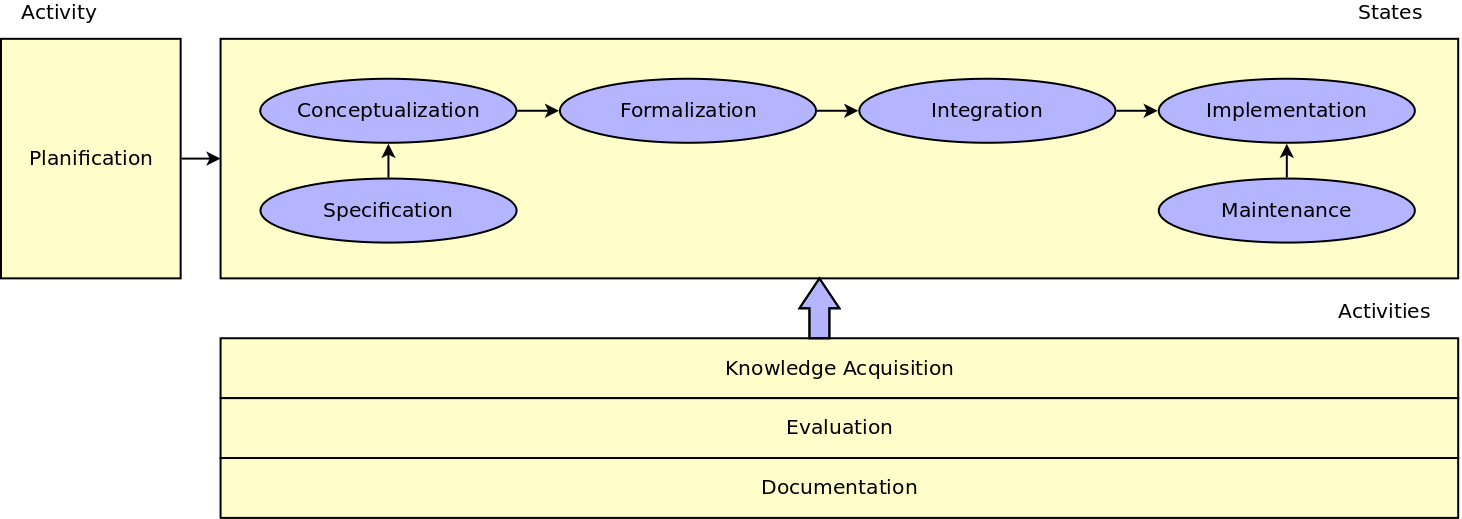
\includegraphics[width=\textwidth]{figures/ontology_lifecycle.pdf}
  \caption{States and activities in the life cycle of an ontology according to \methontology \cite{Methontology}}
  \label{fig:methontology1}
\end{figure}

These activities -- which are depicted in figure \ref{fig:methontology1} -- are arranged into the step of \emph{planification} that must be performed at the very beginning of development, a \emph{set of stages} (consisting of \emph{specification}, \emph{conceptualisation}, \emph{formalisation}, \emph{integration}, \emph{implementation} and \emph{maintenance}) through which the ontology moves during its creation and some activities (\emph{knowledge acquisition}, \emph{documentation} and \emph{evaluation}) that are performed throughout the whole development process in parallel to the stages.

% TODO figure: evolving life-cycle
Differently to what is shown in figure \ref{fig:methontology1}, \methontology follows an evolving life cycle model similar to the iterative-incremental approach that is used in the \emph{Spiral Model} in software development\cite{spiral_model}. This life cycle model which allows the ontology to grow according to its needs. Whenever it is necessary, pieces of the ontology can be added, modified and deleted. Thus, one state does not have to be completely finished before the next state is begun. The ontology cycles through each state numerous times until the ontology meets all requirements and the results of each step correspond to each other.

\subsection{METHONTOLOGY}
\label{sec:methontology}

This section describes \methontology as a well-defined approach to perform all activities mentioned above.

For each of the activities, only ideas behind them are covered, but their application is omitted. They are applied in chapter \ref{ch:smarthomeweather_ontology} where \methontology is used to create the \smarthomeweather ontology.

Each section that describes an activity that involves the creation of some documentation artefact (e.g. a table or a document), a template for the respective artefact is presented.

\subsubsection{Specification}
\label{subsec:methontology_specification}

\methontology defines a precise approach for the development of an ontology. It specifies certain activities that need to be performed, how these activities are performed and in which order. Thus, the activity of \emph{planification} is completed by specifying \methontology itself and the ontology developer is exempted therefrom. Hence, the first step of developing an ontology from scratch is \emph{specification}

During \emph{specification}, an \emph{Ontology Requirements Specification Document} is generated. This document is written in natural language using a set of intermediate representations or using competence questions. It should include

\begin{itemize}
  \item the name and the purpose of the ontology, its scope, its intended uses, and possible end-users,
  \item a list of functional requirements (describing the intended functionality of the ontology) and non-functional requirements (describing all intended properties of the ontology not directly related to its functionality), and
  \item a list of terms that specify the scope of the ontology.
\end{itemize}

A good ontology specification document has the following properties:

Figure~\ref{fig:ontology_specification_template} shows a template of an \emph{Ontology Requirements Specification Document}~\cite{ORSD}.

\begin{figure}
\begin{mdframed}[linewidth=.6pt]
\setlength{\parindent}{0pt}
\MakeUppercase{\textbf{Ontology Requirements Specification Document}}

\textbf{Name}: …

\textbf{Purpose}: …

\textbf{Scope}: …

\textbf{Implementation language}: …

\textbf{Intended end-users}: …

\textbf{Intended uses}: …

\textbf{Ontology requirements}: …

\setlength{\leftskip}{.5cm}

\textbf{Non-functional requirements}: 

\begin{itemize}
  \item …
\end{itemize}

\textbf{Functional requirements}: 

\begin{itemize}
  \item …
\end{itemize}

\setlength{\leftskip}{0cm}

\textbf{Pre-glossary of terms}: …

\end{mdframed}

\caption{Template for the \emph{Ontology Requirements Specification Document} of \methontology~\cite{ORSD}}
\label{fig:ontology_specification_template}
\end{figure}

\subsubsection{Knowledge Acquisition}

Most of knowledge acquisition is done simultanously with the \emph{specification} phase. It is one of the most important activities and needs to be performed thoroughly as most other activities depend heavily on it.

Sources of knowledge are experts, books, handbooks, figures, tables and even other ontologies. Knowledge is collected using techniques such as brainstorming, interviews, formal and informal analysis of texts and knowledge acquisition tools.

\subsubsection{Conceptualisation}
\label{subsec:methontology_conceptualisation}
\begin{figure}
  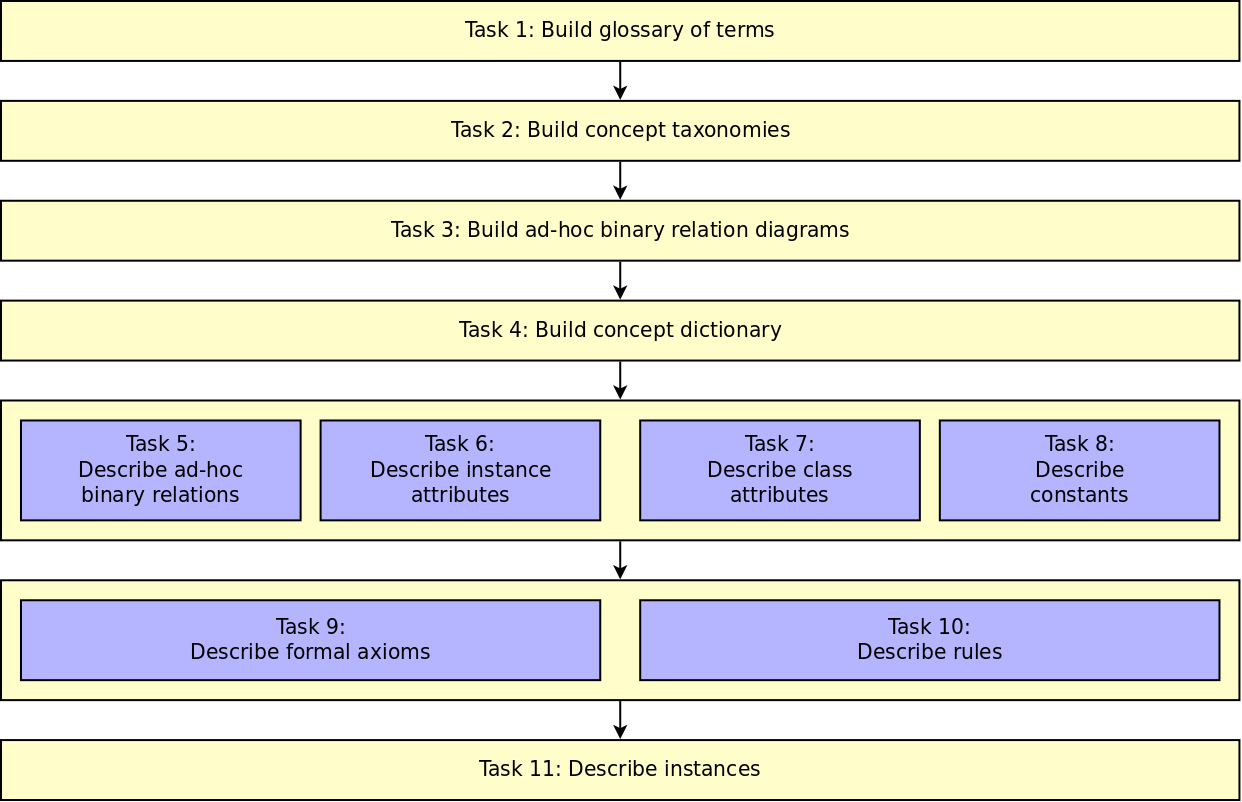
\includegraphics[width=\textwidth]{figures/methontology_tasks.pdf}
  \caption{Tasks of the conceptualisation activity according to \methontology \cite{MethontologyLegal}}
  \label{fig:methontology2}
\end{figure}

The state of \emph{conceptualisation} consists of several tasks as shown in figure \ref{fig:methontology2} \cite{MethontologyLegal}. Again, the figure shows the tasks in a sequential manner. However, as \methontology uses an evolutional process model, the steps is performed numerous times.

% TODO templates for each table
% TODO these sections do not relate to the sections in the next chapter?!
\paragraph{Task 1: Glossary of Terms}

At first, the ontologist builds a \emph{Glossary of Terms}. This glossary includes all the relevant terms of the domain (concepts, instances, attributes, relations etc.). It can be built as a table having the columns \emph{name}, \emph{synonyms}, \emph{acronyms}, \emph{description} (for a natural language description of the term) and \emph{type} (specifying whether the term is a concept, an instance, an attribute, a relation etc.).

\begin{figure}
\centering
\begin{tabular}{|p{.2\textwidth}|p{.2\textwidth}|p{.2\textwidth}|p{.2\textwidth}|}
  \hline
  \textbf{Name} & \textbf{Acronyms} & \textbf{Description} & \textbf{Type} \\
  \hline\hline
  … & … & … & … \\
  \hline
\end{tabular}
\caption{Template for the glossary of terms as proposed by \methontology.}
\label{fig:methontology_example_glossary}
\end{figure}

Figure~\ref{fig:methontology_example_glossary} shows a template for the glossary of terms.

\paragraph{Task 2: Concept Taxonomies}

Once the glossary of terms contains a sizeable number of concepts, these ontologies are arranged in one or more taxonomies that define the concept hierarchy.

\methontology proposes the use of four taxonomic relations:
\begin{enumerate}
  \item \textbf{Subclass-Of}: If a concept $B$ is a \emph{Subclass-Of} a concept $A$, every instance of $B$ is also an instance of $A$.
  \item \textbf{Disjoint-Decomposition}: A \emph{Disjoint-Decomposition} of a concept $C$ is a set of subclasses of $C$ such that an instance of one of these subclasses can never be a subclass of another of these subclasses, while an instance of $C$ is not necessarily an instance of one of its subclasses.
  \item \textbf{Exhaustive-Decomposition}: A \emph{Exhaustive-Decomposition} of a concept $C$ is a set of subclasses of $C$ such that every instance of $C$ is an instance of at least one of its subclasses.
  \item \textbf{Partition}: A \emph{Partition} of $C$ is a set of subclasses of $C$ such that every instance of $C$ is an instance of exactly one of its subclasses.
\end{enumerate}

\begin{figure}
\centering
\includegraphics[width=.9\textwidth]{figures/diagrams/methontology_example_concept_taxonomies.pdf}
\caption{Example of a concept-classification tree as proposed by \methontology.}
\label{fig:methontology_example_concept_taxonomies}
\end{figure}

The concept taxonomies are visualised in \emph{concept-classification trees} which are diagrams that depict the concepts and their taxonomic relations. See figure~\ref{fig:methontology_example_concept_taxonomies} for an example of a concept-classification trees. In case the ontology contains a large number of concepts, the tree may be split into several diagrams in order to keep the trees clear.

\paragraph{Task 3: Ad-hoc binary relation diagrams}

In the next step, \emph{ad-hoc binary relation diagrams} are created. This diagrams show all ad-hoc relationships between concepts of the same (or different) concept taxonomy. See figure~\ref{fig:methontology_example_binary_relations} for an example of a binary relation diagram.

\begin{figure}
\centering
\includegraphics[width=.8\textwidth]{figures/diagrams/methontology_example_binary_relations.pdf}
\caption{Example of a binary relations diagram as proposed by \methontology.}
\label{fig:methontology_example_binary_relations}
\end{figure}

\paragraph{Task 4: Concept dictionary}

The \emph{concept dictionary} contains all domain concepts together with their relations, their instances and their class attributes (i.e. attributes that describe properties of classes) and instance attributes (i.e. attributes that describe properties of instances). All information from the previous steps contribute to this dictionary. The concept dictionary is again being built as a table having appropriate columns for all required information. Like the concept-classification trees, this table may be split into a set of smaller tables if the ontology contains a large number of concepts.

Figure~\ref{fig:methontology_example_concept_dictionary} shows a template for the concept dictionary.

\begin{figure}
\centering
\begin{tabular}{|p{.2\textwidth}|p{.5\textwidth}|p{.2\textwidth}|}
  \hline
  \textbf{Name} & \textbf{Instances} & \textbf{Relations} \\
  \hline\hline
  … & … & … \\
  \hline
\end{tabular}
\caption{Template for the concept dictionary as proposed by \methontology.}
\label{fig:methontology_example_concept_dictionary}
\end{figure}

\paragraph{Task 5: Ad-hoc binary relation details}

In this step, for all ad-hoc binary relations details are specified in a tabular manner. The resulting table has a row for each relation and columns named \emph{relation name}, \emph{source concept}, \emph{source cardinality (max)}, \emph{target concept}, \emph{inverse relation}. Figure~\ref{fig:methontology_example_binary_relations_table} shows a template for the binary relations table.

\begin{figure}
\centering
\begin{tabular}{|p{.167\textwidth}|p{.167\textwidth}|p{.167\textwidth}|p{.167\textwidth}|p{.167\textwidth}|}
  \hline
  \textbf{Name} & \textbf{Source\newline concept} & \textbf{Target\newline concept} & \textbf{Maximum\newline source\newline cardinality} & \textbf{Inverse\newline relation} \\
  \hline\hline
  … & … & … & … & … \\
  \hline
\end{tabular}
\caption{Template for the binary relations table as proposed by \methontology.}
\label{fig:methontology_example_binary_relations_table}
\end{figure}

\paragraph{Task 6: Instance attributes}

This step leads to an \emph{instance attributes table}. That is a table of all \emph{instance attributes} that are listed in the concept dictionary. Each row contains the description of one instance attribute. An instance attribute is an attribute that describes a property of an instance of a concept. Its value may be different for each instance of the concept.

The columns of the table are \emph{attribute name}, \emph{concept name}, \emph{value type} (\emph{Integer}, \emph{Float}, \emph{String}, etc.), \emph{value range}, \emph{minimum cardinality} and \emph{maximum cardinality}. Additionally, the following information may be specified: instance attributes, class attributes and constants used to infer values of the attribute; attributes that can be inferred using values of this attribute; formulae or rules that allow inferring values of the attribute; and references used to define the attribute.

See figure~\ref{fig:methontology_example_instance_attributes} for a template for the instance attributes table.

\begin{figure}
\centering
\begin{tabular}{|p{0.15\textwidth}|p{0.15\textwidth}|p{0.15\textwidth}|p{0.15\textwidth}|p{0.15\textwidth}|p{0.15\textwidth}|}
  \hline
  \textbf{Attribute name} & \textbf{Concept name} & \textbf{Value type} & \textbf{Value range} & \textbf{Unit} & \textbf{Cardinality} (min, max)\\
  \hline\hline
  … & … & … & … & … & … \\
  \hline
\end{tabular}
\caption{Template for the instance attributes table as proposed by \methontology.}
\label{fig:methontology_example_instance_attributes}
\end{figure}

\paragraph{Task 7: Class attributes}

All class attributes that are listed in the concept dictionary are described in detail in the \emph{class attributes table}. Each row describes one class attribute. The columns are \emph{name}, \emph{concept name} (i.e. the name of the concept where the attribute is defined), \emph{value type}, \emph{value(s)}, \emph{minimum cardinality} and \emph{maximum cardinality}. Additionally, all information about related instance attributes, class attributes, constants, rules, and formulae may be specified that are specified in the instance attribute as well.

\begin{figure}
\centering
\begin{tabular}{|p{0.22\textwidth}|p{0.22\textwidth}|p{0.22\textwidth}|p{0.22\textwidth}|}
  \hline
  \textbf{Super-concept} & \textbf{Sub-concept} & \textbf{attribute name} & \textbf{attribute value(s)} \\
  \hline\hline
  … & … & … & … \\
  \hline
\end{tabular}
\caption{Template for the class attributes table as proposed by \methontology.}
\label{fig:methontology_example_class_attributes}
\end{figure}

Figure~\ref{fig:methontology_example_class_attributes} shows a template for the class attributes table.

\paragraph{Task 8: Constants}

In this step, the \emph{constants table} is created that specifies details about all the constants listed in the glossary of terms. For each constant is specified by its name, its value type, its value, the measurement unit for numerical constants, and the attributes that can be inferred using the constant.

% TODO constants table -> instances table?
\begin{figure}
\centering
\begin{tabular}{|p{0.2\textwidth}|p{0.2\textwidth}|}
  \hline
  \textbf{Instance name} & \textbf{Concept name} \\
  \hline\hline
  … & … \\
  \hline
\end{tabular}
\caption{Template for the constants table as proposed by \methontology.}
\label{fig:methontology_example_constants}
\end{figure}

Figure~\ref{fig:methontology_example_constants} shows a template for the constants table.

\paragraph{Task 9: Formal axioms}

% TODO

% TODO template

\paragraph{Task 10: Rules}

% TODO

% TODO template

\paragraph{Task 11: Instances}

% TODO

\subsubsection{Formalisation}

\emph{Formalisation} is the transition from the informal description from the tables and diagrams in the previous step of \emph{conceptualisation} into the chosen ontology language, e.g. \eacs{OWL}. As this is tightly coupled with the \emph{implementation} of the ontology (see section~\ref{subsec:methontology_implementation}), this is a task which is not performed described separately.

\subsubsection{Integration}

As ontologies are built for reuse and the wheel shall not be reinvented during the creation of a new ontology, the ontology designer searches for existing ontologies. The goal is to import ontologies that already define terms that are part of the conceptualisation of the ontology currently being developed.

\subsubsection{Implementation}
\label{subsec:methontology_implementation}

The task of implementing the ontology in an ontology language requires an environment that supports the ontologies selected in the integration step. Features that should be provided by such an environment are~\cite{Methontology}

\begin{itemize}
  \item a lexical and syntactic analyser to guarantee the absence of lexical and syntactic errors,
  \item an editor for adding, modifying and removing definitions,
  \item a browser for inspecting the library of ontologies and their definitions,
  \item a searcher for looking for the most appropriate definitions,
  \item evaluators for detecting incompleteness, inconsistencies and redundant knowledge and
  \item an automatic maintainer for managing the inclusion, removal or modification of existing definitions.
\end{itemize}

Together with the implementation, the information about the ontology gathered in section~\ref{subsec:methontology_conceptualisation} is now formalised into the formal model of the ontology language being used.

In the case of the \smarthomeweather ontology an \eacs{OWL} ontology~\cite{OWL} is created using \protege~\cite{protege} together with the \emph{Pellet} reasoner~\cite{pellet}.

\subsubsection{Evaluation}

During \emph{Evaluation}, verification takes place whether all artefacts that have yet been created or updated in the previous steps satisfy the requirements that have been specified initially (see section~\ref{subsec:methontology_specification}). \emph{Evaluation} is not an activity which is performed at the very end of the development process; instead, \emph{Evaluation} takes place whenever an artefact (a diagram, a table, or the implementation of the ontology) is created or updated in order to ensure that mistakes are found as soon as possible.

The completed ontology must fulfil all functional and non-functional requirements listed the \emph{Ontology Requirements Specification Document} presented in section~\ref{subsec:methontology_specification}. In case of a mismatch, the ontology traverses the activities in the life cycle (\emph{Conceptualisation}, \emph{Formalisation}, \emph{Integration}, \emph{Implementation}, and \emph{Evaluation}) once more.

There may be requirements that an ontology is unable to fulfil due to certain limitations, e.g. the \emph{open world assumption}~\cite{open_world_assumption1}. For instance, \eacs{OWL}, which honors the \emph{open world assumption}, cannot tell the absence of an instance of some concept. This leads to cases where an ontology fails to answer a competency question such as ``Does this group only consist of women?''; just because the ontology does not contain an individual which is a man, it does not mean that there is no man; the ontology can only tell that there is no man it knows about.

Evaluation (and specification) must take limitations into account which affect ontologies generally or the ontology language being used.

\subsubsection{Documentation}

During the steps described above, a set of documents is compiled. If generated properly and accurately, these documents describe every detail of the ontology. Using this approach, \methontology forces the ontology designer to document throughout the development process. Any problems that come with documentation being created after the development process -- e.g. incomplete or wrong documentation, the ontology designer does not write the documentation herself, or some ideas the designer had in the design process are lost~\cite{SoftwareDocumentationProblems} -- are avoided.

Hence, in \methontology, \emph{documentation} is an activity that is not performed explicitly. Once the development process has finished, both the ontology and its documentation are ready to use. 

\subsubsection{Maintenance}

At any time in the future, changes to the ontology may become necessary. A modification of the ontology's requirements may be one reason therefor; inaccurateness that occurs during the ontology development process may be another reason.

Whenever a change is necessary, the ontology again cycles the states of \emph{specification}, \emph{conceptualisation}, \emph{formalisation}, \emph{integration} and \emph{implementation} repeatedly until all requirements are met and all artefacts generated in these states correspond to each other. \emph{Knowledge acquisition} and \emph{evaluation} are again performed throughout all of these states.



% TODO acronyms

\chapter{The \thinkhomeweather ontology}
\label{ch:thinkhomeweather_ontology}


% TODO check if the things mentioned here are properly covered in the chapters referred

% TODO elaborate steps more?


The previous chapters cover all topics that require discussion before being able to build a new ontology from scratch: Chapter \ref{ch:weather_data} discusses all details about weather data that is necessary and reasonable for the \thinkhomeweather ontology, what data will be used and where to obtain it. Chapter \ref{ch:existing_work} gives an overview about existing ontologies in the domain of weather data. As none of the existing ontologies being discussed fits the needs of an ontology for \thinkhome, a new ontology is to be designed. Chapter \ref{ch:development_approaches} analyses some of the most popular approaches for building ontologies from scratch. Among those, \methontology \cite{Methontology} is identified to be the best suitable approach.

Based on these insights, this chapter describes the process of designing the \thinkhomeweather ontology in detail. The development process follows the steps proposed by \methontology as described in chapter \ref{sec:methontology}.

\section{Conventions}
\label{sec:ontology_conventions}

\begin{figure}
  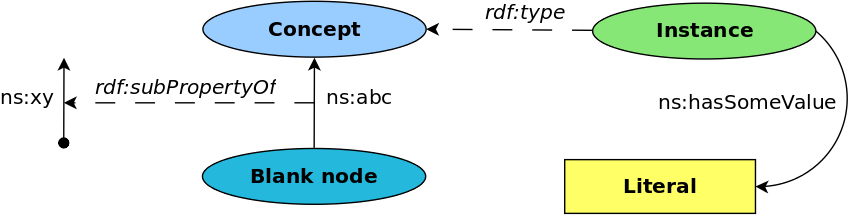
\includegraphics[width=\textwidth]{figures/diagrams/template.pdf}
  \caption{Example diagram}
  \label{fig:diagram_example}
\end{figure}

\definecolor{convention_color1}{HTML}{99CCFF}
\definecolor{convention_color2}{HTML}{87E776}
\definecolor{convention_color3}{HTML}{23B8DC}
\definecolor{convention_color4}{HTML}{FFFF66}
\definecolor{convention_color_bg4}{HTML}{AAAAAA}

All diagrams in this chapter showing parts of an ontology adhere to the following conventions, as seen in the example diagram shown in figure \ref{fig:diagram_example}:
\begin{itemize}
  \item \emph{Concepts} are drawn as ellipses filled with the color \texttt{\textcolor{convention_color1}{\#99CCFF}}.
  \item \emph{Instances} are drawn as ellipses filled with the color \texttt{\textcolor{convention_color2}{\#87E776}}.
  \item \emph{Blank nodes} are drawn as ellipses filled with the color \texttt{\textcolor{convention_color3}{\#23B8DC}}.
  \item \emph{Literals} are drawn as rectangles filled with the color \texttt{\colorbox{convention_color_bg4}{\textcolor{convention_color4}{\#FFFF66}}}.
  \item \emph{Properties in the RDF\cite{RDF} and RDFS\cite{RDFS} namespace} are drawn as dashed lines. Their caption is written in \emph{italics}.
  \item \emph{Properties in other namespaces} are drawn as solid lines. Their caption is \emph{not} written in \emph{italics}.
\end{itemize}

Every ontology should stick to a set of naming conventions that are explicitly stated \cite{Ontology101}. The conventions for \thinkhomeweather are as follows:

\begin{itemize}
  \item Two concepts, instances and/or properties may not have the same identifier as this is required by \emph{OWL}\cite{OWL}\footnote{Using one identifier for more than one concept, instance and properties is possible in \emph{OWL} if an adequate number of namespaces is used. However, \thinkhomeweather uses a single namespace.} and avoids confusion.
  \item Two identifiers may not use names that only differ in their capitalization. Using both \emph{Weather State} and \emph{weather state} in the name namespace is possible in \emph{OWL}, but leads to confusion.
  \item Identifiers may only consist of upper and lower case ASCII letters (\emph{A} to \emph{Z} and \emph{a} to \emph{z}), numerical digits from \emph{0} to \emph{9} and spaces, i.e. all identifiers must match the regular expression \texttt{\textasciicircum[A-za-z0-9~]+\$}.
  \item \emph{Concepts} have an identifier that is in singular case and starts with an upper case letter. Typically a concept's identifier is a noun, e.g. \emph{Weather state} or \emph{Weather report}.
  \item \emph{Properties} have an identifier that starts with a lower case letter and starts with the prefix \emph{has} or \emph{belongs to}, followed by the name of the name of the concept which is the property's \emph{range}. The inverse property of a property having an identifier starting with \emph{has} has an identifier starting with \emph{belongs to}, followed by the inverse property's \emph{range}, and vice versa. As an alternative to the prefix \emph{belongs to}, the prefix \emph{is} in conjunction with the suffix \emph{of} and the inverse property's \emph{domain} may be used.
  
  E.g. the name of a property with the domain \emph{Weather report} and the range \emph{Weather state} has the name \emph{has weather state}. If \emph{has weather state} has an inverse property, it will have the name \emph{belongs to weather report} or \emph{is weather state of}.
\end{itemize}


\section{Specification}
\label{sec:ontology_specification}

\emph{Specification}, the first step proposed by \methontology, aims at creating an \emph{Ontology Requirements Specification Document} using natural language. It adheres to the approach discussed in chapter \ref{sec:methontology} and uses the document template taken from \cite{ORSD}.

\vspace{1em}

% TODO ensure there are no problematic page breaks inside this box (e.g. between the headline 'Scope:' and the first bullet point)
\begin{mdframed}[linewidth=.6pt]
\setlength{\parindent}{0pt}
\vspace{.4cm}

\MakeUppercase{\textbf{Ontology Requirements Specification Document}}

\vspace{.6cm}

\textbf{Name}: \thinkhomeweather

\vspace{.3cm}

\textbf{Purpose}: The ontology covers data about weather phenomena occurring at a certain location somewhere on Earth between the present and 24 hours in the future. Weather data will be acquired from both Internet services as well as from weather sensors mounted at the desired location. This weather data will enable the \thinkhome system to make decisions based on current and future weather conditions.

\vspace{.3cm}

\textbf{Scope}: The ontology has to cover a set of five core concepts from the domain of weather data:

\begin{itemize}
  \item \emph{weather phenomenon}: Represents a certain weather element. Relevant weather elements are \emph{temperature}, \emph{humidity}, \emph{dew point}, \emph{wind speed} and \emph{direction}, \emph{precipitation intensity} and \emph{probability}, \emph{atmospheric pressure}, \emph{cloud cover}, \emph{solar radiation}, and the \emph{sun's position}.
  \item \emph{Weather condition}: Overall state of the weather given by a simple verbal description: \emph{sun}, \emph{light clouds}, \emph{partly cloudy}, \emph{cloudy}, \emph{fog}, \emph{rain}, \emph{snow}, \emph{sleet}, \emph{thunder}.
  \item \emph{Weather state}: Summarizes all weather phenomena for a certain time. 
  \item \emph{Weather report}: Summarizes all data acquired at a certain time about the current weather or the weather some time in the future. Exactly one \emph{weather state} is linked to each \emph{weather report}.
  \item \emph{Weather report source}: Source where the data belonging to a \emph{weather report} has been obtained from (either an Internet weather service or a local weather sensor).
\end{itemize}

\vspace{.3cm}

\textbf{Implementation language}: The ontology is implemented in \emph{OWL 2.0}\cite{OWL} using \protege\footnote{\href{http://protege.stanford.edu/}{http://protege.stanford.edu/}} and the \emph{Pellet reasoner}\footnote{\href{http://clarkparsia.com/pellet/}{http://clarkparsia.com/pellet/}}.

\vspace{.3cm}

\textbf{Intended end-users}: The ontology is part of the \thinkhome project; hence, any end-user of the \thinkhome project is an end-user of the \thinkhomeweather ontology. As \thinkhome aims at providing home automation to \emph{house occupants}, intended end-users of \thinkhomeweather are these occupants.

\vspace{.3cm}

\textbf{Intended uses}: The ontology shall provide knowledge to \thinkhome about the current and future state of the weather in order to enable \thinkhome to make decisions based on that knowledge.

% TODO re-add this vspace?
\vspace{.3cm}

\textbf{Ontology requirements}:

\vspace{.3cm}

\setlength{\leftskip}{.5cm}

\textbf{Non-functional requirements}:

\begin{itemize}
  \item The ontology must adhere to the naming conventions presented in section \ref{sec:ontology_conventions} regarding the identifiers that may be used for classes, properties and individuals.
  \item The ontology must be documented thoroughly in order to make it easily reusable.
  \item The ontology must re-use existing ontologies wherever possible.
\end{itemize}

\textbf{Functional requirements}: The functional requirements are covered by the competency questions that the ontology shall be able to answer (see section \ref{sec:weather_information}):

\begin{itemize}
  \item What is the current weather situation?
  \item What will the weather situation be in one hour, in two hours, …, in 24 hours?
  \item What is the current temperature, humidity, wind speed, …?
  \item What will be the temperature, humidity, wind speed, … in one hour, in two hours, …, in 24 hours?
  \item What will be the minimum temperature, humidity, … over the next 24 hours? What about maximum values?
  \item Will the weather change? Will the temperature, humidity, … rise or fall?
  \item Does it rain? Will it rain in the next hours? Will it rain today?
  \item Will there be sunshine today? 
  \item Do we need to irrigate the garden?
  \item Will there be severe weather?
  \item Will temperature drop/stay below $0^\circ C$?
  \item When can we open windows and when do we have to keep them shut?
  \item When do we need sun protection?
  \item When will it outside be colder than inside the house? When will it be warmer?
\end{itemize}

\setlength{\leftskip}{0cm}

\vspace{.2cm}

\textbf{Pre-glossary of terms}: These are all terms that can be extracted from the competency questions, in alphabetical order:

24 hours, airing, current weather, frost, future weather, humidity, humidity rise, humidity fall, irrigation, minimum, maximum, rain, room temperature, severe weather, sunshine, sun protection, temperature, temperature rise, temperature fall, weather change, wind speed.

\setlength{\leftskip}{0cm}

\end{mdframed}

\vspace{.5cm}

In the following sections, the \thinkhomeweather ontology is built in a way to meet all above requirements, if possible. Section \ref{sec:ontology_evaluation} evaluates if the resulting ontology fits the specification and which shortcomings the ontology comes with.

\section{Knowledge Acquisition}

The second step proposed by \methontology is \emph{Knowledge Acquisition}. All knowledge required to build the \thinkhomeweather ontology is presented in the chapters~\ref{ch:existing_work} and~\ref{ch:weather_data}. These chapters discuss in detail:

\begin{itemize}
  \item Which weather data are relevant for \thinkhome?
  \item Which weather data are available from sensors (section~\ref{sec:weather_sensors}) and Internet services (section~\ref{sec:internet_services})? How can this data be acquired?
  \item Which data do not have any use for \thinkhomeweather due to being too complicated or because they cannot be processed in an ontology in a useful way?
  \item What knowledge about weather in general is required to build an appropriate ontology? % TODO check if this is available in the previous chapters
\end{itemize}

Furthermore, chapter~\ref{ch:existing_work} covers existing ontologies that cover the domain of weather data. An additional source of knowledge is available through works about weather in general, e.g. the \emph{Glossary of Meteorology}\footnote{\href{http://glossary.ametsoc.org/wiki/Main\_Page}{http://glossary.ametsoc.org/wiki/Main\_Page}} by the \emph{American Meteorological Society}\footnote{\href{http://www.ametsoc.org/}{http://www.ametsoc.org/}}\cite{GlossaryOfMeteorology}.

\section{Conceptualisation}
\label{sec:ontology_concept}

In the third step of \methontology, the \emph{Conceptualisation} step, the domain knowledge is structured into a conceptional model that describes the problem and its solution in terms of the domain vocabulary that has been identified in the \emph{Specification} process.

The starting point of \emph{Conceptualisation} is a complete \emph{Glossary of Terms} that covers all concepts, instances, attributes and binary relations that will form the ontology. Besides the glossary, this section covers \emph{Concept-classification trees} (section~\ref{sec:concept_classification_trees}), \emph{Binary relationship diagrams} (section~\ref{subsec:binary_relations_diagram}), \emph{Concept dictionaries} (section~\ref{subsec:binary_relations_diagram}), \emph{Binary relations tables} (section~\ref{subsec:binary_relations_table}), \emph{Instance attribute tables} (section~\ref{subsec:binary_relations_table}) and \emph{Class attributes tables} (section~\ref{subsec:class_attributes_table}). \emph{Constant tables}, \emph{Formal axiom tables} and \emph{Rules tables} have been omitted as the components described by these tables do not appear in \thinkhomeweather.

In this section, only those deliverables are presented that are necessary to fully understand the structure of \thinkhomeweather. All tables that have only been created for the sake of completeness can be found in appendix~\ref{sec:appendix_conceptualisation}.

\subsection{Glossary of Terms}
\label{sec:ontology_glossary}

When describing the scope of \thinkhomeweather, the \emph{Ontology Requirements Specification Document} in section~\ref{sec:ontology_specification} mentions five top-level concepts (i.e. concepts that do not have a superclass except \emph{Thing} in \emph{OWL}) of the ontology: \Egls{weather report}, \Egls{weather state}, \Egls{weather phenomenon}, and \Egls{weather condition}. All other concepts are sub-concepts of these five concepts.

In this section, only a list of terms is given; the complete \emph{Glossary of Terms} with short descriptions of each term can be found in the appendix~\ref{main} which starts on page~\pageref{main}.

\paragraph{Concepts:}

% TODO link to section/subsection?
Section~\ref{ch:weather_data} discusses each weather element that is used in \thinkhomeweather and categories in which its instances can be grouped into. In the ontology, all weather elements are represented by concepts that sub-concepts of \Egls{weather phenomenon}. All categories of weather elements are in turn sub-concepts of the weather elements' concepts.

A \egls{weather report} can encapsulate data either about the current weather or about the weather some time in the future which is specified by its \egls{start time}. Additionally, weather data can origin at a set of weather sensors or at an Internet weather service. To take this into account, a few sub-concepts of \egls{weather report} are introduced:

If the \egls{weather report} describes the current weather, it is a \Egls{current weather report}; if it describes the future weather, it is a \Egls{forecast weather report}. Depending on how far the \Egls{weather report}'s \egls{start time} lies ahead, it is a \Egls{short range weather report} (at most 3 hours in the future), a \Egls{medium range weather report} (more than 3 hours and less than 12 hours in the future) or a \Egls{long range weather report} (at least 12 hours in the future). Furthermore, there are sub-concepts of \egls{weather report}, each having a \egls{start time} of 1, 2, 3, 6, 9, 12, 15, 18, or 24 hours; these concepts are named \emph{Forecast 1 hour weather report}, \emph{Forecast 2 hours weather report} etc., respectively.

If the source of weather data is a \Egls{sensor source}, the corresponding \Egls{weather report} is a \Egls{weather report from sensor}; otherwise (if the source of weather data is a \Egls{service source}), it is a \Egls{weather report from service}.

A \Egls{weather report} that is both a \Egls{current weather report} and a \Egls{weather report from sensor} is a \Egls{current weather report from sensor}. A \Egls{weather report} that is both a \Egls{current weather report} and a \Egls{weather report from service} is a \Egls{current weather report from service}.

Several sub-concepts of \Egls{weather state} describe certain combinations of instances of \Egls{weather phenomenon} being associated with a \Egls{weather state}. These concepts are listed below; refer to the glossary in appendix~\ref{main} for their definitions.

Hence, these are the concepts that can be found in \thinkhomeweather are:
\begin{itemize}
  \item \Egls{weather condition}
  \item \Egls{weather phenomenon}:
    \begin{itemize}
      \item \Egls{atmospheric pressure}: \Egls{very low pressure}, \Egls{low pressure}, \Egls{average pressure}, \Egls{high pressure}, \Egls{very high pressure}
      \item \Egls{cloud cover}: \Egls{clear sky}, \Egls{partly cloudy}, \Egls{mostly cloudy}, \Egls{overcast}, \Egls{unknown cloud cover}.
      \item \Egls{dew point}.
      \item \Egls{humidity}: \Egls{very dry}, \Egls{dry}, \Egls{normal humidity}, \Egls{moist}, \Egls{very moist}.
      \item \Egls{precipitation}: \Egls{no rain}, \Egls{light rain}, \Egls{medium rain}, \Egls{heavy rain}, \Egls{extremely heavy rain}, \Egls{tropical storm rain}.
      \item \Egls{solar radiation}: \Egls{no radiation}, \Egls{low radiation}, \Egls{medium radiation}, \Egls{high radiation}, \Egls{very high radiation}.
      \item \Egls{sun position}: \Egls{day}, \Egls{solar twilight}, \Egls{sun below horizon}, \Egls{twilight}, \Egls{civil twilight}, \Egls{nautical twilight}, \Egls{astronomical twilight}, \Egls{night}, \Egls{sun from north}, \Egls{sun from east}, \Egls{sun from south}, \Egls{sun from west}.
      \item \Egls{temperature}: \Egls{frost}, \Egls{cold}, \Egls{below room temperature}, \Egls{room temperature}, \Egls{above room temperature}, \Egls{heat}.
      \item \Egls{wind}: \Egls{directional wind}, \Egls{north wind}, \Egls{east wind}, \Egls{south wind}, \Egls{west wind}, \Egls{calm}, \Egls{light wind}, \Egls{strong wind}, \Egls{storm}, \Egls{hurricane}.
    \end{itemize}
  \item \Egls{weather report}: \Egls{weather report from sensor}, \Egls{weather report from service}, \Egls{current weather report}, \Egls{current weather report from sensor}, \Egls{current weather report from service}, \Egls{forecast weather report}, \Egls{short range weather report}, \Egls{medium range weather report}, \Egls{long range weather report}, \emph{Forecast 1 hour weather report}, \emph{Forecast 2 hours weather report}, …, \emph{Forecast 24 hours weather report}
  \item \Egls{weather source}: \Egls{sensor source}, \Egls{service source}.
  \item \Egls{weather state}: \egls{airing weather}, \egls{calm weather}, \egls{clear weather}, \egls{cloudy weather}, \egls{cold weather}, \egls{dry weather}, \egls{fair weather}, \egls{hot weather}, \egls{moist weather}, \egls{no rain weather}, \egls{pleasant temperature weather}, \egls{rainy weather}, \egls{severe weather}, \egls{sun protection weather}, \egls{thunderstorm}, \egls{very rainy weather}, \egls{windy weather}
\end{itemize}

\paragraph{Relations:}

Instances of the concepts are associated to each other with binary relations, which are:

\begin{itemize}
  \item \egls{has source} and \egls{is source of} which connect instances of \Egls{weather report} and \Egls{weather source}.
  \item \egls{has weather state} and \egls{belongs to weather report} which connect instances of \Egls{weather report} and \Egls{weather state}.
  \item \egls{has condition} which connects instances of \Egls{weather state} and \Egls{weather condition}.
  \item \egls{has weather phenomenon} and \egls{belongs to state} which connect instances of \Egls{weather state} and \Egls{weather phenomenon}.
  \item \egls{has previous weather state} and \egls{has next weather state} which connect two instances of \Egls{weather state}.
\end{itemize}

The following relations link instances of concepts from other ontologies than \thinkhomeweather to instances of concepts inside the ontology: \egls{has start time}, \egls{has end time}, \egls{has observation time}, and \egls{location}.

The only data property in \thinkhomeweather is \egls{has priority} which specifies an integer value indicating which \Egls{weather report} for a certain period of time is to be preferred over another \Egls{weather report} for the same period of time.

\paragraph{Individuals:}

The only predefined individuals are instances of the concept \Egls{weather condition}; they represent the overall state of the weather for a certain \Egls{weather state}. These individuals are: \emph{cloud}, \emph{fog}, \emph{light clouds}, \emph{partly cloudy}, \emph{rain}, \emph{sleet}, \emph{snow}, \emph{sun}, and \emph{thunder}.

\subsection{Concept-classification trees}
\label{sec:concept_classification_trees}

As stated in section~\ref{sec:ontology_glossary}, there are fix top-level concepts; all other concepts are sub-concepts to these top-level concepts. As a consequence, each of these concepts becomes root of a tree of concepts. These \emph{Concept-classification trees} are presented in this section.

A \Egls{weather condition} does not have any sub-concepts. Hence, its classification tree which is shown in figure~\ref{fig:tree_weather_condition} looks rather simple.

\begin{figure}
  \centering
  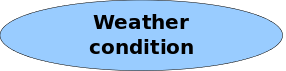
\includegraphics[width=.3\textwidth]{figures/diagrams/weather-condition.pdf}
  \caption{Concept-classification tree for \Egls{weather condition}}
  \label{fig:tree_weather_condition}
\end{figure}

A \Egls{weather phenomenon} represents a certain weather element. Every specific weather element is a sub-concept of \Egls{weather phenomenon}; the evolving tree is shown in~\ref{fig:tree_weather_phenomenon}. For sake of clarity, this tree is broken up to several diagrams; all sub-concepts of sub-concepts of \Egls{weather phenomenon} are not shown in~\ref{fig:tree_weather_phenomenon}. There is a separate diagram for each sub-concept of \Egls{weather phenomenon}: \Egls{atmospheric pressure} (figure~\ref{fig:tree_atmospheric_pressure}), \Egls{cloud cover} (figure~\ref{fig:tree_cloud_cover}), \Egls{humidity} (figure~\ref{fig:tree_humidity}), \Egls{precipitation} (figure~\ref{fig:tree_precipitation}), \Egls{solar radiation} (figure~\ref{fig:tree_solar_radiation}), \Egls{sun position} (figure~\ref{fig:tree_sun_position}), \Egls{temperature} (figure~\ref{fig:tree_temperature}), and \Egls{wind} (figure~\ref{fig:tree_wind}). The diagram for \Egls{dew point} is not shown as that concept does not have any sub-concepts;
 hence its concept-classification tree consists of a single node.

\begin{figure}
  \centering
  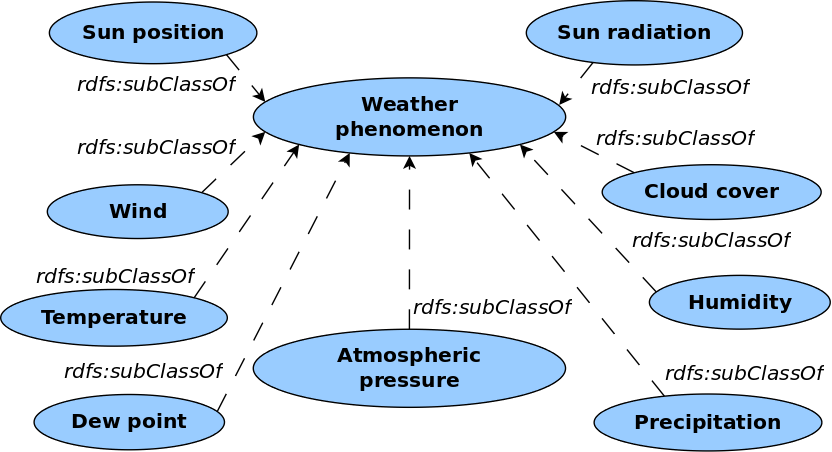
\includegraphics[width=.8\textwidth]{figures/diagrams/weather-phenomenon.pdf}
  \caption{Concept-classification tree for \Egls{weather phenomenon}}
  \label{fig:tree_weather_phenomenon}
\end{figure}

\begin{figure}
  \centering
  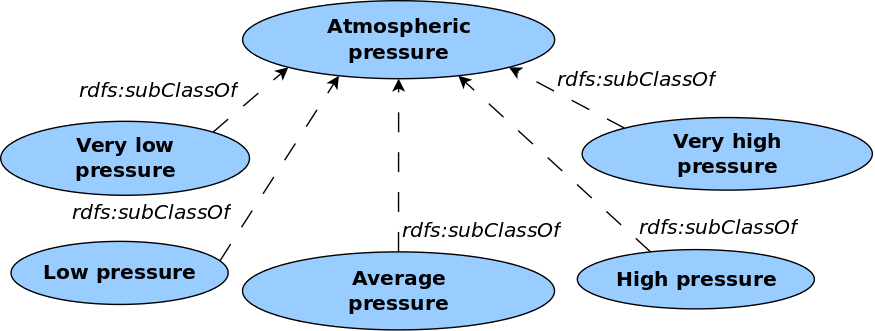
\includegraphics[width=.8\textwidth]{figures/diagrams/atmospheric-pressure.pdf}
  \caption{Concept-classification tree for \Egls{atmospheric pressure}}
  \label{fig:tree_atmospheric_pressure}
\end{figure}

\begin{figure}
  \centering
  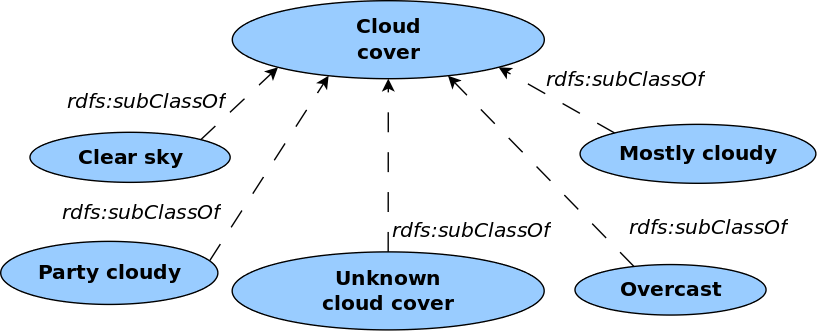
\includegraphics[width=.8\textwidth]{figures/diagrams/cloud-cover.pdf}
  \caption{Concept-classification tree for \Egls{cloud cover}}
  \label{fig:tree_cloud_cover}
\end{figure}

\begin{figure}
  \centering
  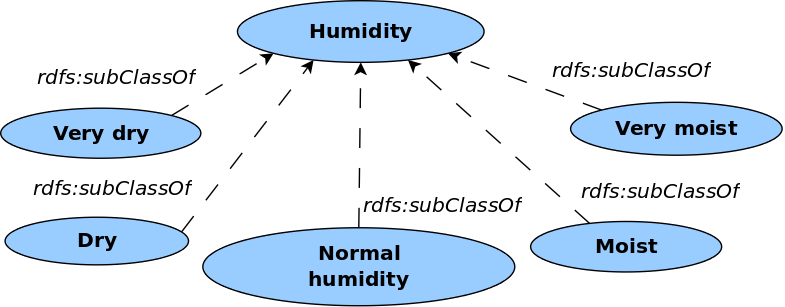
\includegraphics[width=.8\textwidth]{figures/diagrams/humidity.pdf}
  \caption{Concept-classification tree for \Egls{humidity}}
  \label{fig:tree_humidity}
\end{figure}

\begin{figure}
  \centering
  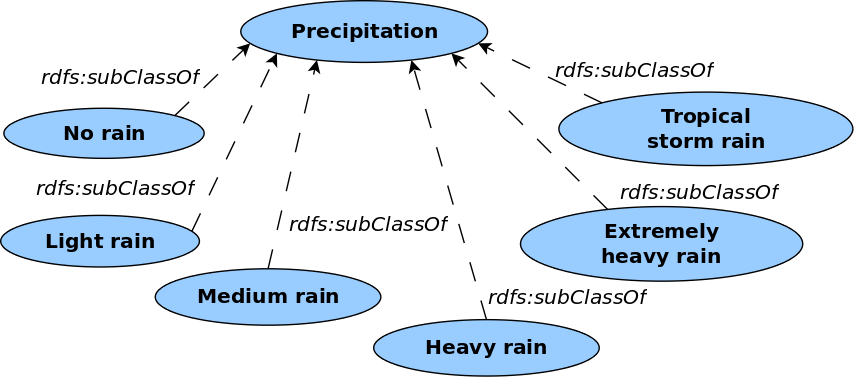
\includegraphics[width=.8\textwidth]{figures/diagrams/precipitation.pdf}
  \caption{Concept-classification tree for \Egls{precipitation}}
  \label{fig:tree_precipitation}
\end{figure}

\begin{figure}
  \centering
  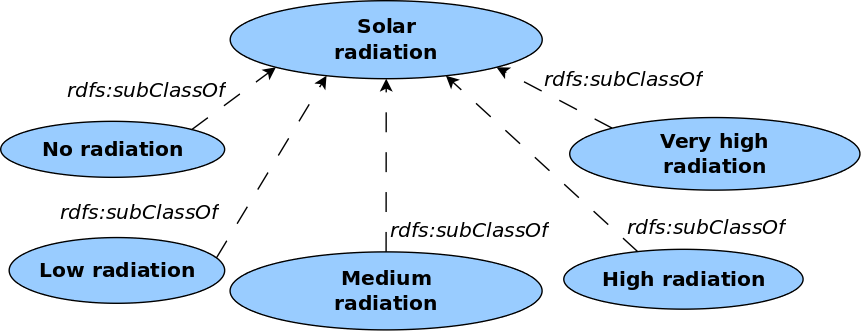
\includegraphics[width=.8\textwidth]{figures/diagrams/solar-radiation.pdf}
  \caption{Concept-classification tree for \Egls{solar radiation}}
  \label{fig:tree_solar_radiation}
\end{figure}

\begin{figure}
  \centering
  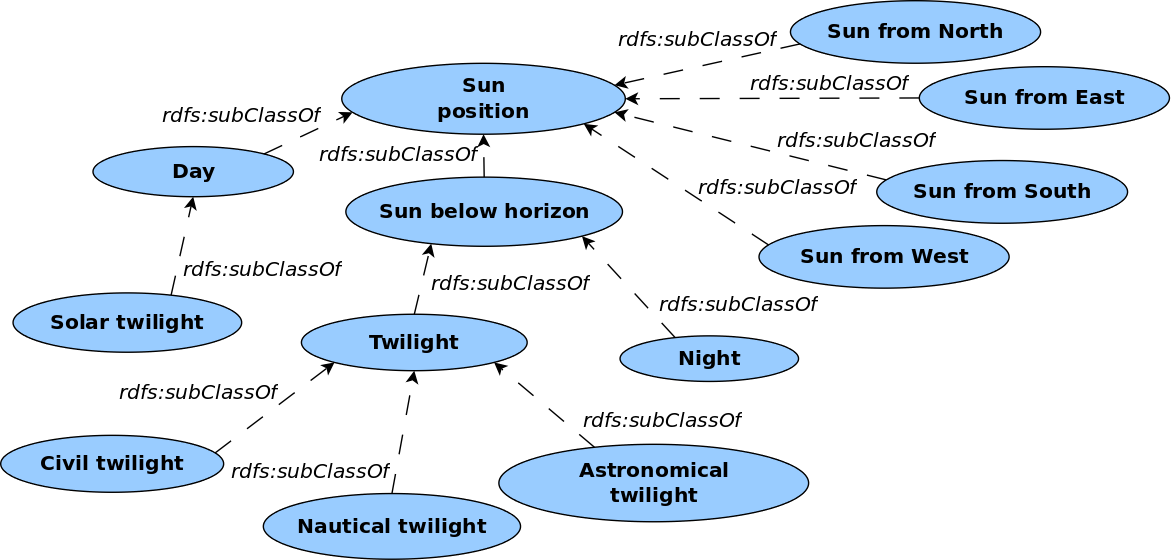
\includegraphics[width=\textwidth]{figures/diagrams/sun-position.pdf}
  \caption{Concept-classification tree for \Egls{sun position}}
  \label{fig:tree_sun_position}
\end{figure}

\begin{figure}
  \centering
  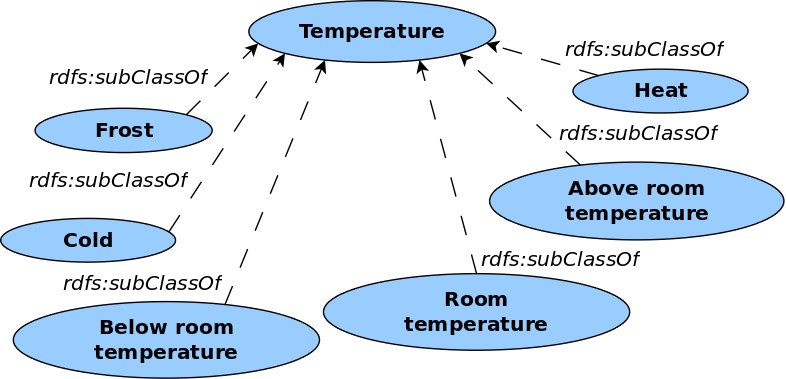
\includegraphics[width=.8\textwidth]{figures/diagrams/temperature.pdf}
  \caption{Concept-classification tree for \Egls{temperature}}
  \label{fig:tree_temperature}
\end{figure}

\begin{figure}
  \centering
  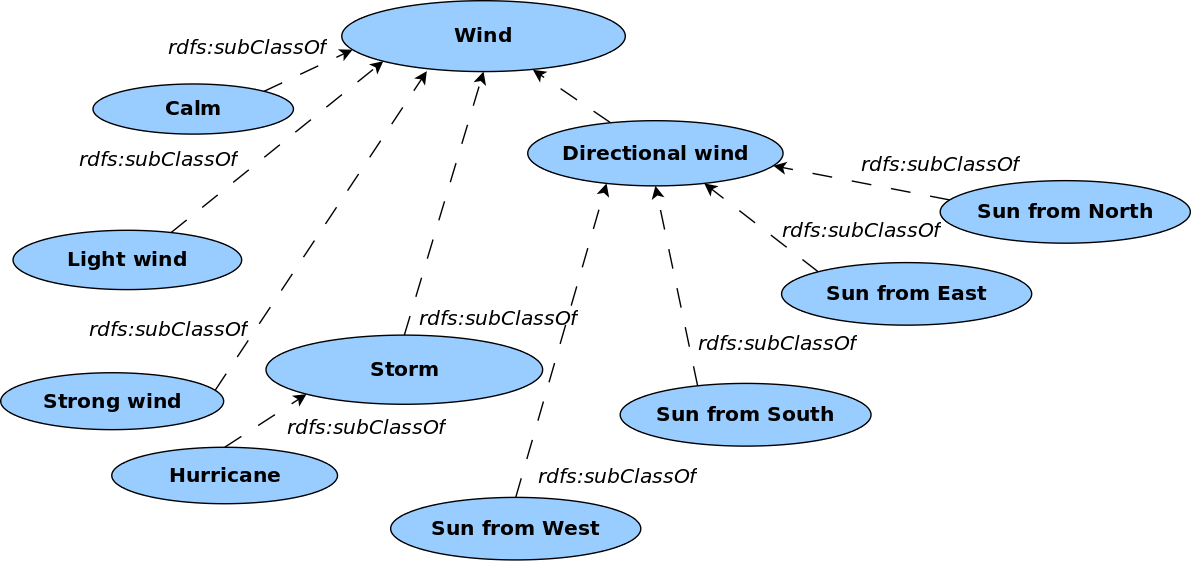
\includegraphics[width=\textwidth]{figures/diagrams/wind.pdf}
  \caption{Concept-classification tree for \Egls{wind}}
  \label{fig:tree_wind}
\end{figure}

A \Egls{weather report} has two attributes that define its main characteristics: \egls{has start time} and \egls{has source}. As discussed in section~\ref{sec:ontology_glossary}, a number of sub-concepts is defined in order to reflect different values of these two attributes. The resulting concept-classification tree is shown in figure~\ref{fig:tree_weather_report}.

\begin{figure}
  \centering
  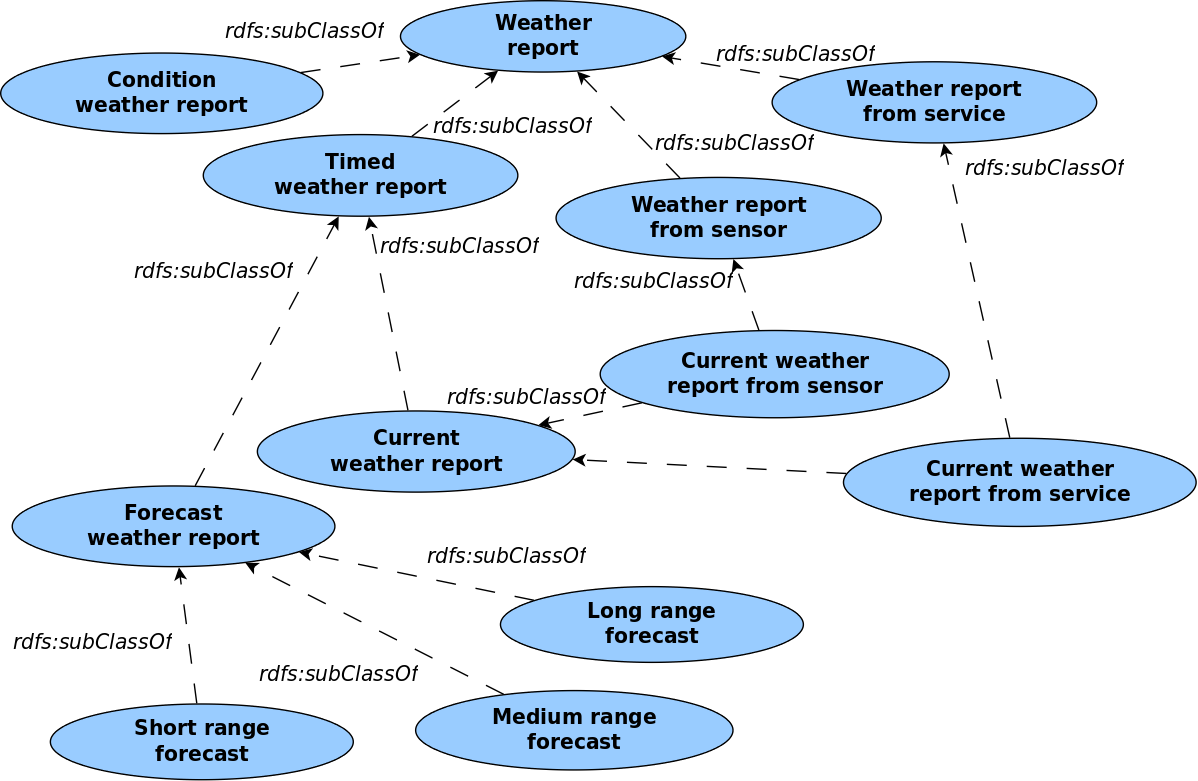
\includegraphics[width=\textwidth]{figures/diagrams/weather-report.pdf}
  \caption{Concept-classification tree for \Egls{weather report}}
  \label{fig:tree_weather_report}
\end{figure}

The concepts \Egls{short range weather report}, \Egls{medium range weather report} and \Egls{long range weather report} each do have sub-concepts which have been omitted from the above diagram for clarity. These sub-concepts are:
\begin{itemize}
  \item \Egls{short range weather report}: \emph{Forecast 1 hour weather report}, \emph{Forecast 2 hours weather report} and \emph{Forecast 3 hours weather report} for weather reports describing the weather in one, two and three hours, respectively.
  \item \Egls{medium range weather report}: \emph{Forecast 6 hour weather report} and \emph{Forecast 9 hours weather report} for weather reports describing the weather in 6 and 9 hours, respectively.
  \item \Egls{long range weather report}: \emph{Forecast 12 hour weather report}, \emph{Forecast 15 hours weather report}, \emph{Forecast 18 hours weather report}, \emph{Forecast 21 hours weather report} and \emph{Forecast 24 hours weather report} for weather reports describing the weather in 12, 15, 18, 21 and 24 hours, respectively.
\end{itemize}

A \Egls{weather source} can either be a \Egls{sensor source} or a \Egls{service source} (see figure~\ref{fig:tree_weather_source}).

\begin{figure}
  \centering
  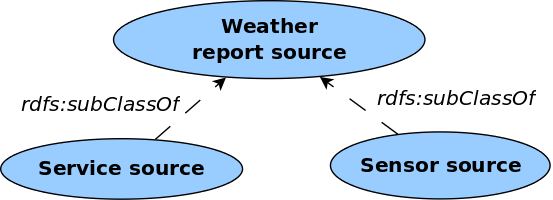
\includegraphics[width=.5\textwidth]{figures/diagrams/weather-report-source.pdf}
  \caption{Concept-classification tree for \Egls{weather source}}
  \label{fig:tree_weather_source}
\end{figure}

A \Egls{weather state} represents the set of weather phenomena that belong to a certain \Egls{weather report}. In order to emphasise certain combinations of instances of \Egls{weather phenomenon} being linked to the same instance of \Egls{weather state}, several sub-concepts of \Egls{weather state} are introduced (see section~\ref{sec:ontology_glossary}). The resulting tree is seen in figure~\ref{fig:tree_weather_state}.

\begin{figure}
  \centering
  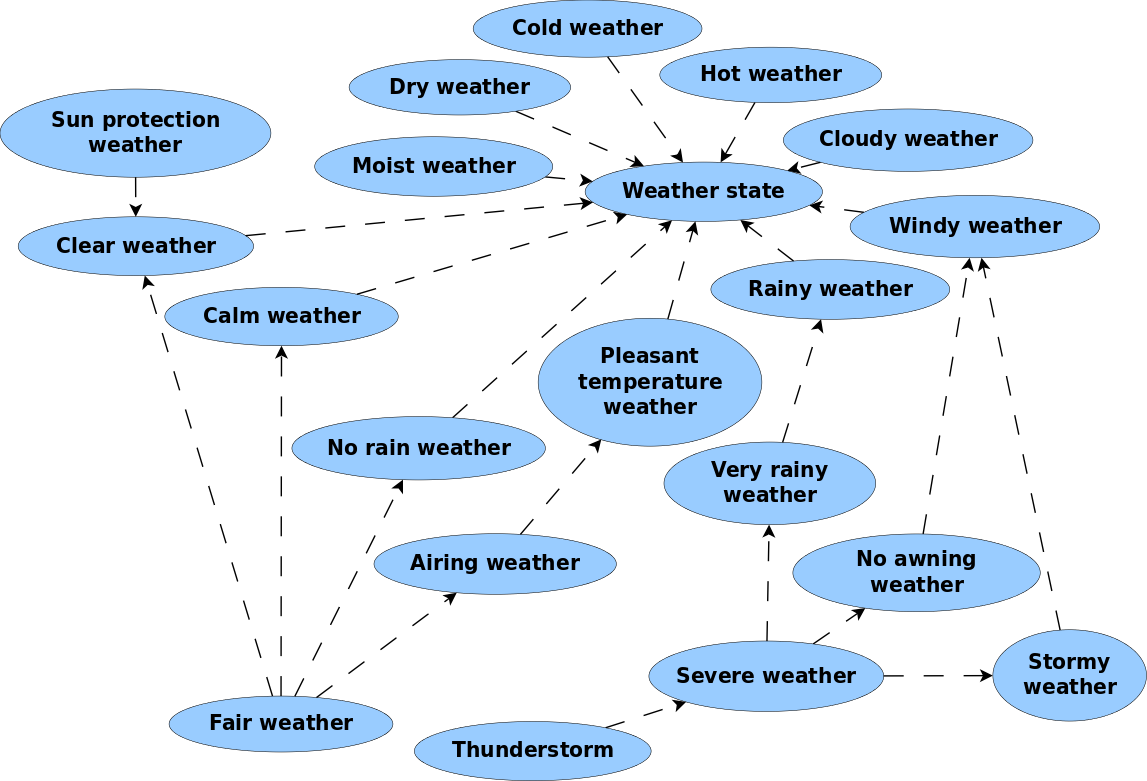
\includegraphics[width=\textwidth]{figures/diagrams/weather-state.pdf}
  \caption{Concept-classification tree for \Egls{weather state}. All properties are of type \emph{rdfs:subClassOf}}
  \label{fig:tree_weather_state}
\end{figure}

\subsection{Binary relations diagram}
\label{subsec:binary_relations_diagram}

The purpose of a \emph{Binary relations diagram} is to present all binary relations between concepts in the ontology (see figure~\ref{fig:binary_relations}).

\begin{figure}
  \centering
  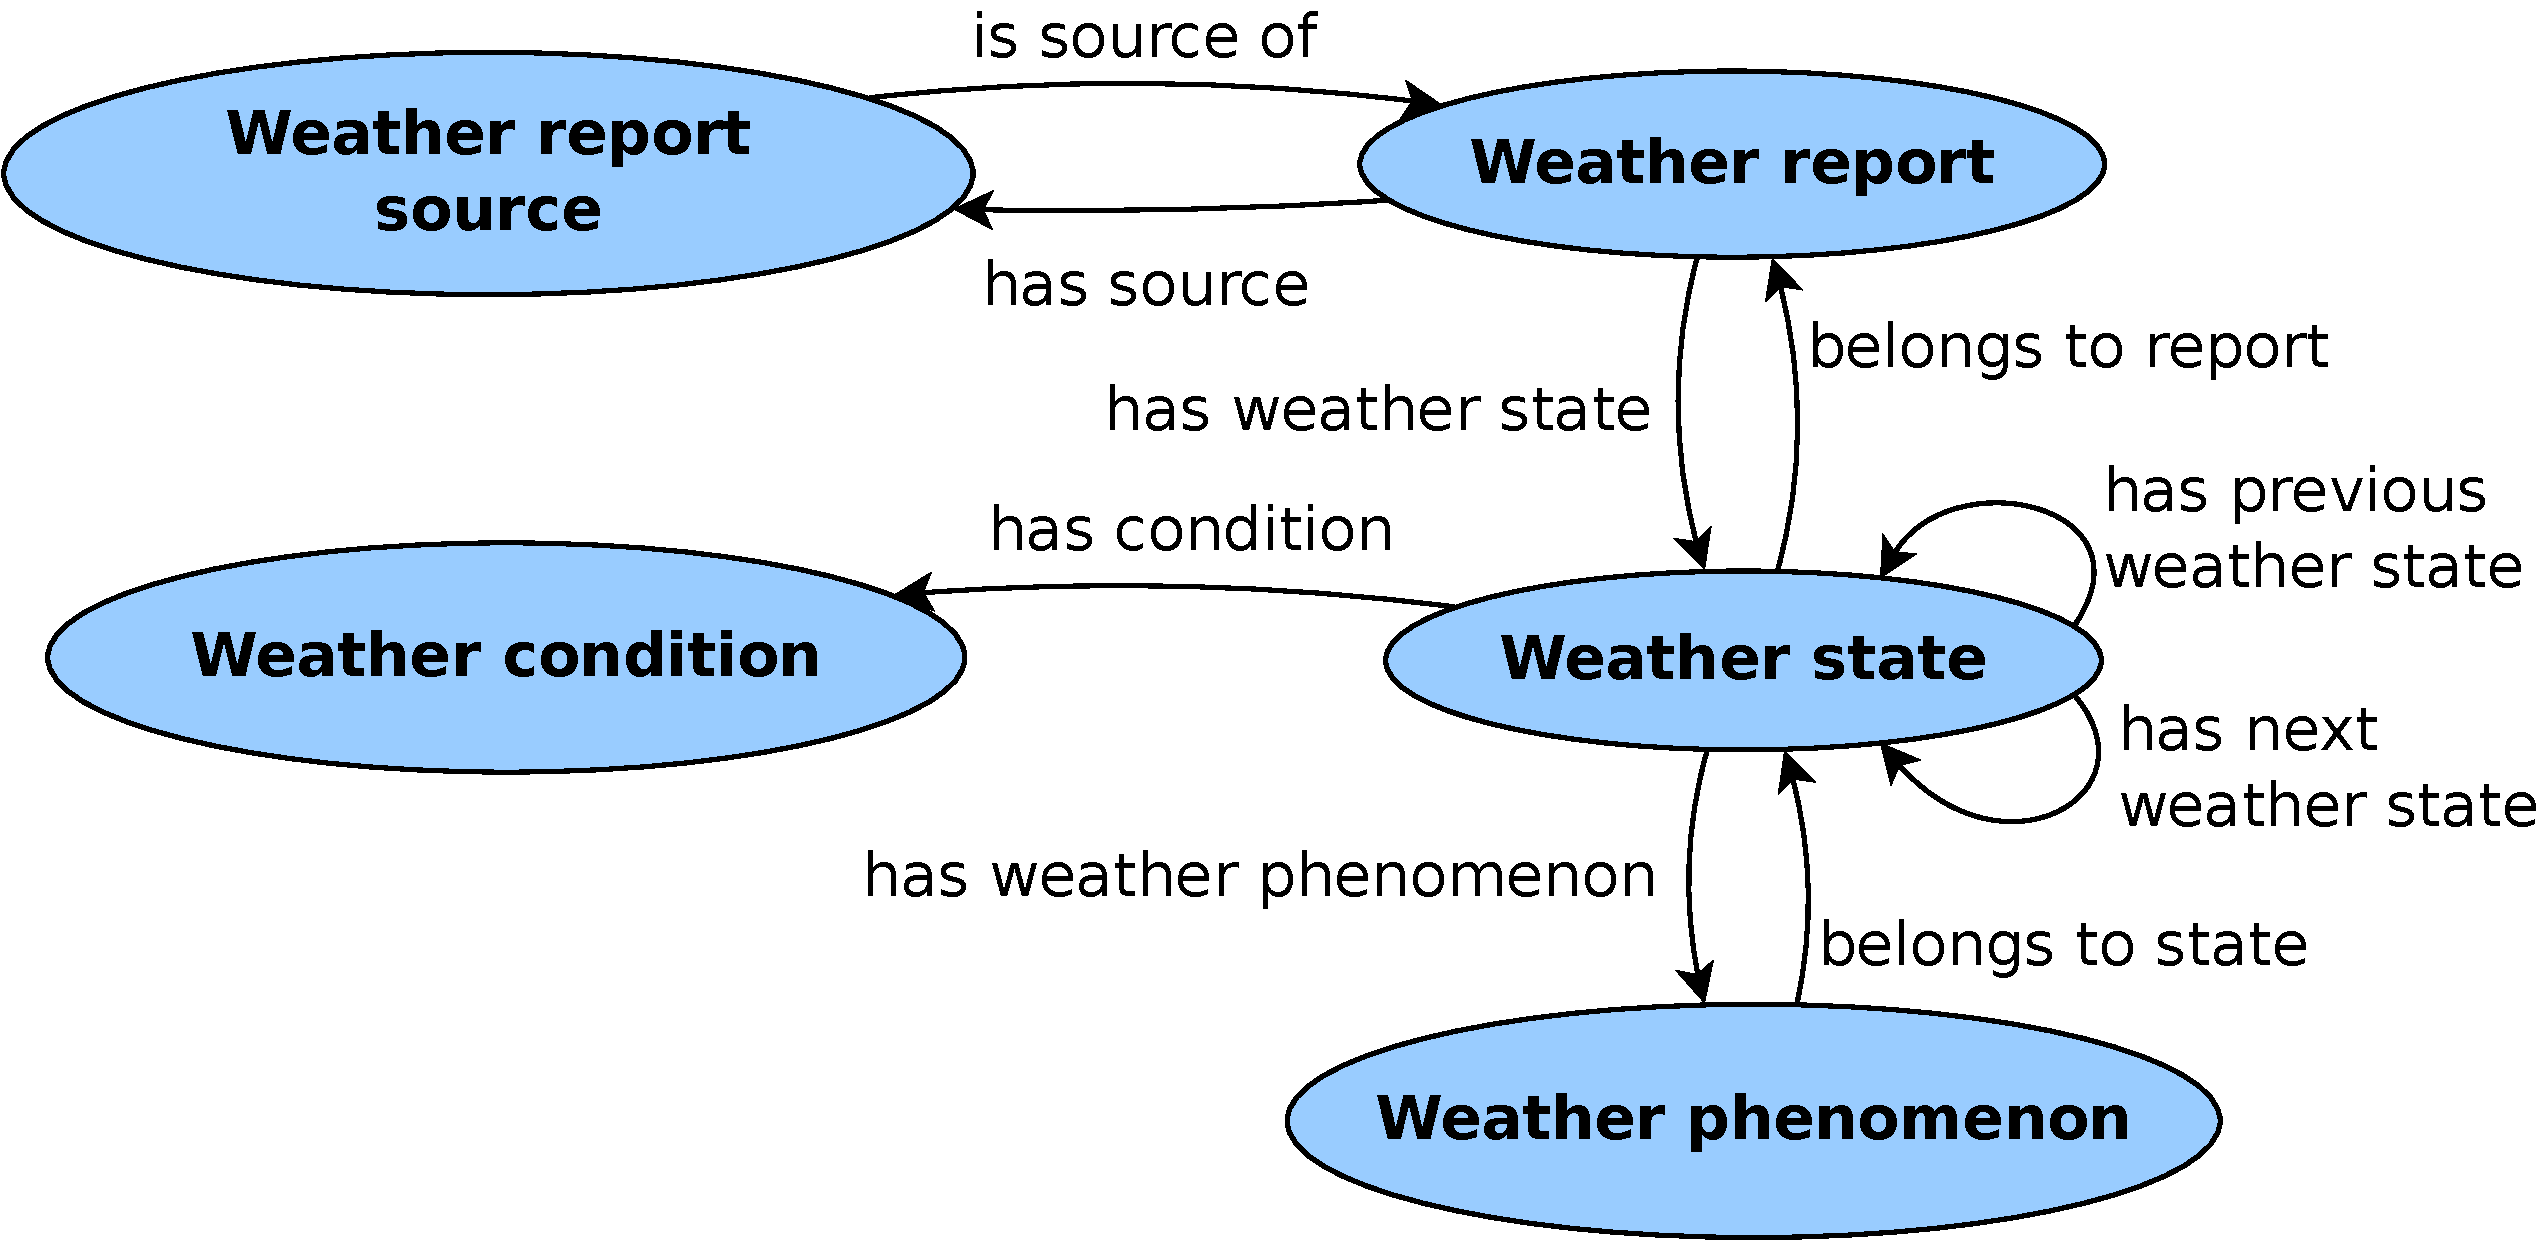
\includegraphics[width=.8\textwidth]{figures/diagrams/binary-relations.pdf}
  \caption{Binary relations diagram of \thinkhomeweather}
  \label{fig:binary_relations}
\end{figure}

\subsection{Concept dictionaries}
\label{subsec:concept_dictionaries}

A \emph{Concept dictionary} lists all concepts together with their names, instances, class attributes, instance attributes, and relations. For the sake of clarity, this table is split up into several tables, one for each of the concept-classification trees from section~\ref{sec:concept_classification_trees}.

The tables can be found in the appendix in figure~\ref{fig:concept_dict1} (\Egls{weather phenomenon}), figure~\ref{fig:concept_dict2} (\Egls{weather phenomenon}), figure~\ref{fig:concept_dict3} (\Egls{weather report}), figure~\ref{fig:concept_dict4} (\Egls{weather state}), and figure~\ref{fig:concept_dict5} (\Egls{weather source}). In these tables, sub-concepts having the same instances, class attributes, instance attributes and relations as their super-concepts are omitted. Furthermore, any columns that are not filled with any content in any row are omitted.

\subsection{Binary relations table}
\label{subsec:binary_relations_table}

The \emph{Binary relation table} specifies all relations from section~\ref{subsec:binary_relations_diagram} in detail. This includes the relations' names, their source and target concepts, their maximum source cardinalities, and their inverse relations, if any. The table can be found in the appendix in figure~\ref{fig:binary_relations_table}.

\subsection{Instance attributes table}
\label{subsec:instance_attributes_table}

An \emph{Instance attributes table} lists all instance attributes in \thinkhomeweather together with the concept where they belong to, their value type and value range, the unit of measurement and their cardinality. The \emph{Instance attributes table} can be found in the appendix in figure~\ref{fig:instance_attributes_table}.

The data types \emph{xsd:integer} and \emph{xsd:decimal} in the table refer to the types defined in \emph{XML Schema}\cite{xml-schema-datatypes}. For sake of simplicity, this table does not respect use the \emph{Measurements Unit Ontology} (\muo)\cite{MUO}. In the ontology, all attributes listed below that belong to a sub-concept of \Egls{weather phenomenon} do not refer to a literal as stated here. Instead, they link to a blank node of type \emph{Quality value} which in turn has two attributes, one for the literal value (named \emph{numerical value}) and one for the unit (named \emph{measured in}). The type given in the table below is the type of the value the property \emph{numerical value} refers to. See section~\ref{sec:ontology_imports} for details about the implementation of \muo in \thinkhomeweather.

\subsection{Class attributes table}
\label{subsec:class_attributes_table}

Many concepts within the \thinkhomeweather ontology define themselves to be specializations of other concepts. E.g. the concepts \Egls{very low pressure}, \Egls{low pressure}, \Egls{average pressure}, \Egls{high pressure} and \Egls{very high pressure} are all sub-concepts of \Egls{atmospheric pressure}. They all differ by the value of the instance attribute \egls{has pressure value} that every instance of \Egls{atmospheric pressure} has.

These concepts are summarized in the \emph{Class attributes table} in the appendix in figure~\ref{fig:class_attributes_table1}, figure~\ref{fig:class_attributes_table2}, and figure~\ref{fig:class_attributes_table3}. As in the \emph{Instance attributes tables} in section~\ref{subsec:instance_attributes_table}, this table does not respect the use of \muo; no units are specified.

\subsection{Instances table}
\label{subsec:instances_table}

The only pre-defined instances in \thinkhomeweather are the instances of the concept \Egls{weather condition}. Their details can be found in the \emph{Instance table} in the appendix in figure~\ref{fig:instances_table}.

\section{Integration}
\label{sec:integration}

One of the goals when designing an ontology is to reuse existing ontologies where possible\cite{reuse1,reuse2}. It the domain of \thinkhomeweather, four areas have been identified where existing ontologies can be reused: These are location data, measurement units, weather concepts and specifications of date and time. Chapter \ref{ch:existing_work} sheds some light on existing ontologies around the domain of weather data. In this section, the ontologies that have found to be eligible for reuse within \thinkhomeweather are presented.

\paragraph{Location data:}

Each \Egls{weather report} is valid for a certain location on Earth, given by \emph{latitude}, \emph{longitude} and \emph{altitude}. To handle such location data, the \emph{W3C Semantic Web Interest Group}\footnote{\href{http://www.w3.org/2001/sw/interest/}{http://www.w3.org/2001/sw/interest/}} developed the \emph{Basic Geo (WGS84 lat/long) Vocabulary}\cite{wgs84_vocabulary}. It introduces a concept called \emph{Spatial thing} and its attributes \egls{lat}, \egls{long} and \egls{alt} according to the \emph{WGS-84 geodetic reference system}\cite{WGS84}.

However, the vocabulary contains some data properties that are incorrectly defined to be annotation properties. Thus, they must be redefined to be data properties whenever used in an ontology.

\paragraph{Weather concepts:}

The \emph{SWEET} ontology\cite{SWEET}\footnote{\href{http://sweet.jpl.nasa.gov/ontology/}{http://sweet.jpl.nasa.gov/ontology/}} developed by the \emph{Jet Propulsion Laboratory} at the \emph{California Institute of Technology}\footnote{\href{http://www.jpl.nasa.gov/}{http://www.jpl.nasa.gov/}} offers a wide range of concepts, attributes and individuals for environmental and atmospherical phenomena, including all units that may be used in weather data ontologies. \emph{SWEET} is designed in a highly modular manner; there is a single \emph{OWL} file that provides definitions of measurement units. However, any file that is part of \emph{SWEET} depends on a number of other files belonging to that ontology and these in turn have dependencies. Thus, importing one of \emph{SWEET}'s \emph{OWL} files entails the import of a large number of other files; a simple ontology like \thinkhomeweather becomes hard to handle. Hence, reusing \emph{SWEET} is not an option.

Besides \emph{SWEET}, there is no ontology providing weather concepts that has been determined to be appropriate for use in the \thinkhomeweather ontology. Hence, \thinkhomeweather defines its own weather concepts.

\paragraph{Units of measurement:}

All instances of \Egls{weather phenomenon} have one or more attributes specifying details about the weather element that is being represented (refer to appendix~\ref{subsec:appendix_instance_attributes_tables} for details about these attributes). Each of these attributes assigns a numerical value to the \Egls{weather phenomenon}. To avoid confusion by the use of different units for one attribute (e.g. \si{\degree F} and \si{\celsius} for the \emph{temperature value}) the unit being used shall be added to the attribute value.

As the use of units of measurement is a topic that occurs in many ontologies, there are several different approaches to cope with it.

The \emph{Measurement Units Ontology}\footnote{\href{http://idi.fundacionctic.org/muo/muo-vocab.html}{http://idi.fundacionctic.org/muo/muo-vocab.html}}\cite{MUO} is a simple and light-weight approach to enrich measurement values in an ontology with appropriate units. Some of the most important units are pre-defined, others can easily be added when needed. The \emph{Measurement Units Ontology} (\muo) is still work in progress, however it is not expected that it might change heavily in the future. Everything that will be reused by other ontologies will remain unchanged. Hence, \muo can be imported into any ontology without problems.

Besides the \emph{Measurement Units Ontology}, several other ontologies have been examined, but all of them have shortcomings that render their use in the \thinkhomeweather ontology impossible. These ontologies are:
\begin{itemize}
  \item \textbf{\emph{SWEET}}: Besides concepts, attributes and individuals for atmospherical phenomena, \emph{SWEET} also comes with support for literals more precisely specified by units. However, as mentioned above, \emph{SWEET} is an ontology that is inappropriate for use in \thinkhomeweather.
  
  \item \textbf{\emph{QUDT}}: \emph{QUDT}\footnote{\href{http://www.qudt.org/}{http://www.qudt.org/}}, a set of ontologies for \emph{Quantities, Units, Dimensions and Data Types in OWL and XML}, is a promising approach for adding support for units to an \emph{OWL} ontology. However, \emph{QUDT} does not work in \protege together with the \emph{Pellet} reasoner. Using \emph{QUDT} would require several changes to its \emph{OWL} files. Hence, it cannot be used in the \thinkhomeweather ontology.
  
  \item \textbf{\emph{QUOMOS}}: The \emph{OASIS Quantities and Units of Measure Ontology Standard} (\emph{QUOMOS})\footnote{\href{https://www.oasis-open.org/committees/tc\_home.php?wg\_abbrev=quomos}{https://www.oasis-open.org/committees/tc\_home.php?wg\_abbrev=quomos}} is a project that aims at developing ``an ontology for quantities, systems of measurement units, and base dimensions for use across multiple industries''. However, as no deliverables have been released at the time of writing, it cannot be used in \thinkhomeweather.
  
  \item \textbf{OBO Foundry Initiative}: The \emph{OBO Foundry Initiative}\footnote{\href{http://obofoundry.org/}{http://obofoundry.org/}} is an initiative that aims at collecting ontologies for use in the biomedical domain. The list of \emph{The Open Biological and Biomedical Ontologies} (abbreviated by \emph{OBO}) includes an ontology for units of measurements\footnote{\href{http://obofoundry.org/cgi-bin/detail.cgi?id=unit}{http://obofoundry.org/cgi-bin/detail.cgi?id=unit}}\footnote{\href{http://code.google.com/p/unit-ontology/}{http://code.google.com/p/unit-ontology/}}. This ontology apparently covers most of the units that are used in the \thinkhomeweather ontology. However, it lacks any documentation and hence cannot be used in \thinkhomeweather.
  
  \item \textbf{OM}: The \emph{Ontology of Units of Measure and Related Concepts} (\emph{OM})\footnote{\href{http://www.wurvoc.org/vocabularies/om-1.6/}{http://www.wurvoc.org/vocabularies/om-1.6/}}\cite{OM} is another promising approach for adding measurement units to \emph{OWL} that even provides features like the conversion between different units for the same quantities and representation and checking of formulas. It is a rather large ontology (nearly \SI{2.4}{\mebi\byte} in \emph{RDF/XML syntax}) compared to the \thinkhomeweather ontology and related to the purpose it would fulfil in \thinkhomeweather; furthermore, at the time when the article about OM was published, development of \thinkhomeweather had already completed. Hence, \emph{OM} was not taken into account for being used in the \thinkhomeweather ontology.
\end{itemize}

Although the \emph{Measurement Units Ontology} does come with a few shortcomings (see section~\ref{sec:implementation}), it is the ontology that has been identified to be the the one that fits \thinkhomeweather requirements best.

\paragraph{Date and time:}

The attributes \egls{has start time}, \egls{has end time} and \egls{has observation time} of the concept \Egls{weather state} need to encode date and time information in an appropriate way.

For specifying temporal properties, the \emph{World Wide Web consortium} (\emph{W3C})\footnote{\href{http://www.w3.org/}{http://www.w3.org/}} offers a \emph{working draft}\cite{w3c-process} of \emph{OWL-Time}\cite{owl-time}, a \emph{Time Ontology in OWL}. It defines the concept called \Egls{temporal entity} that can either be an \Egls{instant} or an \Egls{interval}. Using appropriate attributes, the properties of a \Egls{temporal entity} are specified. Although \emph{OWL-Time} is in the state of a \emph{working draft} since September 2006, the main concepts and attributes that will be reused by other ontologies are likely to remain unchanged in future releases of that ontology.

\vspace{1em}

Section \ref{sec:implementation} describes the reuse of the aforementioned ontologies within the \thinkhomeweather ontology in detail.

\section{Implementation}
\label{sec:implementation}

After exhaustive analysis and structuring in the previous sections, the step of implementing the ontology has become a straight-forward task.

The \thinkhomeweather ontology is implemented in OWL using \protege 4.1 together with the \emph{Pellet} \emph{OWL} 2 Reasoner. \emph{Pellet} includes \emph{Pellint}\footnote{\href{http://weblog.clarkparsia.com/2008/07/02/pellint-an-ontology-repair-tool/}{http://weblog.clarkparsia.com/2008/07/02/pellint-an-ontology-repair-tool/}}, an ontology performance tool that uses a set of patterns to find possible performance problems in an \emph{OWL} ontology. \emph{Pellint} has been used intensively to ensure it does not report any problems that could affect reasoning performance.

To ensure that the reasoning of all sub-concepts of \egls{weather phenomenon}, \egls{weather state} and \egls{weather report} works correctly, \emph{JUnit}\footnote{\href{http://junit.org/}{http://junit.org/}} is used (see section~\ref{sec:importer_tests}). Every test case loads the \thinkhomeweather ontology using the \emph{Jena framework}, adds appropriate individuals and checks using the \emph{Pellet reasoner} if reasoning is performed in the desired manner.

During implementation of \thinkhomeweather in \emph{OWL}, the identifiers of concepts, properties and instances in this document are modified by removing all space characters and concatenating all parts of the identifier using \emph{camel case}\cite{CamelCase}, e.g. \Egls{weather state} becomes \emph{WeatherState} and \egls{has start time} becomes \emph{hasStartTime}. Hence, in the \emph{OWL} implementation, all identifiers match the regular expression \texttt{\textasciicircum[A-za-z0-9]+\$}.


\subsection{Imported ontologies}
\label{sec:ontology_imports}

During the implementation step, the ontologies listed in section \ref{sec:integration} need to be imported and integrated. Their use necessitates the application of certain patterns required by these ontologies.

\vspace{1em}

\emph{OWL-Time}\cite{owl-time} defines the concept \Egls{temporal entity} and its sub-concepts \Egls{instant} and \Egls{interval}, both having a self-explanatory name. The properties \egls{has start time}, \egls{has end time} and \egls{has observation time} of \egls{weather report} link to instants; however, only \egls{has observation time} is implemented to link an instance of \Egls{instant} to a \Egls{weather report}. For \egls{has start time} and \egls{has end time}, instances of \Egls{interval} are used. Such an instance represents the interval between the \egls{observation time} and the time the \Egls{weather report} is valid from/until (in hours). This simplifies reasoning of the sub-concepts of \Egls{weather report} which depend on the report's \egls{start time}; e.g. an instance of \emph{Forecast 1 hour weather report} can be defined as an instance of \Egls{weather report} having a \egls{start time} of \num{1} (hours).

Figure~\ref{fig:owl_time1} shows a \Egls{weather report} together with its with \egls{start time} and \egls{end time}; figure~\ref{fig:owl_time2} displays a \Egls{weather report} together with its \egls{observation time}. The \emph{Time Zone Ontology} that comes with \emph{OWL-Time} is not used by \thinkhomeweather. All times are given in \emph{UTC}.

\begin{figure}
  \centering
  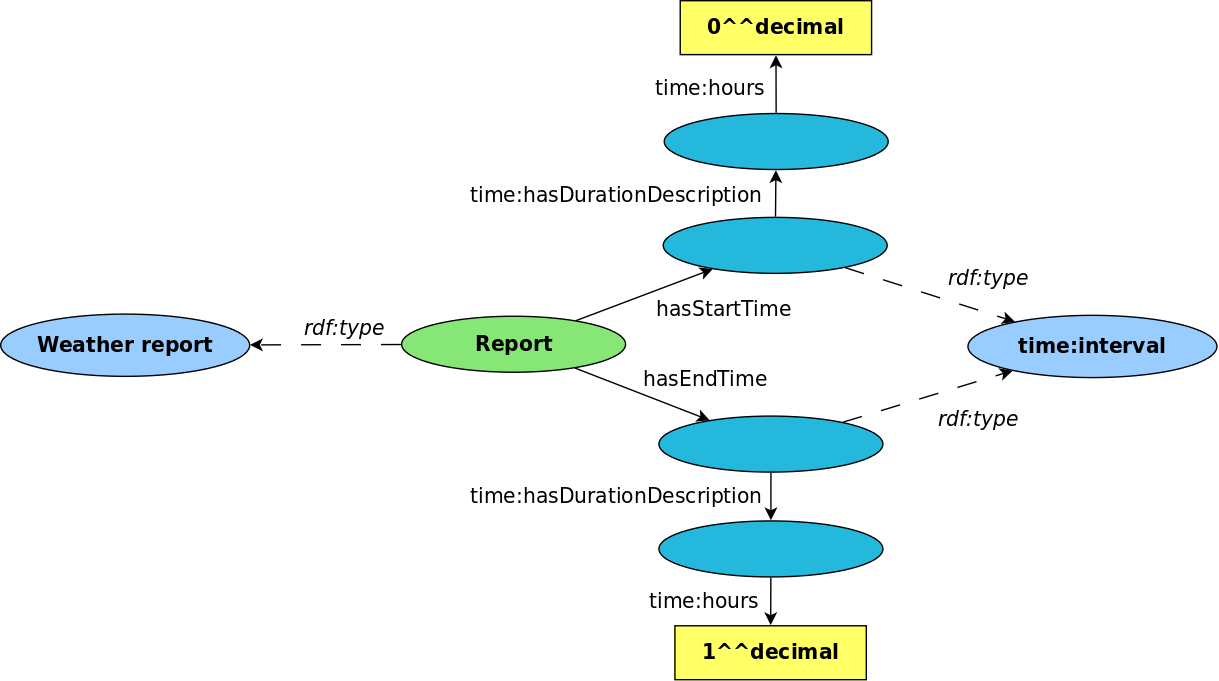
\includegraphics[width=\textwidth]{figures/diagrams/owl-time1.pdf}
  \caption{An instance of \Egls{current weather report} together with \egls{start time} and \egls{end time}}
  \label{fig:owl_time1}
\end{figure}

\begin{figure}
  \centering
  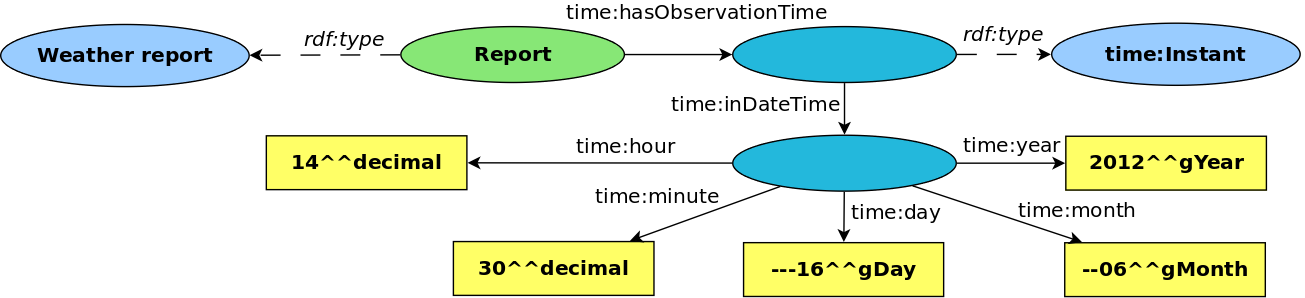
\includegraphics[width=\textwidth]{figures/diagrams/owl-time2.pdf}
  \caption{An instance of \Egls{weather report} together with its \egls{observation time} (\texttt{2012-06-16~14:30})}
  \label{fig:owl_time2}
\end{figure}

\vspace{1em}

Figure~\ref{fig:muo1} shows how an instance of \Egls{temperature} would be implemented if no ontology for units of measurements would be used. With the introduction of the \emph{Measurement Units Ontology} (\muo), the data property and the literal are removed; an object property that is a sub-property of \emph{Quality value} (which is defined by \muo) takes the place of the data property. It links to a blank node which in turn has two properties: \emph{Measured in} and \emph{numericalValue}. The property \emph{Measured in} is an object property that refers to the unit being used which is represented by an instance of \muo's concept \emph{Unit of measurement}. Using the data property \emph{numericalValue}, the literal is connected to the blank node. The resulting pattern is seen in figure~\ref{fig:muo2}.

\begin{figure}
  \centering
  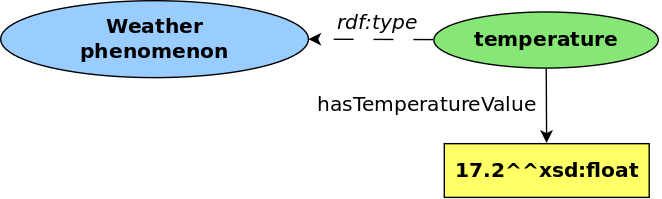
\includegraphics[width=.5\textwidth]{figures/diagrams/muo1.pdf}
  \caption{An instance of \Egls{temperature} together with the property \egls{has temperature value} representing a temperature of \SI{17.2}{\celsius} (without using a unit ontology)}
  \label{fig:muo1}
\end{figure}

\begin{figure}
  \centering
  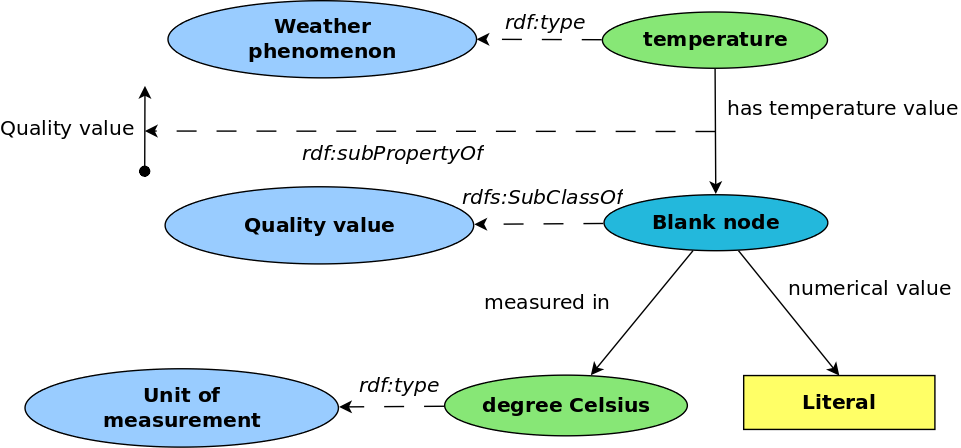
\includegraphics[width=.9\textwidth]{figures/diagrams/muo2.pdf}
  \caption{An instance of \Egls{temperature} together with the property \egls{has temperature value} representing a temperature of \SI{17.2}{\celsius} (using \muo)}
  \label{fig:muo2}
\end{figure}

\muo is an ontology that is easy to implement in an already-existing ontology. Its major drawback in the case of \thinkhomeweather is that it affects reasoning time negatively. Repeated tests showed that reasoning time increased by about $30 \%$ when introducing \muo. However, the slowdown caused by \muo is accepted in favour of the usage of units of measurement.

\vspace{1em}

Figure~\ref{fig:owl_wgs84} shows how the \egls{location} of a \Egls{weather report} is encoded.

\begin{figure}
  \centering
  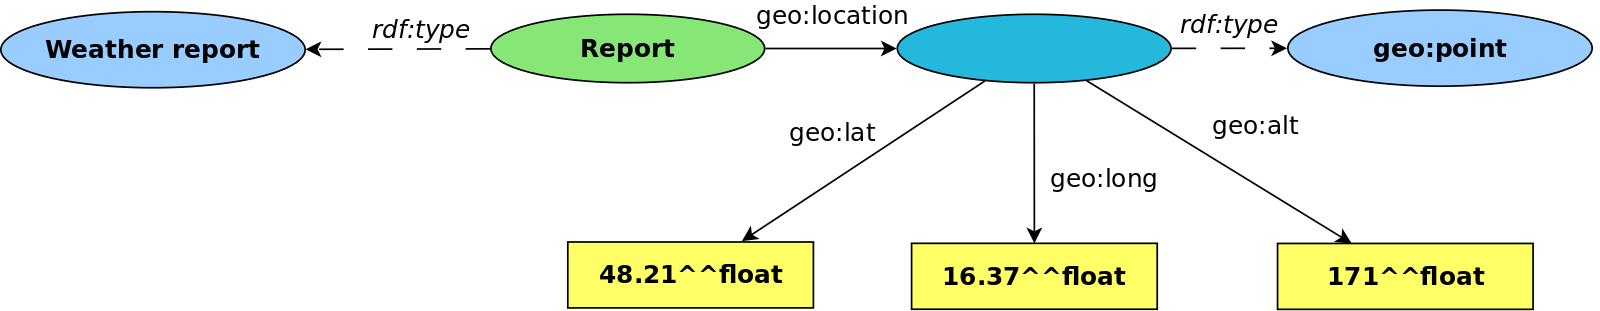
\includegraphics[width=\textwidth]{figures/diagrams/wgs84.pdf}
  \caption{An instance of \Egls{weather report} together with its \egls{location} (Vienna, Austria: N~\SI{48.21}{\degree}, E~\SI{16.37}{\degree}, \SI{171}{\metre} above \emph{MSL}).}
  \label{fig:owl_wgs84}
\end{figure}

\section{Evaluation}
\label{sec:ontology_evaluation}

After completing the implementation step, this section evaluates \thinkhomeweather regarding all non-functional requirements (section~\ref{sec:evaluation_non_functional}) and functional requirements (section~\ref{sec:evaluation_functional}) from section~\ref{sec:weather_information} and the \emph{Ontology Requirements Specification Document} in section~\ref{sec:ontology_specification}.

\subsection{Non-functional requirements}
\label{sec:evaluation_non_functional}

There are three non-functional requirements:

\begin{itemize}
  \item \textbf{Naming conventions}: All identifiers in \thinkhomeweather follow the naming conventions stated in section~\ref{sec:ontology_conventions}.
  \item \textbf{Documentation}: Due to following the \methontology approach, the ontology is well documented at every stage of development.
  \item \textbf{Usage of other ontologies}: \thinkhomeweather uses the \emph{Basic Geo (WGS84 lat/long) Vocabulary}, \muo and \emph{OWL-Time}; no ontology has been found that satisfies the requirements of \thinkhomeweather regarding concepts for weather data.
\end{itemize}

Thus, all non-functional requirements are met by \thinkhomeweather.

\subsection{Functional requirements}
\label{sec:evaluation_functional}

\thinkhomeweather meets its functional requirements if it provides answers to all competency questions. This section evaluates if answers are provided and how answers can be drawn from the ontology.

For the following questions, \thinkhomeweather can give straight answers:
\begin{itemize}
  \item What is the current weather situation?
  \item What will the weather situation be in one hour, in two hours, …, in 24 hours?
  \item What is the current temperature, humidity, wind speed, …?
  \item What will be the temperature, humidity, wind speed, … in one hour, in two hours, …, in 24 hours?
  \item Does it rain?
\end{itemize}
To answer any of these questions, the relevant instance of \Egls{weather report} must be identified. Via the property \egls{has weather state}, an instance of \Egls{weather state} is connected to it; this instance has in turn an arbitrary number of \egls{has weather phenomenon} properties each linking to an instance of \Egls{weather phenomenon}. The information from these instances of \Egls{weather phenomenon} provide the desired answer.

However, there are questions that cannot be answered by \thinkhomeweather as writing rules to infer answers would be too complicated in \emph{OWL}:
\begin{itemize}
  \item Will the weather change? Will the temperature, humidity, … rise or fall?
  \item Do we need to irrigate the garden?
\end{itemize}

Furthermore, there are questions that cannot be answered using an \emph{OWL} ontology due to the \emph{Open World Assumption} (\emph{OWA})\cite{open-world-assumption}. For instance, an \emph{OWL} reasoner cannot determine that some attribute value is the lowest one as it does not know whether there may be lower value it does not know anything about; the reasoner only knows about the presence of individuals and attribute values, but nothing about their absence.

\begin{itemize}
  \item What will be the minimum temperature, humidity, … over the next 24 hours? What about maximum values?
  \item Will it rain in the next hours? Will it rain today?
  \item Will there be sunshine today?
  \item Will there be severe weather?
  \item Will temperature drop/stay below \SI{0}{\celsius}?
  \item When can we open windows and when do we have to keep them shut?
  \item When do we need sun protection?
  \item When will it outside be colder than inside the house? When will it be warmer?
\end{itemize}

However, for each of the above competency questions, whether a direct answer can be given or not, \thinkhomeweather can provide all available data; an external program that does not rely on the \emph{Open World Assumption} can access this data and generate an answer.

Hence, the ontology constructed in this chapter complies with its specification in section \ref{sec:ontology_specification}.


% TODO acronyms
\chapter{The \emph{Weather Importer}}
\label{ch:weather_importer}

In previous chapters, two topics are discussed that are relevant for this chapter: Chapter~\ref{ch:weather_data} digs into the details of weather services that are available via Internet, with the example of the API by the \emph{Norwegian Meteorological Institute} (\yrno) that is found to best fit the requirements found at the \smarthomeweather project. Chapter~\ref{ch:smarthomeweather_ontology} describes the design of the \smarthomeweather ontology. Eventually, the ontology needs to be populated with data, i.e. individuals that comprise the current and future state of the weather at the desired location.

For that process, a standalone Java application has been developed. As its main purpose is to import weather data, it was named \emph{Weather Importer}.

At its current state of development, \emph{Weather Importer} obtains data only from \yrno in order to provide a reference implementation being both simple and functional, but it is designed to allow simple integration of other weather services that are available via Internet as well as data from local weather sensors.

The classes are arranged in two packages, \texttt{model} and \texttt{main}. The \texttt{model} package contains an object-oriented data model for the weather data being processed (see section~\ref{sec:importer_model}). All other classes belong to the \texttt{main} package, including the \texttt{Main} class providing the \texttt{main} method, the classes \texttt{TurtleStatement} and \texttt{TurtleStore} for output in \emph{Turtle syntax}\cite{Turtle} (see section~\ref{subsec:importer_turtle}), the interface \texttt{Importer}, and its reference implementation \texttt{YrNoImporter} (see section~\ref{subsec:importer_fetch}), \texttt{WeatherImporterProperties} which encapsulates the \emph{properties file} (see section~\ref{sec:importer_application}), and \texttt{WeatherImporterException}, an exception class that is used throughout the application.

All classes belonging to \emph{Weather Importer} include comments suitable for use with the \emph{Javadoc Tool}~\cite{javadoc}.

\section{The data model}
\label{sec:importer_model}

The core of \emph{Weather Importer} is formed by an object-oriented data model that can be found in the \texttt{model} package. This package contains classes that are to be instantiated in order to encapsulate all data that is collected from weather sensors and services. After processing the data in a manner that makes it suitable for use within the \smarthomeweather ontology, individuals and statements are generated and added to the ontology.

\begin{figure}
\centering
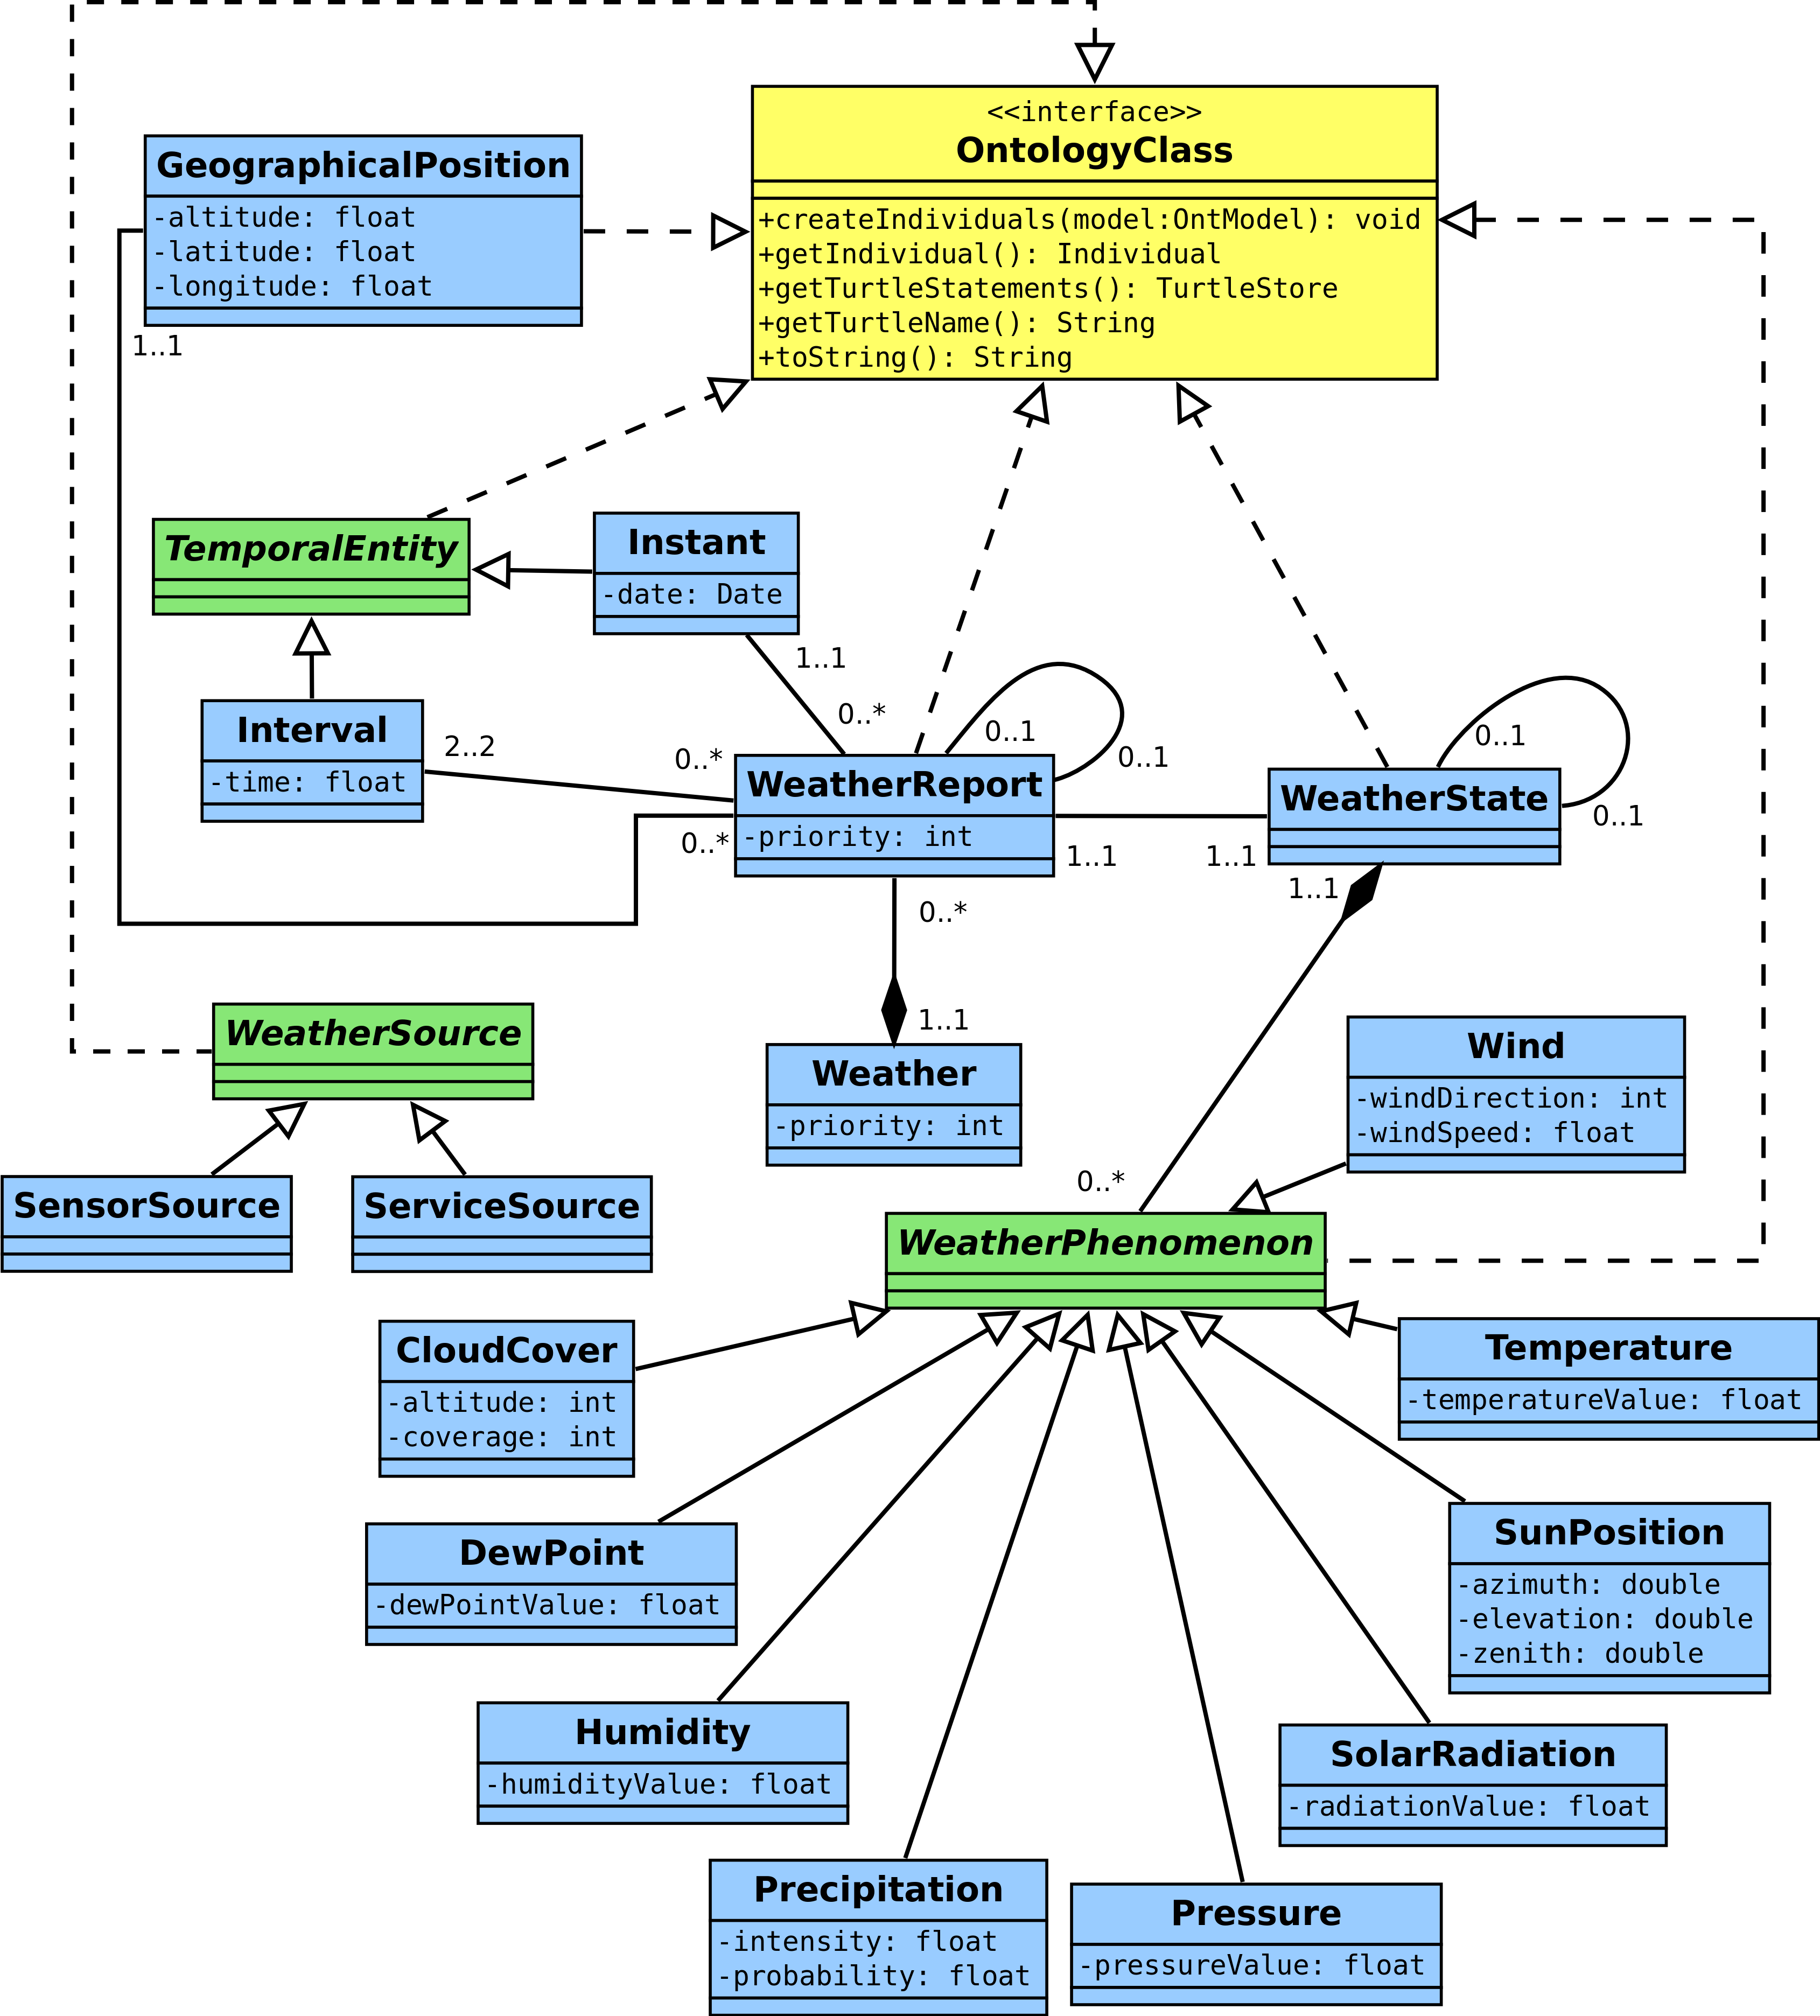
\includegraphics[width=\textwidth]{figures/diagrams/importer-model.pdf}
\caption{The domain model used in \emph{Weather importer}. See figure~\ref{fig:importer_model2} for a simplified diagram that shows only the most important classes.}
\label{fig:importer_model1}
\end{figure}

\begin{figure}
\centering
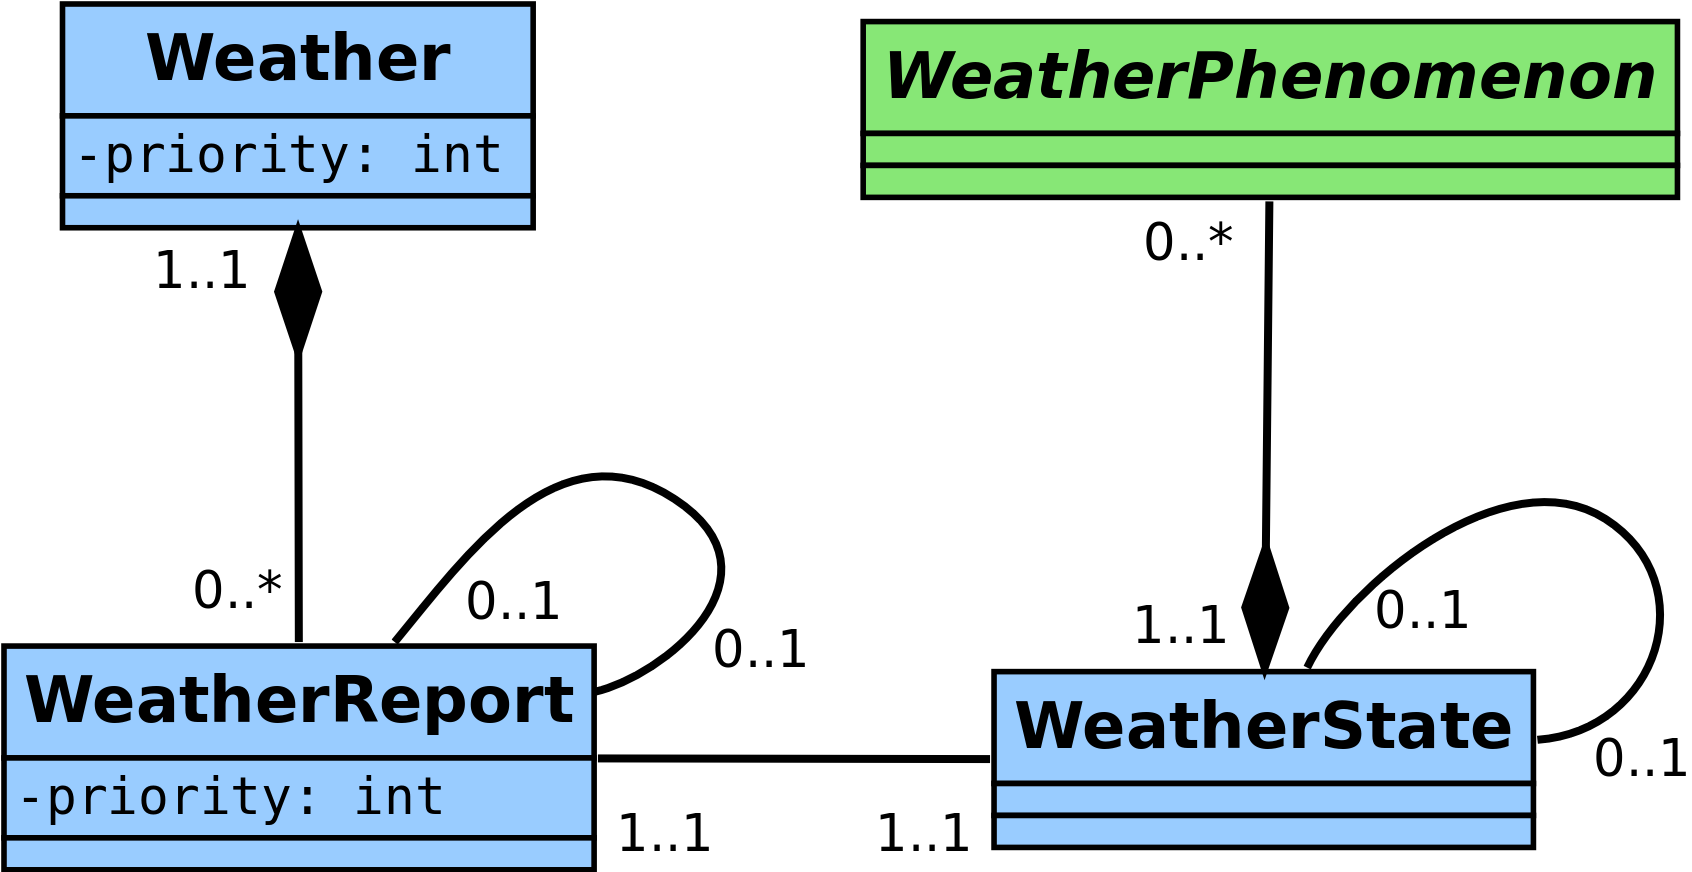
\includegraphics[width=.5\textwidth]{figures/diagrams/importer-model-simple.pdf}
\caption{The most important classes of the domain model used in \emph{Weather importer}. Refer to figure~\ref{fig:importer_model1} for a diagram showing all classes.}
\label{fig:importer_model2}
\end{figure}

The domain model in the package \texttt{model} which resembles the structure of the \smarthomeweather ontology is depicted in the \emph{UML} class diagram in figure~\ref{fig:importer_model1}; to give an overview, figure~\ref{fig:importer_model2} shows a simplified class diagram that shows only the most important classes \texttt{Weather}, \texttt{WeatherReport}, \texttt{WeatherState}, and \texttt{WeatherPhenomenon}.

Other than its name suggests, \texttt{OntologyClass} is an interface that is implemented by every class that corresponds to a concept (class) in the ontology. That interface defines a set of methods which are necessary to export an object's data either to individuals and statements for adding them to the ontology using \emph{Apache Jena}~\cite{apache_jena} or to a representation of the individuals and statements in \emph{Turtle syntax} (see section~\ref{sec:importer_application} below). The methods defined by \texttt{OntologyClass} are:
\begin{itemize}
  \item \texttt{createIndividuals()} creates individuals and statements holding the data that is stored in the object and adds them to the ontology. The method calls \texttt{createIndividuals()} for any objects that are connected to this object, with the exception of instances of \texttt{WeatherState} and \texttt{WeatherReport} that are linked together via the properties \texttt{previousState} and \texttt{previousReport}, respectively.
  
  \item \texttt{getIndividual()} returns the \texttt{Individual} object previously created by the method \texttt{createIndividuals()} that represents the main ontology individual described by the object. In some classes, due to the structure of the \smarthomeweather ontology and the ontologies being imported, calling \texttt{createIndividuals()} will add more than one individual to the ontology, e.g. an \texttt{Instant} creates an individual of type \Egls{instant} and one of type \emph{DateTimeDescription}\footnote{\emph{DateTimeDescription} is defined by \emph{OWL-Time} as the concept that represents the timestamp of an \Egls{instant}; the property \emph{inDateTime} links an instance of \emph{DateTimeDescription} to an instance of \Egls{instant}.}. \texttt{getIndividual()} will return the \texttt{Individual} object representing the \Egls{instant} individual; the corresponding \emph{DateTimeDescription} object can be obtained by querying the ontology for the statement having the previously returned
  \Egls{instant} individual as subject and the property \emph{inDateTime} as predicate.
  
  \item \texttt{getTurtleStatements()} returns an instance of \texttt{TurtleStore} that contains a set of \texttt{TurtleStatement} objects each representing an RDF triple in \texttt{Turtle syntax}. The instance being returned contains all data that calling \texttt{createIndividuals()} would add to the ontology. See section~\ref{subsec:importer_turtle} for details.
  
  \item \texttt{getTurtleName()} returns the qualified name of the individual represented by the object that is used in in the \texttt{TurtleStatement}s returned by calling \texttt{getTurtleStatements()}. In case \texttt{createIndividuals()} creates more than one individual, the method only yields the name of the individual returned by \texttt{getIndividual()}.
  
  \item \texttt{toString()} returns a textual representation of the object (for debugging purposes).
\end{itemize}

The classes inside the package \texttt{model} are:
\begin{itemize}
  \item \texttt{GeographicalPosition} resembles the concept \Egls{point} of the \emph{Basic Geo (WGS84 lat/long) Vocabulary}\cite{wgs84_vocabulary} that is imported into the \smarthomeweather ontology.
  
  \item \texttt{TemporalEntity} corresponds to the concept \Egls{temporal entity} in the \emph{OWL-Time}\cite{owl-time} ontology. The are two sub-classes, \texttt{Instant} and \texttt{Interval} that resemble the concepts \Egls{instant} and \Egls{interval}, respectively.
  
  \item \texttt{WeatherPhenomenon} corresponds to the concept \Egls{weather phenomenon} in the \smarthomeweather ontology. As it is an abstract class, only its subclasses \texttt{CloudCover}, \texttt{DewPoint}, \texttt{Humidity}, \texttt{Precipitation}, \texttt{Pressure}, \texttt{SolarRadiation}, \texttt{SunPosition}, \texttt{Temperature} and \texttt{Wind} can be instantiated that each resemble the corresponding concept of the ontology.
  
  \item \texttt{WeatherReport} corresponds to the concept \Egls{weather report}.
  
  \item \texttt{WeatherSource} corresponds to the concept \Egls{weather source}. It is an abstract class and has two subclasses \texttt{SensorSource} and \texttt{ServiceSource} resembling the concepts \Egls{sensor source} and \Egls{service source}, respectively.
  
  \item \texttt{WeatherState} corresponds to the concept \Egls{weather state}.
  
  \item \texttt{Weather} has no counterpart in the ontology; it represents a collection of instances of \texttt{WeatherReport} which are obtained from sensors and/or services at the same time.
\end{itemize}

Additionally, there is an enumeration named \texttt{WeatherConditions} having values that each correspond to the individuals predefined by the ontology for the concept \Egls{weather condition}.

\section{The application}
\label{sec:importer_application}

The \emph{Weather Importer} application basically performs three tasks when being launched: It reads the \smarthomeweather ontology in \emph{RDF/XML syntax}\cite{RDF_XML} from a file, modifies it in some way and and writes the modified ontology into another file, either in \emph{RDF/XML syntax} or in \emph{Turtle syntax}\cite{Turtle}. There are four operation modes that are covered below: \texttt{fetch}, \texttt{timestamps}, \texttt{remove} and \texttt{turtle}.

The application depends on the \emph{Apache Jena} framework~\cite{apache_jena} (successfully tested with 2.10.0). For the unit tests (see section~\ref{sec:importer_tests}), \emph{JUnit}~\cite{junit} (4.11), the \emph{Pellet} \eacs{OWL} 2 reasoner~\cite{pellet} (2.3.0) and \emph{Cobertura}~\cite{cobertura} (1.9.4.1) are used. The version numbers given in parentheses give the versions of the most recent releases of the libraries at the time of writing. Newer releases may work, but have not been tested.

\emph{Weather Importer} comes with a build script for \emph{Apache Ant}~\cite{apache_ant} that provides target definitions for compiling, running and testing the application:

\begin{itemize}
  \item The targets \texttt{compile} and \texttt{compile\_test} compile the application and the \emph{JUnit} test cases, respectively. \texttt{dist} generates two \emph{JAR} files~\cite{jar}, one containing the application and one for the class that imports weather data from \yrno. \texttt{clean} removes all files and directories generated by the aforementioned targets and the target \texttt{javadoc}; \texttt{rebuild} executes \texttt{clean}, \texttt{compile}, \texttt{dist} and \texttt{compile\_test} consecutively.
  \item The targets \texttt{fetch}, \texttt{timestamps}, \texttt{remove} and \texttt{turtle} launch the application in the respective modes.
  \item The target \texttt{test} runs the \emph{JUnit} test cases; \texttt{coverage} generates a coverage report using \emph{Cobertura}, i.e. an overview about which parts of the application's code are covered by the test cases (see section~\ref{sec:importer_tests} for details).
  \item The target \texttt{javadoc} generates documentation from comments in the source code using the \emph{Javadoc Tool}~\cite{javadoc}.
\end{itemize}

Various parameters of \emph{Weather Importer} are configurable using a \emph{properties file}~\cite{java_properties} which provides the location for which weather data shall be fetched (given by latitude, longitude and altitude), the timestamps relative to the current time in hours for which instances of \texttt{WeatherReport} shall be created, names of input and output files and the name of the class that fetches weather data. Additional options required by an implementation of the \texttt{Importer} interface may be added.

\subsection{\texttt{fetch} mode}
\label{subsec:importer_fetch}

In \texttt{fetch} mode, \emph{Weather Importer} reads the \smarthomeweather ontology in \emph{RDF/XML syntax} from a file using the \emph{Apache Jena} framework and fetches weather data for the desired location from a weather service via Internet.

To provide the reference implementation that is found in the class \texttt{YrNoImporter}, \emph{Weather Importer} obtains weather data from \yrno as described in section~\ref{sec:weather_data_yr_no}. Any other sources for weather data, regardless whether that sources are weather sensors, Internet weather services or any combination of a set of these, can be utilized by creating a class that implements the interface \texttt{Importer}. This interface defines a single method named \texttt{fetchWeather()} that returns a \texttt{Weather} object containing all weather data obtained from sensors and/or services.

By calling the method \texttt{createIndividuals()} of that \texttt{Weather} object, the weather data is added \emph{Apache Jena}'s in-memory representation of the ontology. Eventually, the modified ontology is written back to a file in \emph{RDF/XML} syntax.

As most weather services do not provide data for arbitrary points of time, the \texttt{Weather} class provides the method \texttt{normalizeWeatherReports()}. It transforms the data encapsulated by the \texttt{Weather} object in the following ways:
\begin{itemize}
  \item Each associated \texttt{WeatherReport} object that covers a period of more than one hour is replaced by several \texttt{WeatherReport} objects, one for each hour. All associated instances of \texttt{WeatherReport} and \texttt{WeatherPhenomenon} are cloned appropriately.
  
  \item If there is more than one \texttt{WeatherReport} object covering the same period of time, all data from these objects are merged into one object; the remaining objects will be discarded.
  
  \item In case there is no data for a period of time, it is calculated using linear interpolation from data before and after the missing period\cite{maths}.
  
  \item An instance of \texttt{SunPosition} is associated to each instance of \texttt{WeatherState}. The sun position data is calculated using the \emph{PSA algorithm}\cite{PSA_algorithm} (refer to section~\ref{sec:sun_position} for details); the C++ reference implementation of the \emph{PSA algorithm}~\cite{psa_online} was ported to Java.
\end{itemize}

Additionally, the class \texttt{WeatherState} provides the method \texttt{mergePhenomena()} which merges all instances of \texttt{WeatherPhenomenon} of the same type that are associated to that instance of \texttt{WeatherState}. Actual merging of values takes place in the constructors of the subclasses of \texttt{WeatherPhenomenon}; all current implementations merge values by calculating the arithmetic mean of all values provided\cite{maths}.

Both methods provide the developer of an implementation of the interface \texttt{Importer} with more flexibility on how to import weather data: There is no need to create a separate instance of \texttt{WeatherReport} for every possible period of time; each \texttt{WeatherReport} object may cover more than one hour and more than one instance of each subclass of \texttt{WeatherPhenomenon} may be associated to each instance of \texttt{WeatherState}. The latter eases merging values from several sources (e.g. an Internet weather service and a set of weather sensors).

\subsection{\texttt{timestamps} mode}

% TODO reference to the description of this process in the chapter about the smarthomeweather ontology?
As discussed in section ?, there are two ways to update weather data in the \smarthomeweather ontology:
\begin{itemize}
  \item The data can be reobtained using the \texttt{fetch} mode into a copy of the ontology that does not contain any weather data. If it does contain any weather data, it can be removed using the \texttt{remove} mode (see below).
  \item Alternatively, the timestamps of all instances of the \Egls{weather report} concept in order to make them correspond to the current time.
\end{itemize}

The latter option is implemented in \emph{Weather Importer} as the \texttt{timestamps} mode. That mode is based on the timestamps of each \Egls{weather report} individual being specified by the difference to the current time in hours.

\begin{figure}
\begin{lstlisting}
weather:interval0.0         time:hasDurationDescription           weather:hour0.0 .
weather:interval1.0         time:hasDurationDescription           weather:hour1.0 .
weather:interval2.0         time:hasDurationDescription           weather:hour2.0 .
weather:interval3.0         time:hasDurationDescription           weather:hour3.0 .
weather:interval4.0         time:hasDurationDescription           weather:hour3.0 .

weather:weatherReport2      weather:hasStartTime                  weather:interval2.0 ;
                            weather:hasEndTime                    weather:interval3.0 .

weather:weatherReport3      weather:hasStartTime                  weather:interval3.0 ;
                            weather:hasEndTime                    weather:interval4.0 .

weather:weatherReport2      weather:hasObservationTime            weather:instant0 .
weather:weatherReport2      weather:hasObservationTime            weather:instant0 .

weather:instant0            time:inDateTime                       weather:dateTime0 .

weather:dateTime0           a                                     time:DateTimeDescription ;
                            time:unitType                         time:unitMinute ;
                            time:minute                           44 ;
                            time:hour                             12 ;
                            time:day                              "---02"^^xsd:gDay ;
                            time:month                            "--03"^^xsd:gMonth ;
                            time:year                             "2013"^^xsd:gYear .
\end{lstlisting}
\caption{Example statements generated by \emph{Weather Importer} running in \texttt{fetch} mode.}
\label{fig:importer_timestamps1}
\end{figure}

% TODO fix highlighting
\begin{figure}
\begin{lstlisting}[escapechar=!]
weather:interval0.0         time:hasDurationDescription           weather:hour0.0 .
weather:interval1.0         time:hasDurationDescription           weather:hour1.0 .
weather:interval2.0         time:hasDurationDescription           weather:hour2.0 .
weather:interval3.0         time:hasDurationDescription           weather:hour3.0 .
weather:interval4.0         time:hasDurationDescription           weather:hour3.0 .

@@weather:weatherReport2      weather:hasStartTime                  weather:interval0.0 ;@@
@@                            weather:hasEndTime                    weather:interval1.0 .@@

@@weather:weatherReport3      weather:hasStartTime                  weather:interval1.0 ;@@
@@                            weather:hasEndTime                    weather:interval2.0 .@@

weather:weatherReport2      weather:hasObservationTime            weather:instant0 .
weather:weatherReport2      weather:hasObservationTime            weather:instant0 .

weather:instant0            time:inDateTime                       weather:dateTime0 .

weather:dateTime0           a                                     time:DateTimeDescription ;
                            time:unitType                         time:unitMinute ;
@@                            time:minute                           58 ;                @@
@@                            time:hour                             14 ;                @@
                            time:day                              "---02"^^xsd:gDay ;
                            time:month                            "--03"^^xsd:gMonth ;
                            time:year                             "2013"^^xsd:gYear .
\end{lstlisting}
\caption{Example statements modified by \emph{Weather Importer} running in \texttt{timestamps} mode about two hours after the running it in \texttt{fetch} mode. See figure~\ref{fig:importer_timestamps1} for the statements generated in the initial run; statements modified in \texttt{timestamps} mode are highlighted.}
\label{fig:importer_timestamps2}
\end{figure}

In \texttt{timestamp} mode, for each \Egls{weather report} individual stored in the ontology its observation time is retrieved and the difference to the current time in hours is calculated. This difference is then subtracted from both the individual's start time and end time properties; the difference is added to the individual's observation time. Figure~\ref{fig:importer_timestamps1} shows a part of the statements generated by running \emph{Weather Importer} in \texttt{fetch} mode; figure~\ref{fig:importer_timestamps2} shows the statements that have been modified by \emph{Weather Importer} running in \texttt{timestamps} mode two hours later.

After \emph{Weather Importer} has finished, the \emph{OWL} reasoner must be run using the new data in order to update all knowledge that is produced by the reasoner. E.g., in the example shown in figures~\ref{fig:importer_timestamps1} and~\ref{fig:importer_timestamps2}, an instance of \Egls{weather report} that was previously reasoned to be an instance of the concept \emph{Forecast 2 hours weather report} becomes an instance of \Egls{current weather report}, an instance of \emph{Forecast 3 hours weather report} becomes an instance of \emph{Forecast 1 hours weather report} and so on.

\subsection{\texttt{remove} mode}

In \texttt{remove} mode, the \emph{Weather Importer} takes an ontology in \emph{RDF/XML syntax} from a file using \emph{Apache Jena}. All weather data is removed and the resulting ontology is written back to a file in \emph{RDF/XML syntax}. This file can then be used as input to \emph{Weather Importer}'s \texttt{fetch} mode.

\subsection{\texttt{turtle} mode}
\label{subsec:importer_turtle}

The \texttt{turtle} mode is a mode that was created for debugging reasons; in that mode \emph{Weather Importer} performs the same steps as in \texttt{fetch} mode, with the following differences:
\begin{itemize}
  \item The \smarthomeweather ontology is not read from a file. Hence, the output consists only of the statements generated from the weather data that is imported.
  \item The \emph{Apache Jena} framework is not used. This enables a developer to distinguish between an error in the usage of \emph{Apache Jena} or an error somewhere else.
  \item For better readability, \emph{Turtle syntax} is used for output instead of \emph{RDF/XML}.
\end{itemize}

The \texttt{turtle} mode is not necessary for productive use of \emph{Weather Importer}. However, it is kept for providing a demonstrative description of \emph{Weather Importer}'s output and for easing future debugging, if necessary.

\begin{figure}
\centering
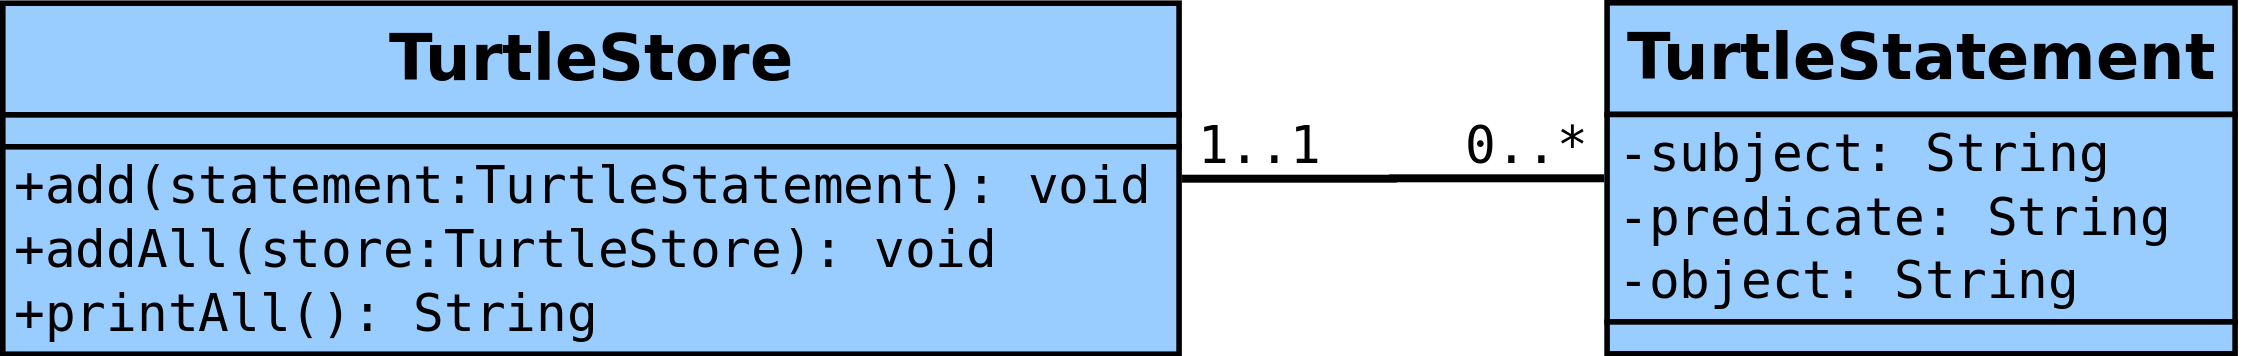
\includegraphics[width=.7\textwidth]{figures/diagrams/turtlestore.pdf}
\caption{Classes used for output in \emph{Turtle syntax}}
\label{fig:importer_turtlestore}
\end{figure}

Figure~\ref{fig:importer_turtlestore} shows the two classes \texttt{TurtleStatement} and \texttt{TurtleStore} that provide a data structure for output in \emph{Turtle syntax}. \texttt{TurtleStatement} represents a single \emph{RDF} statement in turtle syntax; \texttt{TurtleStore} encapsulates a set of \texttt{TurtleStatement} objects and provides a method for writing all statements to a file.

Section~\ref{sec:appendix_turtle_output} in the appendix shows a part of the output generated by \emph{Weather Importer} in \texttt{turtle} mode.

\section{Unit tests}
\label{sec:importer_tests}

\emph{Weather Importer} incorporates a set of \emph{JUnit}~\cite{junit} tests that covers reasoning in the \smarthomeweather ontology and the application itself. For testing correct reasoning, the \emph{Apache Jena} framework and the \emph{Pellet} reasoner are used.

The following test categories are implemented:
\begin{itemize}
  \item Tests for \emph{OWL} reasoning concerning single individuals of the ontology; e.g. an instance of \Egls{weather phenomenon} that has a \egls{has temperature value} property must be reasoned to be an instance of \egls{temperature}.
  \item Tests that involve reasoning for instances of several concepts; e.g. correct reasoning of \Egls{calm weather}.
  \item Tests for the import of weather data from \yrno.
  \item Tests for the output in \emph{Turtle syntax}.
\end{itemize}

% TODO mention untested parts
\begin{comment}
The following parts of the application are not covered by unit tests:

\begin{itemize}
  \item bla
  \item blubb
  \item foo
  \item bar
\end{itemize}
\end{comment}


\chapter{Conclusion}
\label{ch:conclusion}
% TODO unsourced?
% TODO uncomment
% \chapterquotation{If you want a happy ending, that depends, of course, on where you stop your story.}{Orson Welles}

% TODO extend: Ich finde die Conclusion gehört nochmals überarbeitet. Hierbei sollten nicht nur die Chapters sowie ihr Inhalt nochmals präsentiert werden, sondern vielmehr ein Resümee gezogen werden, was mit dieser Diplomarbeit erreicht wurde, sowie nochmals der "main outcome" in Kurzfassung beschrieben werden. Der Inhaltsüberblick über die einzelnen Chapter kann gerne drin bleiben, jedoch muss die Conclusion um die genannte Zusammenfassung erweitert werden.


\section{Summary}

This thesis a weather data model based on an \eacs{OWL} ontology, a Java application for importing data into that model, and all prerequisites leading to these two outcomes.

After Chapter~\ref{ch:intro} gives an introduction into the motivation behind the thesis and describes the problem statement, the intended goal and the methodological approach, Chapter~\ref{ch:existing_work} discusses the foundations the thesis builds upon: Ontologies, ontology related technologies like \eacs{RDF}, \eacs{RDFS}, or \eacs{OWL}, \thinkhome, already existing ontologies for weather data, and ontologies that cover information related to the domain covered by \smarthomeweather. Chapter~\ref{ch:weather_data} then focuses on weather data that is available from both locally installed weather sensors as well as from weather services accessible via Internet. This chapter then identifies a set of weather phenomena which \smarthomeweather shall cover and determines further details about the domain of weather data as used in the present context.
Of the weather services being discussed, \yrno is selected for providing a reference implementation for the import of weather data into \smarthomeweather in a later step. Chapter~\ref{ch:development_approaches} sheds light on five different approaches towards the development of new ontologies from scratch. The approaches are compared to each other and one of them, \methontology, is identified as the one that fits the requirements for designing \smarthomeweather best.

Eventually, Chapter~\ref{ch:smarthomeweather_ontology} applies \methontology to \smarthomeweather and describes every step in a detailed manner. As the data model itself does not contain any weather data, in Chapter~\ref{ch:weather_importer} the \emph{Weather Importer}, a Java application, is developed which accesses \yrno to retrieve weather data for a certain location, transforms the data being obtained and adds them to the data model of \smarthomeweather. Furthermore, the \emph{Weather Importer} includes a comprehensive set of \emph{JUnit} test cases which ensure that \smarthomeweather and the \emph{Weather Importer} work as expected.

\vspace{1em}

\section{Outlook}

% TODO interoperability with other sources of data
The current version of \smarthomeweather comes with a few shortcomings that require future work in order to resolve them. Not all of these problems lie in the scope of \smarthomeweather. The main problems arising are:

\begin{itemize}
  \item There are a few situations that expose bugs in \protege and the \emph{Pellet} reasoner. While it is possible to develop ontologies using these technologies which cover a certain domain, it is hardly avoidable to run into bugs that manifest themselves in the form of incomprehensible error messages. In that case, the ontology needs to be modified slightly to work around these bugs. Unfortunately, during the development of \smarthomeweather, it has not been possible to track these bugs down in order to find their reason and to fix them. Future work that resolves these bugs may ease the work with \protege, \emph{Pellet}, and \smarthomeweather.
  
  \item At the time of writing, \emph{OWL-Time}~\cite{owl-time} (see Section~\ref{subsec:date_ontologies}) has not reached the state of being a \emph{\eacs{W3C} recommendation}~\cite{w3c-process}; since it was first published more than six years ago, it is a \emph{working draft}. Although it can be assumed that the core concepts and relations defined by \emph{OWL-Time} will not change regarding their syntax and semantics, using technologies that are not yet published as being in a stable state always leaves a stale taste. % TODO rephrase "to leave a stale taste"
  
  \item Similar problems arise from the use of the \emph{Basic Geo (\eacs{WGS84} lat/long) Vocabulary}~\cite{wgs84_vocabulary}. This technology has not even been submitted to the \emph{\eacs{W3C} recommendation track} for standardisation. Furthermore, no work on the \emph{\eacs{WGS84} vocabulary} itself has been done since 2006. Further work by the \emph{\eacs{W3C} Geospatial Incubator Group} did not lead to any standards (see Section~\ref{subsec:location_ontologies}).
\end{itemize}

Furthermore, \smarthomeweather suffers performance issues regarding the time required for reasoning. In test runs that were conducted after development, complete reasoning in \protege using the \emph{Pellet reasoner} of the ``empty'' ontology (not containing any individuals denoting weather data) took between $15$ and $30$ seconds and between $45$ and $60$ seconds for the ontology that contains weather data imported using the \emph{Weather Importer} from Chapter~\ref{ch:weather_importer} (on the PC used for development which is equipped with a \emph{Intel Q6600 CPU}~\cite{intel_q6600} running \emph{Ubuntu Linux}~\cite{ubuntu}).

One reason for these performance issues is the use of the \muo ontology which increases the reasoning time by about $30 \%$ (see Section~\ref{sec:ontology_imports}). Abandonment of this ontology would speed up refactoring, though this would introduce problems regarding literal values without a unit. There are other ontologies which may be used instead of the \muo ontology (see Section~\ref{subsec:unit_ontologies}), such as the \eacs{OM} ontology. However, as the \eacs{OM} ontology adds about the same level of complexity to the ontology, it is certain that it increases the reasoning time of the smart home's knowledge base to the same extent as \muo. It is questionable whether there is a unit ontology that allows faster reasoning than \muo.

Further performance optimisations may be possible by modifying the internal structure of \smarthomeweather without changing name and semantics of externally accessed concepts. E.g. concepts such as \Egls{weather report}, \Egls{weather state}, and \Egls{weather phenomenon} together with their respective sub-concepts remain part of the ontology while the definitions of these concepts are modified to allow faster reasoning. However, at the present time it is unknown to what degree performance gains are possible using this approach.

Nevertheless, in its current state, \smarthomeweather represents an ontology that fully complies with its specification of covering current and future weather data as far as possible. Eventually, the employment of \smarthomeweather in environments other than smart homes is also imaginable, whereever current and future weather data is used.


% TODO "Internet" always upper-case

% TODO \emph{} for OWL and API?

% TODO normal pressure, normal humidity etc. -> average pressure, average humidity

% TODO remove unused files in directory 'chapters' and 'figures' from SVN repository

% TODO consistent use of \emph{}

% TODO quotes at the beginning of each chapter

% TODO sun radiation -> solar radiation

% TODO hasNextWeatherState?

% TODO NoRain: describe why probability == 0 has been omitted

% TODO WeatherPhenomenon: describe why no "hasWeatherPhenomenon max 1 CloudCover" etc.
% TODO WeatherPhenomenon: describe why no "hasWeatherPhenomenon some WeatherPhenomenon" etc.

%%%%%%%%%%%%%%%%%%%%%%%%%%%%%%%%%%%%%%%%%
%%% BACKMATTER %%%%%%%%%%%%%%%%%%%%%%%%%%
%%%%%%%%%%%%%%%%%%%%%%%%%%%%%%%%%%%%%%%%%

\appendix

\chapter{Tables and listings}
\label{ch:listings}

This appendix contains tables and listings that are referenced from other chapters.

\section{Conceptualisation tables for \smarthomeweather}
\label{sec:appendix_conceptualisation}

In order to keep the documentation of \smarthomeweather clear, a set of tables is omitted from Section~\ref{sec:ontology_concept}. This section contains these tables in case they are needed for reference.

The tables in this section are:

\begin{itemize}
  \item \emph{Concept dictionaries} for \Egls{weather condition}, \Egls{weather report}, and \Egls{weather source} (Table~\ref{table:concept_dict1}), and for \Egls{weather phenomenon} and \Egls{weather state} (Table~\ref{table:concept_dict2}); see Section~\ref{subsec:concept_dictionaries} for details about \emph{concept dictionaries}.
  
  \item The \emph{Binary relations table} in Table~\ref{table:binary_relations_table}; see Section~\ref{subsec:binary_relations_table} for details.
  
  \item The \emph{Instance attributes table} in Table~\ref{table:instance_attributes_table}; see Section~\ref{subsec:instance_attributes_table} for details.
  
  \item The \emph{Class attributes table} in Table~\ref{table:class_attributes_table1}, Table~\ref{table:class_attributes_table2}, Table~\ref{table:class_attributes_table3}, and Table~\ref{table:class_attributes_table4}; see Section~\ref{subsec:class_attributes_table} for details.
  
  \item The \emph{Instances table} in Table~\ref{table:instances_table}; see Section~\ref{subsec:instances_table} for details.
\end{itemize}

\begin{table}
\centering
\begin{tabular}{|p{.2\textwidth}|p{.2\textwidth}|p{.5\textwidth}|}
  \hline
  \textbf{Name} & \textbf{Instances} & \textbf{Relations} \\
  \hline\hline
  \Egls{weather condition} & \emph{cloud}, \emph{fog}, \emph{partly cloudy}, \emph{mostly cloudy}, \emph{rain}, \emph{sleet}, \emph{snow}, \emph{sun}, \emph{thunder} & \egls{has condition} \\
  \hline\hline
  \Egls{weather state} & & \egls{has condition},\newline \egls{belongs to weather report},\newline \egls{has weather state},\newline \egls{belongs to state},\newline \egls{has weather phenomenon} \\
  \hline\hline
  \Egls{weather source} & & \egls{is source of}, \egls{has source} \\
  \hline
  \Egls{sensor source} & & \egls{is source of}, \egls{has source} \\
  \hline
  \Egls{service source} & & \egls{is source of}, \egls{has source} \\
  \hline
\end{tabular}
\caption[Concept dictionary (1)]{Concept dictionary for \Egls{weather condition}, \Egls{weather report}, \Egls{weather state}, and \Egls{weather source}.}
\label{table:concept_dict1}
\end{table}

\begin{table}
\centering
\begin{tabular}{|p{.25\textwidth}|p{.3\textwidth}|p{.35\textwidth}|}
  \hline
  \textbf{Name} & \textbf{Instance attributes} & \textbf{Relations} \\
  \hline
  \Egls{atmospheric pressure} & \egls{has pressure value} & \egls{belongs to state},\newline \egls{has weather phenomenon} \\
  \hline
  \Egls{dew point} & \egls{has dew point value} & \egls{belongs to state},\newline \egls{has weather phenomenon} \\
  \hline
  \Egls{humidity} & \egls{has humidity value} & \egls{belongs to state},\newline \egls{has weather phenomenon} \\
  \hline
  \Egls{precipitation} & \egls{has precipitation intensity},\newline \egls{has precipitation probability} & \egls{belongs to state},\newline \egls{has weather phenomenon} \\
  \hline
  \Egls{sun position} & \egls{has sun elevation angle},\newline \egls{has sun direction} & \egls{belongs to state},\newline \egls{has weather phenomenon} \\
  \hline
  \Egls{solar radiation} & \egls{has solar radiation value} & \egls{belongs to state},\newline \egls{has weather phenomenon} \\
  \hline
  \Egls{temperature} & \egls{has temperature value} & \egls{belongs to state},\newline \egls{has weather phenomenon} \\
  \hline
  \Egls{weather phenomenon} & - & \egls{belongs to state},\newline \egls{has weather phenomenon} \\
  \hline
  \Egls{wind} & \egls{has wind speed},\newline \egls{has wind direction} & \egls{belongs to state},\newline \egls{has weather phenomenon} \\
  \hline\hline
  \egls{weather report} & \egls{has priority}  & \egls{has source}, \egls{is source of},\newline \egls{has weather state}, \newline \egls{belongs to weather report} \newline \egls{location}, \newline \egls{has start time}, \egls{has end time},\newline \egls{has observation time} \\
  \hline
  \egls{weather report} & \egls{has priority}  & \egls{has source}, \egls{is source of},\newline \egls{has weather state}, \newline \egls{belongs to weather report} \newline \egls{location}, \newline \egls{has start time}, \egls{has end time},\newline \egls{has observation time} \\
  \hline
\end{tabular}
\caption[Concept dictionary (2)]{Concept dictionary for \Egls{weather phenomenon} and \Egls{weather report}.}
\label{table:concept_dict2}
\end{table}

\begin{table}
\centering
\begin{tabular}{|p{.167\textwidth}|p{.167\textwidth}|p{.167\textwidth}|p{.167\textwidth}|p{.167\textwidth}|}
  \hline
  \textbf{Name} & \textbf{Source\newline concept} & \textbf{Target\newline concept} & \textbf{Maximum\newline source\newline cardinality} & \textbf{Inverse\newline relation} \\
  \hline\hline
  \egls{belongs to state} & \Egls{weather phenomenon} & \Egls{weather state} & $1$ & \egls{has weather phenomenon} \\
  \hline
  \egls{belongs to weather report} & \Egls{weather state} & \Egls{weather report} & $1$ & \egls{has weather state} \\
  \hline
  \egls{has condition} & \Egls{weather state} & \Egls{weather condition} & $N$ & - \\
  \hline
  \egls{has end time} & \Egls{weather report} & \Egls{interval} & $1$ & - \\
  \hline
  \egls{has observation time} & \Egls{weather report} & \Egls{instant} & $1$ & - \\
  \hline
  \egls{has next weather state} & \Egls{weather report} & \Egls{weather report} & $1$ & \egls{has previous weather state} \\
  \hline
  \egls{has previous weather state} & \Egls{weather report} & \Egls{weather report} & $1$ & \egls{has next weather state} \\
  \hline
  \egls{has source} & \Egls{weather report} & \Egls{weather source} & $1$ & \egls{is source of} \\
  \hline
  \egls{has start time} & \Egls{weather report} & \Egls{interval} & $1$ & - \\
  \hline
  \egls{has weather phenomenon} & \Egls{weather state} & \Egls{weather phenomenon} & $N$ & \egls{belongs to state} \\
  \hline
  \egls{has weather state} & \Egls{weather report} & \Egls{weather state} & $1$ & \egls{belongs to weather report} \\
  \hline
  \egls{is source of} & \Egls{weather source} & \Egls{weather report} & $N$ & \egls{has source} \\
  \hline
  \egls{location} & \Egls{weather report} & \Egls{point} & $1$ & - \\
  \hline
\end{tabular}
\caption[Binary relations table]{Binary relations table.}
\label{table:binary_relations_table}
\end{table}

\begin{table}
\centering
\begin{tabular}{|p{0.15\textwidth}|p{0.15\textwidth}|p{0.15\textwidth}|p{0.15\textwidth}|p{0.15\textwidth}|p{0.15\textwidth}|}
  \hline
  \textbf{Attribute name} & \textbf{Concept name} & \textbf{Value type} & \textbf{Value range} & \textbf{Unit} & \textbf{Cardinality} (min, max)\\
  \hline\hline
  \egls{alt} & \Egls{location} & \emph{xsd:decimal} & \emph{any values allowed} & \si{\metre} & $(1, 1)$ \\
  \hline
  \egls{has cloud altitude} & \Egls{cloud cover} & \emph{xsd:decimal} & \emph{any values allowed} & \si{\metre} & $(1, 1)$ \\
  \hline
  \egls{has cloud cover} & \Egls{cloud cover} & \emph{xsd:integer} & $[0, 9]$ & \Egls{okta} & $(1, 1)$ \\
  \hline
  \egls{has dew point value} & \Egls{dew point} & \emph{xsd:decimal} & \emph{any values allowed} & \si{\celsius} & $(1, 1)$ \\
  \hline
  \egls{has humidity value} & \Egls{humidity} & \emph{xsd:decimal} & $[0, 1]$ & - & $(1, 1)$ \\
  \hline
  \egls{has precipitation intensity} & \Egls{precipitation} & \emph{xsd:decimal} & $[0, \infty)$ & \si{\milli\metre\per\hour} & $(1, 1)$ \\
  \hline
  \egls{has precipitation probability} & \Egls{precipitation} & \emph{xsd:decimal} & $[0, 1]$ & - & $(1, 1)$ \\
  \hline
  \egls{has pressure value} & \Egls{atmospheric pressure} & \emph{xsd:decimal} & $[0, \infty)$ & \si{\hecto\pascal} & $(1, 1)$ \\
  \hline
  \egls{has solar radiation value} & \Egls{solar radiation} & \emph{time:decimal} & $[0, \infty)$ & \si{\watt\per\square\meter} & $(1, 1)$ \\
  \hline
  \egls{has sun direction} & \Egls{sun position} & \emph{xsd:decimal} & $[0, 360)$ & \si{\degree}\space(degrees) & $(1, 1)$ \\
  \hline
  \egls{has sun elevation angle} & \Egls{sun position} & \emph{xsd:decimal} & $[-90, 90]$ & \si{\degree}\space(degrees) & $(1, 1)$ \\
  \hline
  \egls{has temperature value} & \Egls{temperature} & \emph{xsd:decimal} & \emph{any values allowed} & \si{\celsius} & $(1, 1)$ \\
  \hline
  \egls{has wind direction} & \Egls{wind} & \emph{xsd:decimal} & $[0, 360)$ & \si{\degree}\space(degrees) & $(1, 1)$ \\
  \hline
  \egls{has wind speed} & \Egls{wind} & \emph{xsd:decimal} & $[0, \infty)$ & \si{\metre\per\second} & $(1, 1)$ \\
  \hline
  \egls{lat} & \Egls{location} & \emph{xsd:decimal} & $[-90, 90]$ & \si{\degree}\space(degrees) & $(1, 1)$ \\
  \hline
  \egls{long} & \Egls{location} & \emph{xsd:decimal} & $[-180, 180]$ & \si{\degree}\space(degrees) & $(1, 1)$ \\
  \hline
\end{tabular}
\caption[Instance attributes table]{Instance attributes table.}
\label{table:instance_attributes_table}
\end{table}


\begin{table}
\centering
\begin{tabular}{|p{0.22\textwidth}|p{0.22\textwidth}|p{0.22\textwidth}|p{0.22\textwidth}|}
  \hline
  \textbf{Super-concept} & \textbf{Sub-concept} & \textbf{attribute name} & \textbf{attribute value(s)} \\
  \hline\hline
  \Egls{atmospheric pressure} & \Egls{very low pressure} & \egls{has pressure value} & $< 998$ \\
  \hline
  \Egls{atmospheric pressure} & \Egls{low pressure} & \egls{has pressure value} &  $[998, 1008)$ \\
  \hline
  \Egls{atmospheric pressure} & \Egls{average pressure} & \egls{has pressure value} &  $[1008, 1018)$ \\
  \hline
  \Egls{atmospheric pressure} & \Egls{high pressure} & \egls{has pressure value} &  $[1018, 1028)$ \\
  \hline
  \Egls{atmospheric pressure} & \Egls{very high pressure} & \egls{has pressure value} &  $\geq 1028$ \\
  \hline\hline
  \Egls{cloud cover} & \Egls{clear sky} & \egls{has cloud cover} & $0$ \\
  \hline
  \Egls{cloud cover} & \Egls{partly cloudy} & \egls{has cloud cover} & $1$, $2$, $3$, $4$ \\
  \hline
  \Egls{cloud cover} & \Egls{mostly cloudy} & \egls{has cloud cover} & $5$, $6$, $7$ \\
  \hline
  \Egls{cloud cover} & \Egls{overcast} & \egls{has cloud cover} & $8$ \\
  \hline
  \Egls{cloud cover} & \Egls{unknown cloud cover} & \egls{has cloud cover} & $9$ \\
  \hline\hline
  \Egls{humidity} & \Egls{very dry} & \egls{has humidity value} & $< 0.3$ \\
  \hline
  \Egls{humidity} & \Egls{dry} & \egls{has humidity value} & $[0.3, 0.4)$ \\
  \hline
  \Egls{humidity} & \Egls{average humidity} & \egls{has humidity value} & $[0.4, 0.7]$ \\
  \hline
  \Egls{humidity} & \Egls{moist} & \egls{has humidity value} & $(0.7, 0.8]$ \\
  \hline
  \Egls{humidity} & \Egls{very moist} & \egls{has humidity value} & $> 0.8$ \\
  \hline\hline
  % TODO format this appropriately
  \Egls{precipitation} & \Egls{no rain} & \egls{has precipitation intensity} \newline \egls{has precipitation probability} & 0 \newline 0 \\
  \hline
  \Egls{precipitation} & \Egls{light rain} & \egls{has precipitation intensity} \newline \egls{has precipitation probability} & $(0, 5]$ \newline $(0, 1]$ \\
  \hline
  \Egls{precipitation} & \Egls{medium rain} & \egls{has precipitation intensity} \newline \egls{has precipitation probability} & $(5, 20]$ \newline $(0, 1]$ \\
  \hline
  \Egls{precipitation} & \Egls{heavy rain} & \egls{has precipitation intensity} \newline \egls{has precipitation probability} & $(20, 50]$ \newline $(0, 1]$ \\
  \hline
\end{tabular}
\caption[Class attributes table (1)]{Class attributes table (1).}
\label{table:class_attributes_table1}
\end{table}

\begin{table}
\centering
\begin{tabular}{|p{0.22\textwidth}|p{0.22\textwidth}|p{0.22\textwidth}|p{0.22\textwidth}|}
  \hline
  \textbf{Super-concept} & \textbf{Sub-concept} & \textbf{attribute name} & \textbf{attribute value(s)} \\
  \hline\hline
  \Egls{precipitation} & \Egls{extremely heavy rain} & \egls{has precipitation intensity} \newline \egls{has precipitation probability} & $(50, 100]$ \newline $(0, 1]$ \\
  \hline
  \Egls{precipitation} & \Egls{tropical storm rain} & \egls{has precipitation intensity} \newline \egls{has precipitation probability} & $> 100$ \newline $(0, 1]$ \\
  \hline\hline
  \Egls{solar radiation} & \Egls{no radiation} & \egls{has solar radiation value} & $0$ \\
  \hline
  \Egls{solar radiation} & \Egls{low radiation} & \egls{has solar radiation value} & $(0, 250)$ \\
  \hline
  \Egls{solar radiation} & \Egls{medium radiation} & \egls{has solar radiation value} & $[250, 500)$ \\
  \hline
  \Egls{solar radiation} & \Egls{high radiation} & \egls{has solar radiation value} & $[500, 750)$ \\
  \hline
  \Egls{solar radiation} & \Egls{very high radiation} & \egls{has solar radiation value} & $\geq 750$ \\
  \hline\hline
  \Egls{sun position} & \egls{sun from north} & \egls{has sun direction} & $[0, 45]\cup(315, 360)$ \\
  \hline
  \Egls{sun position} & \egls{sun from east} & \egls{has sun direction} & $(45, 135]$ \\
  \hline
  \Egls{sun position} & \egls{sun from south} & \egls{has sun direction} & $(135, 225]$ \\
  \hline
  \Egls{sun position} & \egls{sun from west} & \egls{has sun direction} & $(225, 315]$ \\
  \hline
  \Egls{sun position} & \egls{day} & \egls{has sun elevation angle} & $[0, 90]$ \\
  \hline
  \Egls{sun position} & \egls{solar twilight} & \egls{has sun elevation angle} & $[0, 6)$ \\
  \hline
  \Egls{sun position} & \egls{sun below horizon} & \egls{has sun elevation angle} & $[-90, 0)$ \\
  \hline
  \Egls{sun position} & \egls{twilight} & \egls{has sun elevation angle} & $[-18, 0)$ \\
  \hline
  \Egls{sun position} & \egls{civil twilight} & \egls{has sun elevation angle} & $[-6, 0)$ \\
  \hline
  \Egls{sun position} & \egls{nautical twilight} & \egls{has sun elevation angle} & $[-12, -6)$ \\
  \hline
  \Egls{sun position} & \egls{astronomical twilight} & \egls{has sun elevation angle} & $[-18, -12)$ \\
  \hline
  \Egls{sun position} & \egls{night} & \egls{has sun elevation angle} & $[-90, -18)$ \\
  \hline
\end{tabular}
\caption[Class attributes table (2)]{Class attributes table (2).}
\label{table:class_attributes_table2}
\end{table}

\begin{table}
\centering
\begin{tabular}{|p{0.22\textwidth}|p{0.22\textwidth}|p{0.22\textwidth}|p{0.22\textwidth}|}
  \hline
  \textbf{Super-concept} & \textbf{Sub-concept} & \textbf{attribute name} & \textbf{attribute value(s)} \\
  \hline\hline
  \Egls{temperature} & \egls{frost} & \egls{has temperature value} & $< 0$ \\
  \hline
  \Egls{temperature} & \egls{cold} & \egls{has temperature value} & $[0, 10)$ \\
  \hline
  \Egls{temperature} & \egls{below room temperature} & \egls{has temperature value} & $[10, 20)$ \\
  \hline
  \Egls{temperature} & \egls{room temperature} & \egls{has temperature value} & $[20, 25]$ \\
  \hline
  \Egls{temperature} & \egls{above room temperature} & \egls{has temperature value} & $(25, 30]$ \\
  \hline
  \Egls{temperature} & \egls{heat} & \egls{has temperature value} & $> 30$ \\
  \hline\hline
  \Egls{wind} & \egls{directional wind} & \egls{has wind direction} & $[0, 360)$ \\
  \hline
  \Egls{wind} & \egls{north wind} & \egls{has wind direction} & $[0, 45)\cup[315,360)$ \\
  \hline
  \Egls{wind} & \egls{east wind} & \egls{has wind direction} & $[45, 135)$ \\
  \hline
  \Egls{wind} & \egls{south wind} & \egls{has wind direction} & $[135, 225)$ \\
  \hline
  \Egls{wind} & \egls{west wind} & \egls{has wind direction} & $[225, 315)$ \\
  \hline
  \Egls{wind} & \egls{calm} & \egls{has wind speed} & $[0, 1)$ \\
  \hline
  \Egls{wind} & \egls{light wind} & \egls{has wind speed} & $[1, 10)$ \\
  \hline
  \Egls{wind} & \egls{strong wind} & \egls{has wind speed} & $[10, 20)$ \\
  \hline
  \Egls{wind} & \egls{storm} & \egls{has wind speed} & $\geq 20$ \\
  \hline
  \Egls{wind} & \egls{hurricane} & \egls{has wind speed} & $\geq 32$ \\
  \hline\hline
  \egls{weather report} & \Egls{short range weather report} & \egls{has start time} & $(0, 3]$ \\
  \hline
  \egls{weather report} & \Egls{medium range weather report} & \egls{has start time} & $(3, 12)$ \\
  \hline
  \egls{weather report} & \Egls{long range weather report} & \egls{has start time} & $\geq 12$ \\
  \hline
  \egls{weather report} & \Egls{current weather report} & \egls{has start time} & $0$ \\
  \hline
  \egls{weather report} & \Egls{forecast weather report} & \egls{has start time} & $> 0$ \\
  \hline
  \egls{weather report} & \emph{Forecast 1 hour weather report} & \egls{has start time} & $1$ \\
  \hline
  \egls{weather report} & \emph{Forecast 2 hours weather report} & \egls{has start time} & $2$ \\
  \hline
  \egls{weather report} & \emph{Forecast 3 hours weather report} & \egls{has start time} & $3$ \\
  \hline
\end{tabular}
\caption[Class attributes table (3)]{Class attributes table (3).}
\label{table:class_attributes_table3}
\end{table}

\begin{table}
\centering
\begin{tabular}{|p{0.22\textwidth}|p{0.22\textwidth}|p{0.22\textwidth}|p{0.22\textwidth}|}
  \hline
  \textbf{Super-concept} & \textbf{Sub-concept} & \textbf{attribute name} & \textbf{attribute value(s)} \\
  \hline\hline
  \egls{weather report} & \emph{Forecast 6 hours weather report} & \egls{has start time} & $6$ \\
  \hline
  \egls{weather report} & \emph{Forecast 9 hours weather report} & \egls{has start time} & $9$ \\
  \hline
  \egls{weather report} & \emph{Forecast 12 hours weather report} & \egls{has start time} & $12$ \\
  \hline
  \egls{weather report} & \emph{Forecast 15 hours weather report} & \egls{has start time} & $15$ \\
  \hline
  \egls{weather report} & \emph{Forecast 18 hours weather report} & \egls{has start time} & $18$ \\
  \hline
  \egls{weather report} & \emph{Forecast 21 hours weather report} & \egls{has start time} & $21$ \\
  \hline
  \egls{weather report} & \emph{Forecast 24 hours weather report} & \egls{has start time} & $24$ \\
  \hline
  \egls{weather report} & \Egls{weather report from sensor} & \egls{has source} & \emph{any instance of \Egls{sensor source}} \\
  \hline
  \egls{weather report} & \Egls{weather report from service} & \egls{has source} & \emph{any instance of \Egls{service source}} \\
  \hline
  \egls{current weather report} & \Egls{current weather report from sensor} & \egls{has source} & \emph{any instance of \Egls{sensor source}} \\
  \hline
  \egls{current weather report} & \Egls{current weather report from service} & \egls{has source} & \emph{any instance of \Egls{service source}} \\
  \hline
\end{tabular}
\caption[Class attributes table (4)]{Class attributes table (4).}
\label{table:class_attributes_table4}
\end{table}

\begin{table}[t]
\centering
\begin{tabular}{|p{0.2\textwidth}|p{0.2\textwidth}|}
  \hline
  \textbf{Instance name} & \textbf{Concept name} \\
  \hline\hline
  Cloud & \Egls{weather condition} \\
  \hline
  Fog & \Egls{weather condition} \\
  \hline
  Partly cloudy & \Egls{weather condition} \\
  \hline
  Mostly cloudy & \Egls{weather condition} \\
  \hline
  Rain & \Egls{weather condition} \\
  \hline
  Sleet & \Egls{weather condition} \\
  \hline
  Snow & \Egls{weather condition} \\
  \hline
  Sun & \Egls{weather condition} \\
  \hline
  Thunder & \Egls{weather condition} \\
  \hline
\end{tabular}
\caption[Instances table]{Instances table.}
\label{table:instances_table}
\end{table}

\clearpage

\section{Output of \emph{Weather Importer} in \emph{Turtle syntax}}
\label{sec:appendix_turtle_output}

This is a part of the output generated by \emph{Weather Importer} run in \texttt{turtle} mode on April 4, 2013 at 14:56. Only statements about the first two individuals of type \Egls{weather report} and the individuals that are connected to them via object properties (excluding \egls{has next weather state})  are included. See Section~\ref{subsec:importer_turtle} for details.

\vspace{1em}

\noindent
\begin{tikzpicture}\node[draw,rounded corners=0pt,inner sep=0pt,shade,top color=white,bottom color=listingBottom]{\begin{minipage}{\textwidth}\hspace{2mm}\begin{minipage}{.95\textwidth}\vspace{3mm}
\begin{minted}{turtle}
@prefix rdf: <http://www.w3.org/1999/02/22-rdf-syntax-ns#> .
@prefix weather: <http://www.semanticweb.org/ontologies/2011/9/ThinkHomeWeather.owl#> .
@prefix time: <http://www.w3.org/2006/time#> .
@prefix wgs: <http://www.w3.org/2003/01/geo/wgs84_pos#> .
@prefix muo: <http://purl.oclc.org/NET/muo/muo#> .

weather:weatherReport0      a                                     weather:WeatherReport ;
                            weather:hasPriority                   421 .

weather:yr_no               a                                     weather:ServiceSource .

weather:weatherReport0      weather:hasSource                     weather:yr_no .

weather:interval0.0         a                                     time:Interval .

weather:hour0.0             a                                     weather:Hour ;
                            time:hours                            "0"^^xsd:decimal .

weather:interval0.0         time:hasDurationDescription           weather:hour0.0 .

weather:interval1.0         a                                     time:Interval .

weather:hour1.0             a                                     weather:Hour ;
                            time:hours                            "1"^^xsd:decimal .

weather:interval1.0         time:hasDurationDescription           weather:hour1.0 .

weather:weatherReport0      weather:hasStartTime                  weather:interval0.0 ;
                            weather:hasEndTime                    weather:interval1.0 .

weather:point0              a                                     wgs:Point ;
                            wgs:lat                               "48.21"^^xsd:float ;
                            wgs:lon                               "16.37"^^xsd:float ;
                            wgs:alt                               "171.0"^^xsd:float .

weather:weatherReport0      wgs:location                          weather:point0 .

weather:instant0            a                                     time:Instant .

weather:dateTime0           a                                     time:DateTimeDescription ;
                            time:unitType                         time:unitMinute ;
                            time:minute                           56 ;
                            time:hour                             14 ;
                            time:day                              "---04"^^xsd:gDay ;
                            time:month                            "--04"^^xsd:gMonth ;
                            time:year                             "2013"^^xsd:gYear .

weather:instant0            time:inDateTime                       weather:dateTime0 .

weather:weatherReport0      weather:hasObservationTime            weather:instant0 .
\end{minted}
\vspace{3mm}\end{minipage}\end{minipage}};\end{tikzpicture}
\noindent
\begin{tikzpicture}\node[draw,rounded corners=0pt,inner sep=0pt,shade,top color=white,bottom color=listingBottom]{\begin{minipage}{\textwidth}\hspace{2mm}\begin{minipage}{.95\textwidth}\vspace{3mm}
\begin{minted}{turtle}
weather:weatherState0       a                                     weather:WeatherState .

_:blank1                    muo:numericalValue                    "0.0"^^xsd:float ;
                            muo:measuredIn                        weather:percent .
_:blank2                    muo:numericalValue                    "0.0"^^xsd:float ;
                            muo:measuredIn                        muo:millimetresPerHour .
weather:precipitation0.0    a                                     weather:WeatherPhenomenon ;
                            weather:hasPrecipitationProbability   _:blank1 ;
                            weather:hasPrecipitationIntensity     _:blank2 ;
                            weather:belongsToWeatherState         weather:weatherState0 .

_:blank3                    muo:numericalValue                    0 ;
                            muo:measuredIn                        weather:okta .
_:blank4                    muo:numericalValue                    5000 ;
                            muo:measuredIn                        muo:meter .
weather:cloudCover0.0       a                                     weather:WeatherPhenomenon ;
                            weather:hasCloudCover                 _:blank3 ;
                            weather:hasCloudAltitude              _:blank4 ;
                            weather:belongsToWeatherState         weather:weatherState0 .

_:blank5                    muo:numericalValue                    "7.6"^^xsd:float ;
                            muo:measuredIn                        muo:degrees-Celsius .
weather:temperature0        a                                     weather:WeatherPhenomenon ;
                            weather:hasTemperatureValue           _:blank5 ;
                            weather:belongsToWeatherState         weather:weatherState0 .

_:blank6                    muo:numericalValue                    "0.58"^^xsd:float ;
                            muo:measuredIn                        weather:percent .
weather:humidity0           a                                     weather:WeatherPhenomenon ;
                            weather:hasHumidityValue              _:blank6 ;
                            weather:belongsToWeatherState         weather:weatherState0 .

_:blank7                    muo:numericalValue                    "-0.8"^^xsd:float ;
                            muo:measuredIn                        muo:degrees-Celsius .
weather:dewPoint0           a                                     weather:WeatherPhenomenon ;
                            weather:hasDewPointValue              _:blank7 ;
                            weather:belongsToWeatherState         weather:weatherState0 .

_:blank8                    muo:numericalValue                    "1010.0"^^xsd:float ;
                            muo:measuredIn                        weather:hectopascal .
weather:pressure0           a                                     weather:WeatherPhenomenon ;
                            weather:hasPressureValue              _:blank8 ;
                            weather:belongsToWeatherState         weather:weatherState0 .

_:blank9                    muo:numericalValue                    "1.5"^^xsd:float ;
                            muo:measuredIn                        weather:metresPerSecond .
_:blank10                   muo:numericalValue                    47 ;
                            muo:measuredIn                        muo:degree .
weather:wind0               a                                     weather:WeatherPhenomenon ;
                            weather:hasWindSpeed                  _:blank9 ;
                            weather:hasWindDirection              _:blank10 ;
                            weather:belongsToWeatherState         weather:weatherState0 .

_:blank11                   muo:numericalValue                    220 ;
                            muo:measuredIn                        muo:degree .
_:blank12                   muo:numericalValue                    "40.76"^^xsd:float ;
                            muo:measuredIn                        muo:degree .
weather:sunPosition0.0      a                                     weather:WeatherPhenomenon ;
                            weather:hasSunDirection               _:blank11 ;
                            weather:hasSunElevationAngle          _:blank12 ;
                            weather:belongsToWeatherState         weather:weatherState0 .

weather:weatherState0       weather:hasCondition                  weather:PartlyCloud .
\end{minted}
\vspace{3mm}\end{minipage}\end{minipage}};\end{tikzpicture}
\noindent
\begin{tikzpicture}\node[draw,rounded corners=0pt,inner sep=0pt,shade,top color=white,bottom color=listingBottom]{\begin{minipage}{\textwidth}\hspace{2mm}\begin{minipage}{.95\textwidth}\vspace{3mm}
\begin{minted}{turtle}
weather:weatherReport1      a                                     weather:WeatherReport ;
                            weather:hasPriority                   421 ;
                            weather:hasSource                     weather:yr_no .

weather:interval2.0         a                                     time:Interval .

weather:hour2.0             a                                     weather:Hour ;
                            time:hours                            "2"^^xsd:decimal .

weather:interval2.0         time:hasDurationDescription           weather:hour2.0 .

weather:weatherReport1      weather:hasStartTime                  weather:interval1.0 ;
                            weather:hasEndTime                    weather:interval2.0 ;
                            wgs:location                          weather:point0 ;
                            weather:hasObservationTime            weather:instant0 .

weather:weatherState1       a                                     weather:WeatherState .

_:blank13                   muo:numericalValue                    "0.0"^^xsd:float ;
                            muo:measuredIn                        weather:percent .
_:blank14                   muo:numericalValue                    "0.0"^^xsd:float ;
                            muo:measuredIn                        muo:millimetresPerHour .
weather:precipitation1.0    a                                     weather:WeatherPhenomenon ;
                            weather:hasPrecipitationProbability   _:blank13 ;
                            weather:hasPrecipitationIntensity     _:blank14 ;
                            weather:belongsToWeatherState         weather:weatherState1 .

_:blank15                   muo:numericalValue                    0 ;
                            muo:measuredIn                        weather:okta .
_:blank16                   muo:numericalValue                    5000 ;
                            muo:measuredIn                        muo:meter .
weather:cloudCover1.0       a                                     weather:WeatherPhenomenon ;
                            weather:hasCloudCover                 _:blank15 ;
                            weather:hasCloudAltitude              _:blank16 ;
                            weather:belongsToWeatherState         weather:weatherState1 .

_:blank17                   muo:numericalValue                    "7.6"^^xsd:float ;
                            muo:measuredIn                        muo:degrees-Celsius .
weather:temperature1        a                                     weather:WeatherPhenomenon ;
                            weather:hasTemperatureValue           _:blank17 ;
                            weather:belongsToWeatherState         weather:weatherState1 .

_:blank18                   muo:numericalValue                    "0.58"^^xsd:float ;
                            muo:measuredIn                        weather:percent .
weather:humidity1           a                                     weather:WeatherPhenomenon ;
                            weather:hasHumidityValue              _:blank18 ;
                            weather:belongsToWeatherState         weather:weatherState1 .

_:blank19                   muo:numericalValue                    "-0.8"^^xsd:float ;
                            muo:measuredIn                        muo:degrees-Celsius .
weather:dewPoint1           a                                     weather:WeatherPhenomenon ;
                            weather:hasDewPointValue              _:blank19 ;
                            weather:belongsToWeatherState         weather:weatherState1 .

_:blank20                   muo:numericalValue                    "1010.0"^^xsd:float ;
                            muo:measuredIn                        weather:hectopascal .
weather:pressure1           a                                     weather:WeatherPhenomenon ;
                            weather:hasPressureValue              _:blank20 ;
                            weather:belongsToWeatherState         weather:weatherState1 .

_:blank21                   muo:numericalValue                    "1.5"^^xsd:float ;
                            muo:measuredIn                        weather:metresPerSecond .
\end{minted}
\vspace{3mm}\end{minipage}\end{minipage}};\end{tikzpicture}
\noindent
\begin{tikzpicture}\node[draw,rounded corners=0pt,inner sep=0pt,shade,top color=white,bottom color=listingBottom]{\begin{minipage}{\textwidth}\hspace{2mm}\begin{minipage}{.95\textwidth}\vspace{3mm}
\begin{minted}{turtle}
_:blank22                   muo:numericalValue                    47 ;
                            muo:measuredIn                        muo:degree .
weather:wind1               a                                     weather:WeatherPhenomenon ;
                            weather:hasWindSpeed                  _:blank21 ;
                            weather:hasWindDirection              _:blank22 ;
                            weather:belongsToWeatherState         weather:weatherState1 .

_:blank23                   muo:numericalValue                    236 ;
                            muo:measuredIn                        muo:degree .
_:blank24                   muo:numericalValue                    "33.42"^^xsd:float ;
                            muo:measuredIn                        muo:degree .
weather:sunPosition1.0      a                                     weather:WeatherPhenomenon ;
                            weather:hasSunDirection               _:blank23 ;
                            weather:hasSunElevationAngle          _:blank24 ;
                            weather:belongsToWeatherState         weather:weatherState1 .

weather:weatherState1       weather:hasCondition                  weather:PartlyCloud .
\end{minted}
\vspace{3mm}\end{minipage}\end{minipage}};\end{tikzpicture}

% TODO remove
\glsaddall
\glossarystyle{altlisthypergroup}
\printglossaries

\bibliographystyle{unsrt}
\bibliography{references}

\end{document}
